% Options for packages loaded elsewhere
\PassOptionsToPackage{unicode}{hyperref}
\PassOptionsToPackage{hyphens}{url}
\PassOptionsToPackage{dvipsnames,svgnames,x11names}{xcolor}
%
\documentclass[
  singlecolumn]{article}

\usepackage{amsmath,amssymb}
\usepackage{iftex}
\ifPDFTeX
  \usepackage[T1]{fontenc}
  \usepackage[utf8]{inputenc}
  \usepackage{textcomp} % provide euro and other symbols
\else % if luatex or xetex
  \usepackage{unicode-math}
  \defaultfontfeatures{Scale=MatchLowercase}
  \defaultfontfeatures[\rmfamily]{Ligatures=TeX,Scale=1}
\fi
\usepackage[]{libertinus}
\ifPDFTeX\else  
    % xetex/luatex font selection
\fi
% Use upquote if available, for straight quotes in verbatim environments
\IfFileExists{upquote.sty}{\usepackage{upquote}}{}
\IfFileExists{microtype.sty}{% use microtype if available
  \usepackage[]{microtype}
  \UseMicrotypeSet[protrusion]{basicmath} % disable protrusion for tt fonts
}{}
\makeatletter
\@ifundefined{KOMAClassName}{% if non-KOMA class
  \IfFileExists{parskip.sty}{%
    \usepackage{parskip}
  }{% else
    \setlength{\parindent}{0pt}
    \setlength{\parskip}{6pt plus 2pt minus 1pt}}
}{% if KOMA class
  \KOMAoptions{parskip=half}}
\makeatother
\usepackage{xcolor}
\usepackage[top=30mm,left=20mm,heightrounded]{geometry}
\setlength{\emergencystretch}{3em} % prevent overfull lines
\setcounter{secnumdepth}{-\maxdimen} % remove section numbering
% Make \paragraph and \subparagraph free-standing
\ifx\paragraph\undefined\else
  \let\oldparagraph\paragraph
  \renewcommand{\paragraph}[1]{\oldparagraph{#1}\mbox{}}
\fi
\ifx\subparagraph\undefined\else
  \let\oldsubparagraph\subparagraph
  \renewcommand{\subparagraph}[1]{\oldsubparagraph{#1}\mbox{}}
\fi


\providecommand{\tightlist}{%
  \setlength{\itemsep}{0pt}\setlength{\parskip}{0pt}}\usepackage{longtable,booktabs,array}
\usepackage{calc} % for calculating minipage widths
% Correct order of tables after \paragraph or \subparagraph
\usepackage{etoolbox}
\makeatletter
\patchcmd\longtable{\par}{\if@noskipsec\mbox{}\fi\par}{}{}
\makeatother
% Allow footnotes in longtable head/foot
\IfFileExists{footnotehyper.sty}{\usepackage{footnotehyper}}{\usepackage{footnote}}
\makesavenoteenv{longtable}
\usepackage{graphicx}
\makeatletter
\def\maxwidth{\ifdim\Gin@nat@width>\linewidth\linewidth\else\Gin@nat@width\fi}
\def\maxheight{\ifdim\Gin@nat@height>\textheight\textheight\else\Gin@nat@height\fi}
\makeatother
% Scale images if necessary, so that they will not overflow the page
% margins by default, and it is still possible to overwrite the defaults
% using explicit options in \includegraphics[width, height, ...]{}
\setkeys{Gin}{width=\maxwidth,height=\maxheight,keepaspectratio}
% Set default figure placement to htbp
\makeatletter
\def\fps@figure{htbp}
\makeatother
\newlength{\cslhangindent}
\setlength{\cslhangindent}{1.5em}
\newlength{\csllabelwidth}
\setlength{\csllabelwidth}{3em}
\newlength{\cslentryspacingunit} % times entry-spacing
\setlength{\cslentryspacingunit}{\parskip}
\newenvironment{CSLReferences}[2] % #1 hanging-ident, #2 entry spacing
 {% don't indent paragraphs
  \setlength{\parindent}{0pt}
  % turn on hanging indent if param 1 is 1
  \ifodd #1
  \let\oldpar\par
  \def\par{\hangindent=\cslhangindent\oldpar}
  \fi
  % set entry spacing
  \setlength{\parskip}{#2\cslentryspacingunit}
 }%
 {}
\usepackage{calc}
\newcommand{\CSLBlock}[1]{#1\hfill\break}
\newcommand{\CSLLeftMargin}[1]{\parbox[t]{\csllabelwidth}{#1}}
\newcommand{\CSLRightInline}[1]{\parbox[t]{\linewidth - \csllabelwidth}{#1}\break}
\newcommand{\CSLIndent}[1]{\hspace{\cslhangindent}#1}

\usepackage{cancel}
\usepackage[noblocks]{authblk}
\renewcommand*{\Authsep}{, }
\renewcommand*{\Authand}{, }
\renewcommand*{\Authands}{, }
\renewcommand\Affilfont{\small}
\usepackage{cancel}
\makeatletter
\makeatother
\makeatletter
\makeatother
\makeatletter
\@ifpackageloaded{caption}{}{\usepackage{caption}}
\AtBeginDocument{%
\ifdefined\contentsname
  \renewcommand*\contentsname{Table of contents}
\else
  \newcommand\contentsname{Table of contents}
\fi
\ifdefined\listfigurename
  \renewcommand*\listfigurename{List of Figures}
\else
  \newcommand\listfigurename{List of Figures}
\fi
\ifdefined\listtablename
  \renewcommand*\listtablename{List of Tables}
\else
  \newcommand\listtablename{List of Tables}
\fi
\ifdefined\figurename
  \renewcommand*\figurename{Figure}
\else
  \newcommand\figurename{Figure}
\fi
\ifdefined\tablename
  \renewcommand*\tablename{Table}
\else
  \newcommand\tablename{Table}
\fi
}
\@ifpackageloaded{float}{}{\usepackage{float}}
\floatstyle{ruled}
\@ifundefined{c@chapter}{\newfloat{codelisting}{h}{lop}}{\newfloat{codelisting}{h}{lop}[chapter]}
\floatname{codelisting}{Listing}
\newcommand*\listoflistings{\listof{codelisting}{List of Listings}}
\makeatother
\makeatletter
\@ifpackageloaded{caption}{}{\usepackage{caption}}
\@ifpackageloaded{subcaption}{}{\usepackage{subcaption}}
\makeatother
\makeatletter
\@ifpackageloaded{tcolorbox}{}{\usepackage[skins,breakable]{tcolorbox}}
\makeatother
\makeatletter
\@ifundefined{shadecolor}{\definecolor{shadecolor}{rgb}{.97, .97, .97}}
\makeatother
\makeatletter
\makeatother
\makeatletter
\makeatother
\ifLuaTeX
  \usepackage{selnolig}  % disable illegal ligatures
\fi
\IfFileExists{bookmark.sty}{\usepackage{bookmark}}{\usepackage{hyperref}}
\IfFileExists{xurl.sty}{\usepackage{xurl}}{} % add URL line breaks if available
\urlstyle{same} % disable monospaced font for URLs
\hypersetup{
  pdftitle={Effective Causal Diagrams (DAGS) for Evolutionary Human Science: A Practical Guide},
  pdfauthor={Joseph A. Bulbulia},
  pdfkeywords={DAGS, Causal
Inference, Confounding, History, Psychology, Panel},
  colorlinks=true,
  linkcolor={blue},
  filecolor={Maroon},
  citecolor={Blue},
  urlcolor={Blue},
  pdfcreator={LaTeX via pandoc}}

\title{Effective Causal Diagrams (DAGS) for Evolutionary Human Science:
A Practical Guide}


  \author{Joseph A. Bulbulia}
            \affil{%
                  Victoria University of Wellington, New Zealand, School
                  of Psychology, Centre for Applied Cross-Cultural
                  Research
              }
      
\date{2023-08-01}
\begin{document}
\maketitle
\begin{abstract}
Causation occurs in time. However, quantifying causal effects requires
conceptualising an unobserved counterfactual. Here, I demonstrate the
value of aligning a causal diagram's spatial structure with the assumed
temporal order of causation. A clear focus on the assumptions required
for counterfactual identifiability must also be maintained.
Collectively, these strategies substantially enhance a graph's utility,
revealing imperatives for data collection and modelling. Part 1 revisits
the three fundamental assumptions of causal inferences. Part 2 discusses
confounding and uses chronologically ordered causal diagrams to
elucidate causal interaction, mediation, and longitudinal growth. Part 3
demonstrates the practical insights time-structured diagrams bring to
data collection and modelling. Part 4 applies causal diagrams to
selection bias in a three-wave panel, revealing the importance of proper
sampling, retention, and handling of missing data. Finally, Part 5
employs chronologically ordered causal diagrams to discuss threats to
causal estimation from measurement error, with applications for
comparative cultural research and the interpretation of latent factor
constructs.
\end{abstract}
\ifdefined\Shaded\renewenvironment{Shaded}{\begin{tcolorbox}[breakable, sharp corners, boxrule=0pt, frame hidden, interior hidden, enhanced, borderline west={3pt}{0pt}{shadecolor}]}{\end{tcolorbox}}\fi

\hypertarget{introduction}{%
\subsection{Introduction}\label{introduction}}

Correlation is not causation. However, persistent confusion in the
analysis and reporting of correlations has limited scientific progress
across many human sciences. The direction of causation frequently runs
opposite to the direction of manifest correlations. This problem is
widely known. Nevertheless, many human scientists report manifest
correlations using hedging language. Making matters worse, widely
adopted strategies for confounding control fail
(\protect\hyperlink{ref-mcelreath2020}{McElreath 2020}), suggesting a
``causality crisis'' (\protect\hyperlink{ref-bulbulia2022}{Bulbulia
2022}). Addressing the causality crisis is among the human science's
most pressing tasks.

When integrated into methodologically rigorous workflows, causal
Directed Acyclic Graphs (``DAGs'' or ``causal diagrams'') can be
powerful tools for clarifying causality.\footnote{The term ``DAG'' is
  somewhat misleading because not all directed acyclic graphs represent
  causal structures. For a graph to embody a causal structure, it must
  satisfy the conditions of the Markov factorisation property (see: Part
  2).} A system of formal mathematical proofs underpins their design.
This quality brings confidence. No formal mathematical training is
required to use them. This quality makes them accessible. However,
causal inference relies on assumptions. Causal diagrams are methods for
encoding such assumptions. When assumptions are unwarranted, causal
diagrams may deceive. For example, when researchers lack time-series
data, causal effect estimates are generally unwarranted: causal diagrams
should not be used. Ideally, however, causal diagrams would serve as
circuit breakers that halt such misapplications.

In this article, I present an array of methods for crafting causal
diagrams that enhance their practical use. Central to these
recommendations is the creation of \emph{chronologically ordered causal
diagrams}. These are causal diagrams in which the graph's spatial layout
and the labelling of the nodes clearly display the temporal sequence of
cause and effect. While not infallible circuit breakers against
misapplications, rigorous temporal organisation nevertheless
substantially increases the safety of causal inferences. Moreover,
chronologically ordered graphs offer the benefit of clear guidance for
data collection and analysis in evolutionary (and other) human sciences.

There are many excellent introductions to causal diagrams
(\protect\hyperlink{ref-barrett2021}{Barrett 2021};
\protect\hyperlink{ref-cinelli2022}{Cinelli \emph{et al.} 2022};
\protect\hyperlink{ref-greenland1999}{Greenland \emph{et al.} 1999};
\protect\hyperlink{ref-hernuxe1n2023}{Hernán and Robins 2023a};
\protect\hyperlink{ref-mcelreath2020}{McElreath 2020};
\protect\hyperlink{ref-pearl2009}{Pearl 2009a};
\protect\hyperlink{ref-rohrer2018}{Rohrer 2018};
\protect\hyperlink{ref-suzuki2020}{Suzuki \emph{et al.}
2020}).\footnote{An excellent resource is Miguel Hernan's free online
  course, here:
  \url{https://pll.harvard.edu/course/causal-diagrams-draw-your-assumptions-your-conclusions}.}
One may reasonably ask whether another introduction adds clutter. The
approach I present here hopes to add value in five ways.

\textbf{Part 1} introduces the counterfactual framework for causal
inference as the appropriate theoretical setting for developing causal
diagrams. Here, I review the three fundamental identification
assumptions required for causal inference.

\textbf{Part 2} discusses the four primary forms of confounding. Here, I
introduce chronologically ordered causal diagrams. I also explain how
chronologically ordered causal diagrams illuminate the topics of causal
interaction, causal mediation, and longitudinal growth modelling in
settings of treatment-confounder feedback.

\textbf{Part 3} discusses the advantages to causal inference of
collecting repeated measures data for at least three waves, benefits
that chronologically ordered causal diagrams make evident. This
discussion of the three-wave panel provides practical guidance for human
(and other) evolutionary scientists interested in recording history, as
it is occurring in the present, to obtain a quantitative causal
understanding for their questions.

\textbf{Part 4} discusses selection bias in a three-wave panel. Here, I
use chronologically ordered causal diagrams to demonstrate the
mission-critical importance for causal estimation of adequate sampling
and longitudinal retention.

\textbf{Part 5} uses causal diagrams to clarify four types of
measurement bias that arise when addressing causal questions. This
section will particularly interest researchers working in comparative
cultural research, such as evolutionary anthropologists who are
considering using composite scales.

Throughout this study, it is the application of chronologically ordered
causal diagrams in the setting of counterfactual data science that
illuminates both effective research strategies and their limitations.

\hypertarget{part-1.-the-three-fundamental-identifiability-assumptions-of-causal-inference}{%
\subsection{Part 1. The Three Fundamental Identifiability Assumptions of
Causal
Inference}\label{part-1.-the-three-fundamental-identifiability-assumptions-of-causal-inference}}

Before we can answer causal questions, we must understand how to ask
them (\protect\hyperlink{ref-hernuxe1n2016}{Hernán \emph{et al.}
2016a}). In this section I review the three fundamental identification
assumptions required for causal inference.

\hypertarget{the-fundamental-problem-of-causal-inference}{%
\subsubsection{The fundamental problem of causal
inference}\label{the-fundamental-problem-of-causal-inference}}

We are entitled to claim that \(A\) causes \(Y\) if altering \(A\) would
have influenced the outcome of \(Y\)
(\protect\hyperlink{ref-hume1902}{Hume 1902};
\protect\hyperlink{ref-lewis1973}{Lewis 1973}). This claim requires
counterfactual reasoning. The causal effect is conceived as a contrast
between the world as it is, and the world as it could have been. Our
objective in causal inference is to quantify the magnitude of such
contrasts.

Suppose we observe a correlation between cultural beliefs in Big Gods
and social complexity. Suppose further that we seek to quantify the
magnitude of the causal effect of such beliefs. Denote beliefs in Big
Gods, the ``exposure'' or ``treatment,'' by \(A\). Denote social
complexity, the outcome, by \(Y\). For now, assume the exposure,
outcome, and the units on which the exposures and outcomes are measured,
``cultures,'' are well-defined. (We will revisit these assumptions
shortly.)

The causal effect of belief in Big Gods on social complexity in culture
\(i\) is defined as the difference between two potential outcomes. Let
\(A_i = 1\) denote the presence of belief in Big Gods and \(A_i = 0\)
denote its absence. The potential outcome \(Y_i(a)\) denotes social
complexity when the exposure is set to \(A = a\). The contrast between
the two potential outcomes is expressed:

\[
\text{Causal Effect of Belief in Big Gods}_i = Y_i(1) - Y_i(0) 
\]

To evaluate causality for any individual culture, we must measure two
potential outcomes:

\begin{itemize}
\tightlist
\item
  \(Y_i(a = 1)\): The social complexity of culture \(i\) under belief in
  Big Gods. This outcome is counterfactual for each culture where
  \(A_i = 0\).
\item
  \(Y_i(a = 0)\): The social complexity of culture \(i\) without belief
  in Big Gods. This outcome is counterfactual for each culture where
  \(A_i = 1\).\footnote{The counterfactual outcome under exposure
    \(A = a\) can be denoted in several ways, such as \(Y(a)\),
    \(Y^{a}\), and \(Y_a\). Here, use the notation \(Y(a)\).}
\end{itemize}

To compute an individual causal effect, then, we require a contrast
between two states of the world, one of which is inevitably
counterfactual. That individual causal effects are not identified in the
data is known as ``the fundamental problem of causal inference''
(\protect\hyperlink{ref-holland1986}{Holland 1986};
\protect\hyperlink{ref-rubin1976}{Rubin 1976}). Next we will consider
assumptions under which average causal effects may be identified from
the data. However, because average causal effects require summing over
individual causal effects, it will become clear that computing average
causal effects requires solving a special, elusive, \emph{missing data
problem} (\protect\hyperlink{ref-edwards2015}{Edwards \emph{et al.}
2015}; \protect\hyperlink{ref-westreich2015}{Westreich \emph{et al.}
2015}).

\hypertarget{causal-inference-is-an-approach-for-estimating-average-marginal-causal-effects}{%
\paragraph{Causal inference is an approach for estimating average
(marginal) causal
effects}\label{causal-inference-is-an-approach-for-estimating-average-marginal-causal-effects}}

Individual-level causal effects are typically unobservable. However,
under certain conditions we may use observations in data to obtain
average causal effect estimates. To obtain average causal effect
estimates on the difference scale, we must compute a contrast in average
outcomes from units exposed to different treatment levels (or
equivalently, we must compute the average of the differences in
outcomes). In the case of a binary exposure, this is the contrast is
between the average differences when (1) all units are exposed to a
certain level of treatment and (2) none are exposed.\footnote{Note that
  the difference in average expectations is equivalent to the average of
  the differences in expectations.}

On the difference scale, where \(a\) and \(a^*\) denote different levels
of treatment, this average treatment effect (ATE) is given by the
expression:

\[
ATE = \mathbb{E}[Y(a)] - \mathbb{E}[Y(a^*)]
\]

How may we compute these contrasts in expectations when \emph{all units}
are exposed and when *all units** are not exposed? We have just stated
that each unit may receive only one level of the exposure, \(A_i = a\)
or \(A_i = a^*\), and that as such individual-level causal effects are
generally not identifiable. Yet because the exposure groups are composed
of individual units, at least half the observations in each exposure
group will contain missing observations. Where \(\delta\) denotes the
average treatment effect, the problem can be expressed:

\[
\delta = \underbrace{\big(\mathbb{E}[Y(1)|A = 1]\big)}_{\text{observed}} + \underbrace{\big(\mathbb{E}[Y(1)|A = 0]\big)}_{\text{unobserved}} - \underbrace{\big(\mathbb{E}[Y(0)|A = 0]\big)}_{\text{observed}}  - \underbrace{\big(\mathbb{E}[Y(0)|A = 1]\big)}_{\text{unobserved}}
\]

Causal inference is a framework of assumptions and methods for deriving
causal contrasts from observed or observable data. This is why we may
call it \emph{counterfactual data science.} To effectively use causal
diagrams, it is essential to comprehend their role within this broader
framework.

\hypertarget{identification-assumption-1-causal-consistency}{%
\subsubsection{Identification Assumption 1: Causal
Consistency}\label{identification-assumption-1-causal-consistency}}

The causal consistency is pivotal role for addressing the special,
elusive, \emph{missing data problems} at the heart causal inference. The
causal consistency assumption is considered fulfilled if ``treatment
variation irrelevance'' is observed, meaning the effects of different
variations or levels of a treatment can be ignored, and any exposure to
the treatment is sufficient to consider the unit as treated
(\protect\hyperlink{ref-vanderweele2009}{VanderWeele 2009a}). Where the
causal consistency assumption is satisfied, we say that the observed
outcome, given an individual's actual exposure, matches that an
individual's counterfactual outcome under the same exposure.

Let \(Y_i^{observed}|A_i\) denote an individual's observed outcome in
response to treatment. Where the causal consistency assumption is
satisfied, we may derive counterfactual outcomes from the following
rule:

\[
Y_i^{observed}|A = 
\begin{cases} 
Y_i(~a^*) & \text{if } A_i = a* \\
Y_i(~a~) & \text{if } A_i = a
\end{cases}
\]

The counterfactual consistency assumption, when fulfilled, plays a
crucial role by forming a connection between observed and counterfactual
outcomes. The alignment of counterfactual and observed outcomes offers
up to half of the counterfactual outcomes necessary to compute causal
contrasts. While this only provides part of the total counterfactual
outcomes needed for identifying average treatment effects, it
nonetheless marks a substantial initial step.

\textbf{The no interference assumption}: If the exposure status of a
unit in a study does not affect the outcome of any other unit, we say
the study satisfies the ``no interference
assumption''.{[}\^{}no\_interfere{]} Essentially, this means that the
effects of exposure are independent across units; an exposure's effect
on one unit does not depend on the exposure status of other units
(\protect\hyperlink{ref-rubin2005}{Rubin 2005}). Otherwise, the
properties of an exposure changes and there is variation in the
treatment that is relevant to assessing causal effects. (Note that such
dependencies violate the assumption of treatment variation irrelevance
even if the treatment were administered experimentally.)

Let \(i\) represent a specific unit. Let \(a_i\) and \(a'_i\) denote two
potential exposure statuses for this unit. Let \(j\) denote another
unit, where \(a_j'\) differs from \(a_j\), indicating an alternative
potential exposure status for unit \(j\). The ``no interference
assumption'' requires that the potential outcome for unit \(i\) under
treatment \(a_i\) is not influenced by the exposure assignment of any
other unit \(j\):

\[
Y_i(a_i, a_j') = Y_i(a_i, a'_j), \quad \forall a_i, a'_j,
\]

In this equation, \(Y_i\) denotes the potential outcome for unit \(i\).
The equivalence implies that this potential outcomes remains invariant
irrespective of the exposure status of each other \(j\).

The no interference assumption can be violated when there are social
network effects. For instance, the efficacy of a vaccine may depend on
the vaccination rate in the population
(\protect\hyperlink{ref-murray2021}{Murray \emph{et al.} 2021a},
\protect\hyperlink{ref-murray2021a}{2021b};
\protect\hyperlink{ref-ogburn2022}{Ogburn \emph{et al.} 2022}).(The no
interference is an aspect of Rubin's Stable Unit Treatment Value
Assumption (SUTVA) (\protect\hyperlink{ref-rubin2005}{Rubin 2005}).)

\textbf{The theory of causal inference under multiple versions of
treatment}: In observational research, there are typically multiple
versions of treatment. The theory of causal inference under multiple
versions of treatment proves we can consistently estimate causal effects
where the different versions of treatment are conditionally independent
of the outcomes VanderWeele
(\protect\hyperlink{ref-vanderweele2009}{2009a}) (See Appendix 1 for
additional discussion of the proof and its implications.)

Where there are \(K\) different versions of treatment \(A\) and no
confounding for \(K\)'s effect on \(Y\) given measured confounders \(L\)
such that

\[
K \coprod Y(k) | L
\]

or equivalently

\[
Y(k) \coprod K | L
\]

then causal consistency follows.

According to the theory of causal inference under multiple versions of
treatment, the measured variable \(A\) functions as a ``coarsened
indicator'' for estimating the causal effect of the multiple versions of
treatment \(K\) on \(Y(k)\)
(\protect\hyperlink{ref-vanderweele2009}{VanderWeele 2009a},
\protect\hyperlink{ref-vanderweele2018}{2018};
\protect\hyperlink{ref-vanderweele2013}{VanderWeele and Hernan 2013}).
(See Appendix 1 for a discussion of the proof and its implications) (see
also: (\protect\hyperlink{ref-bulbulia2022}{Bulbulia 2022};
\protect\hyperlink{ref-hernuxe1n2008}{Hernán \emph{et al.} 2008};
\protect\hyperlink{ref-hernuxe1n2022a}{Hernán \emph{et al.} 2022a};
\protect\hyperlink{ref-murray2021a}{Murray \emph{et al.} 2021b}). In
practice, however, the symbol \(K\) m️ight denote little more than our
ignorance. As such, we might not know how to evaluate the conditional
independence assumption or know how to interpret the causal quantities
we compute (see: (\protect\hyperlink{ref-bulbulia2022}{Bulbulia 2022};
\protect\hyperlink{ref-hernuxe1n2008}{Hernán \emph{et al.} 2008};
\protect\hyperlink{ref-hernuxe1n2022a}{Hernán \emph{et al.} 2022a};
\protect\hyperlink{ref-murray2021a}{Murray \emph{et al.} 2021b})). We
will return to this topic in Part 4.

\hypertarget{identification-assumption-2-conditional-exchangeability}{%
\subsubsection{Identification Assumption 2: (Conditional)
Exchangeability}\label{identification-assumption-2-conditional-exchangeability}}

We say that conditional exchangeability is satisfied if, after
controlling for observed covariates, the assignment of treatment is
independent of the potential outcomes under treatment. Conceptually,
assuming both causal consistency (including no interference) and
positivity are satisfied, satisfaction of the conditional
exchangeability assumption implies that if units were swapped between
treatment conditions, the distribution of potential outcomes under
different exposures would remain unchanged. This assumption is needed to
ensure a balance between exposures in confounders that might affect the
outcome. With this assumption satisfied, the counterfactual observations
derived from the consistency and positivity assumptions can be viewed as
randomly assigned to the exposure conditions under which they were
observed. In effect (so to speak), satisfying the conditional
exchangeability assumption is an attempt to simulate experimentally
controlled randomisation with observational data.

Let \(L\) to be the set of measured covariates required to ensure
conditional independence. Let \(\coprod\) denote independence. We
express the exchangeability of counterfactual outcomes conditional on
measured covariates \(L\) as

\[
Y(a) \coprod  A|L \quad \text{or equivalently} \quad A \coprod  Y(a)|L
\]

Where the exchangeability assumption holds, along with the consistency
and positivity assumptions, we may express the average treatment effect
(ATE) on the difference scale

\[
\delta_{ATE}  = \mathbb{E}[Y(a^*)|L = l] - \mathbb{E}[Y(a)|L = l]
\]

Satisfaction of this assumption allows us to approximate a randomised
experiment with observational data.

\hypertarget{identification-assumption-3-positivity}{%
\subsubsection{Identification Assumption 3:
Positivity}\label{identification-assumption-3-positivity}}

The positivity assumption is satisfied if there is a non-zero
probability of receiving or not receiving the exposure within each level
of all covariates. In other words, within every stratum of every
covariate, the probability of each exposure value must be greater than
zero. Mathematically:

\[
0 < \Pr(A=a|L)<1, ~ \forall a \in A, ~ \forall l \in L
\]

Causal inference encounters challenges without the satisfaction of the
positivity assumption, as the envisioning of causal contrasts hinges on
the potential for randomised assignment to interventions
(\protect\hyperlink{ref-westreich2010}{Westreich and Cole 2010}).

There are two types of positivity violations.

\begin{enumerate}
\def\labelenumi{\arabic{enumi}.}
\item
  \textbf{Random non-positivity}: where the exposure is conceivable, yet
  some potential observations, while theoretically possible, are absent
  within our data, we say that random non-positivity is violated. This
  situation often arises with continuous exposures, where certain
  realisations along the number line are naturally missing due to its
  infinite nature. Despite this, it remains possible to employ
  statistical models to estimate causal contrasts. Notably, random
  non-positivity is the only identifiability assumption that can be
  checked using data.
\item
  \textbf{Deterministic non-positivity:} where the exposure is
  inconceivable, we say that deterministic non-positivity is violated.
  For example, hysterectomy in biological males is said to violate
  deterministic non-positivity.
\end{enumerate}

\hypertarget{the-difficulty-of-satisfying-the-three-fundamental-assumptions-of-causal-inference-when-asking-causal-questions-of-history}{%
\subsubsection{The difficulty of satisfying the three fundamental
assumptions of causal inference when asking causal questions of
history}\label{the-difficulty-of-satisfying-the-three-fundamental-assumptions-of-causal-inference-when-asking-causal-questions-of-history}}

Consider the Protestant Reformation of the 16th century, which initiated
religious change throughout much of Europe. Historians have argued that
Protestantism caused social, cultural, and economic changes in those
societies where it took hold (see:
(\protect\hyperlink{ref-basten2013}{Basten and Betz 2013};
\protect\hyperlink{ref-swanson1967}{Swanson 1967};
\protect\hyperlink{ref-swanson1971}{Swanson 1971};
\protect\hyperlink{ref-weber1905}{Weber 1905},
\protect\hyperlink{ref-weber1993}{1993}), for an overview see:
(\protect\hyperlink{ref-becker2016}{Becker \emph{et al.} 2016})).

Suppose we are interested in estimating the ``Average Treatment Effect''
of the Protestant Reformation. Let \(A = a^*\) denote the adoption of
Protestantism. We compare this effect with that of remaining Catholic,
represented as \(A = a\). We assume that both the concepts of ``adopting
Protestantism'' and of ``economic development'' are well-defined
(e.g.~GDP +1 century after a country has a Protestant majority
contrasted with remaining Catholic). The causal effect for any
individual country is \(Y_i(a^*) - Y_i(a)\). Although we cannot identify
this effect, if the basic assumptions of causal inference are met, we
can estimate the average or marginal effect as

\[\frac{1}{n} \left[\sum_i^{n} Y_i(a^*) - \sum_i^{n} Y_i(a)\right],\]

which, conditioning the confounding effects of \(L\) gives us

\[ATE_{\textnormal{economic~development}} = \mathbb{E}[Y(\textnormal{Became~Protestant}|L) - Y(\textnormal{Remained~Catholic}|L)]\]

When asking causal questions about the economic effect of adopting
Protestantism versus remaining Catholic, there are indeed several
challenges that arise in relation to the three fundamental assumptions
required for causal inference.

\textbf{Causal Consistency}: requires the outcome under each level of
exposure is well-defined. In this context, defining what ``adopting
Protestantism'' and ``remaining Catholic'' mean may present challenges.
The practices and beliefs associated with each religion might vary
significantly across countries and time periods, and it may be difficult
to create a consistent, well-defined exposure. Furthermore, the outcome
- economic development - may also be challenging to measure consistently
across different countries and time periods.

There is undoubtedly considerable heterogeneity in the ``Protestant
exposure.'' In England, Protestantism was closely tied to the monarchy
(\protect\hyperlink{ref-collinson2007}{Collinson 2007}). In Germany,
Martin Luther's teachings emphasised individual faith in scripture,
which, it has been claimed, supported economic development by promoting
literacy (\protect\hyperlink{ref-gawthrop1984}{Gawthrop and Strauss
1984}). In England, King Henry VIII abolished Catholicism
(\protect\hyperlink{ref-collinson2007}{Collinson 2007}). The
Reformation, then, occurred differently in different places. The
exposure needs to be better-defined.

There is also ample scope for interference: 16th century societies were
interconnected through trade, diplomacy, and warfare. Thus, the
religious decisions of one society were unlikely to have been
independent from those of other societies.

\textbf{Exchangeability}: requires that given the confounders, the
potential outcomes are independent of the treatment assignment. It might
be difficult to account for all possible confounders in this context.
For example, historical, political, social, and geographical factors
could influence both a country's religious affiliations and its economic
development. If these factors are not properly controlled, it could lead
to confounding bias.

\textbf{Positivity}: requires that there is a non-zero probability of
every level of exposure for every strata of confounders. If we consider
various confounding factors such as geographical location, historical
events, or political circumstances, some countries might only ever have
the possibility of either remaining Catholic or becoming Protestant, but
not both. For example, it is unclear under which conditions 16th century
Spain could have been randomly assigned to Protestantism
(\protect\hyperlink{ref-nalle1987}{Nalle 1987}).

Perhaps a more credible measure of effect in the region of our interests
is the Average Treatment Effect in the Treated (ATT) expressed

\[ATT_{\textnormal{economic~development}} = \mathbb{E}[(Y(a*)- Y(a))|A = a*,L]\]

Here, the ATT defines the expected difference in economic success for
cultures that became Protestant compared with the expected economic
success if those cultures had not become Protestant, conditional on
measured confounders \(L\), among the exposed (\(A = a^*\)). To estimate
this contrast, our models would need to match Protestant cultures with
comparable Catholic cultures effectively. By estimating the ATT, we
would avoid the assumption of non-deterministic positivity for the
untreated. However, whether matching is conceptually plausible remains
debatable. Ostensibly, it would seem that assigning a religion to a
culture a religion is not as easy as administering a pill
(\protect\hyperlink{ref-watts2018}{Watts \emph{et al.} 2018}).

\hypertarget{summary-part-1}{%
\subsubsection{Summary Part 1}\label{summary-part-1}}

To quantify causal effects requires converting observations into causal
contrasts. Causation itself, however, is never directly observed.
Obtaining causal contrasts from data requires assumptions. The three
fundamental assumptions of causal inference are:

\begin{enumerate}
\def\labelenumi{\arabic{enumi}.}
\item
  \textbf{Causal Consistency}: exposures under comparison relate to
  well-defined interventions found in the data
  (\protect\hyperlink{ref-hernuxe1n2023}{Hernán and Robins 2023a}) (see
  also: Chatton \emph{et al.}
  (\protect\hyperlink{ref-chatton2020}{2020})).
\item
  \textbf{Exchangeability}: after adjusted for measured covariates, the
  potential outcomes under all exposure levels are independent of the
  actual exposure level received
  (\protect\hyperlink{ref-hernuxe1n2023}{Hernán and Robins 2023a}).
\item
  \textbf{Positivity:} the probability of receiving every exposure value
  within all strata of covariates exceeds zero
  (\protect\hyperlink{ref-hernuxe1n2023}{Hernán and Robins 2023a}).
\end{enumerate}

In Part 1 we have reviewed the comprehensive framework of counterfactual
data science. We learned that if positivity is satisfied, the
counterfactual consistency assumption yields half of the required
counterfactual outcomes for inferring causal contrasts. Exchangeability
supplies the remaining half. It is within this comprehensive framework
that causal diagrams make sense. We use causal diagrams to evaluate
structural biases arising from confounding, selection, and measurement
error (\protect\hyperlink{ref-hernuxe1n2023}{Hernán and Robins 2023a}).
Retaining a focus on these functions helps avert misapplications.

\hypertarget{part-2.applications-of-chronologically-ordered-causal-diagrams-for-understanding-confounding-bias}{%
\subsection{Part 2.Applications of Chronologically Ordered Causal
Diagrams for Understanding Confounding
Bias}\label{part-2.applications-of-chronologically-ordered-causal-diagrams-for-understanding-confounding-bias}}

\hypertarget{background-concepts-and-conventions}{%
\subsubsection{Background: Concepts and
Conventions}\label{background-concepts-and-conventions}}

Causal diagrams, in their contemporary form, were developed by Judea
Pearl. Their purpose is to assist researchers in identifying the
conditions under which causal effects can be discerned from data
(\protect\hyperlink{ref-greenland1999}{Greenland \emph{et al.} 1999};
\protect\hyperlink{ref-pearl1995}{Pearl 1995},
\protect\hyperlink{ref-pearl2009}{2009a}).

To use causal diagrams, we must understand the following concepts and
conventions:

\begin{enumerate}
\def\labelenumi{\arabic{enumi}.}
\item
  \textbf{Nodes and edges}: nodes represent variables or events within a
  causal system, while edges signify relationships or interactions
  between these variables.
\item
  \textbf{Directed and undirected edges}: directed edges, depicted as
  arrows, signify an assumed causal link from one variable to another.
  In contrast, undirected edges, which lack arrows, signify an assumed
  association exists but no direct causal link is implied. These edges
  in a causal diagram indicate potential avenues of influence between
  nodes.
\item
  \textbf{Ancestors and descendants}: we call a variable an ``ancestor''
  if it directly or indirectly influences another variable. Conversely,
  we call a variable a ``descendant'' if it is influenced, directly or
  indirectly, by another variable.
\item
  \textbf{D-separation}: we call a path ``blocked,'' or ``d-separated,''
  if a node along it prevents the transmission of influence. Two
  variables are considered d-separated if all paths between them are
  blocked; otherwise, they are d-connected
  (\protect\hyperlink{ref-pearl1995}{Pearl 1995}).
\end{enumerate}

Pearl showed that the principles of d-separation enable us to evaluate
relationships between nodes in a causal diagram
(\protect\hyperlink{ref-pearl1995}{Pearl 1995}).

The rules of d-separation:

\begin{enumerate}
\def\labelenumi{\alph{enumi}.}
\item
  \textbf{Chain rule}: in a chain structure, where three variables are
  connected sequentially (represented as
  \(A \rightarrow B \rightarrow C\),) conditioning on \(B\) d-separates
  \(A\) and \(C\).
\item
  \textbf{Fork rule}: in a fork structure, where \(B\) is a common cause
  of both \(A\) and \(C\) (represented as
  \(A \leftarrow B \rightarrow C\),) conditioning on \(B\) d-separates
  \(A\) and \(C\).
\item
  \textbf{Collider rule}: in a collider structure, where \(B\) is a
  common effect of both \(A\) and \(C\) (represented as
  \(A \rightarrow B \leftarrow C\),) \(B\) d-separates \(A\) and \(C\)
  only if neither \(B\) nor any of \(B\)'s descendants are conditioned
  upon.
\end{enumerate}

In each case, if \(B\) does not d-separate \(A\) and \(C\), \(A\) and
\(C\) are considered to be d-connected given \(B\). This suggests an
open path between \(A\) and \(C\). If all paths between \(A\) and \(C\)
are blocked, or equivalently, if no path remains open, then \(A\) and
\(C\) are d-separated given a set of conditioning variables
(\protect\hyperlink{ref-pearl2009}{Pearl 2009a}).

The rules of d-separation clarify which variables to adjust for when
estimating causal effects: we seek a set of variables that d-separates
the exposure from the outcome. By conditioning on such an adjustment
set, we block all confounding paths, leaving only the causal effect
(\protect\hyperlink{ref-pearl2009}{Pearl 2009a}).

\begin{enumerate}
\def\labelenumi{\arabic{enumi}.}
\setcounter{enumi}{4}
\item
  \textbf{Adjustment set}: a collection of variables that we either
  condition upon or deliberately avoid conditioning upon to block all
  backdoor paths between the exposure and the outcome in the causal
  diagram (\protect\hyperlink{ref-pearl2009}{Pearl 2009a}).
\item
  \textbf{Confounders}: a member of an adjustment set. Importantly,
  \emph{we call a variable as a ``confounder'' in relation to a specific
  adjustment set.}
\item
  \textbf{Control of confounding by the Modified Disjunctive Cause
  Criterion}: VanderWeele's Modified Disjunctive Cause Criterion
  provides practical guidance for controlling for confounding
  (\protect\hyperlink{ref-vanderweele2019}{VanderWeele 2019}). According
  to this criterion, a member of any set of variables that can reduce or
  remove the bias caused by confounding is deemed a member of this
  confounder set. VanderWeele's strategy for defining a confounder set
  is as follows:
\end{enumerate}

\begin{enumerate}
\def\labelenumi{\alph{enumi}.}
\tightlist
\item
  Control for any variable that causes the exposure, the outcome, or
  both.
\item
  Control for any proxy for an unmeasured variable that is a shared
  cause of both exposure and outcome.
\item
  Define an instrumental variable as a variable associated with the
  exposure but does not influence the outcome independently, except
  through the exposure. Exclude any instrumental variable that is not a
  proxy for an unmeasured confounder from the confounder set.
\end{enumerate}

Note that the concept of a ``confounder set'' is broader than the
concept of an ``adjustment set.'' Every adjustment set is a member of a
confounder set. So the Modified Disjunctive Cause Criterion will
eliminate confounding when the data permit. However a confounder set
includes variables that will reduce confounding in cases where
confounding cannot be eliminated. Confounding can almost never be
elimiated with certainty. For this reason we must perform sensitivity
analyses to check the robustness of our results. These results will be
less dependent on sensitivity analysis if we can reduce confounding. For
this reason, I follow those who recommend using the Modified Disjunctive
Cause Criterion for confounding control. Here, when focussing on
strategies for attenuated confounding that cannot be fully controlled, I
use dotted black directed edges to indicate attenuated confounding, and
a blue directed edge to denote the association between the exposure and
the outcome.\footnote{Nearly every plausible scenario involving causal
  inference with observational data and non-random exposures presents a
  risk of unmeasured confounding. However, I refrain from universally
  applying this visualisation strategy to each graph to maintain focus
  on the specific issue each graph represents.}

\begin{enumerate}
\def\labelenumi{\arabic{enumi}.}
\setcounter{enumi}{7}
\item
  \textbf{Compatibility}: the joint distribution of the variables is
  said to be compatible with the graph if it upholds the conditional
  independencies the graph implies
  (\protect\hyperlink{ref-pearl2009a}{Pearl 2009b}).
\item
  \textbf{Faithfulness}: a graph is said to be faithful if the
  conditional independencies found in the data are reflected in the
  graph, and conversely, if the dependencies suggested by the graph can
  be observed in the data (\protect\hyperlink{ref-pearl1995a}{Pearl and
  Robins 1995}).\footnote{Although the assumption of faithfulness or
    ``weak faithfulness'' allows for the possibility that some of the
    independences in the data might occur by coincidence (i.e., because
    of a cancellation of different effects), the assumption of strong
    faithfulness does not. The strong faithfulness condition assumes
    that the observed data's statistical relationships directly reflect
    the underlying causal structure, with no independence relationships
    arising purely by coincidental cancellations. This is a stronger
    assumption than (weak) faithfulness and is often more practical in
    real-world applications of causal inference. Note that the
    faithfulness assumption (whether weak or strong) is not testable by
    observed data -- it is an assumption about the relationship between
    the observed data and the underlying causal structure.}
\end{enumerate}

\begin{enumerate}
\def\labelenumi{\arabic{enumi}.}
\setcounter{enumi}{9}
\item
  \textbf{Markov factorisation}: pertains to the connection between a
  causal diagram's structure and the distribution of the variables it
  depicts. It enables us to express the joint distribution of all
  variables as a product of simpler, conditional distributions.
  According to Markov factorisation, each variable in the diagram
  depends directly only on its parent variables and is independent of
  the others, thereby facilitating the graphical representation of
  complex relationships between multiple variables in a causal system
  (\protect\hyperlink{ref-lauritzen1990}{Lauritzen \emph{et al.} 1990};
  \protect\hyperlink{ref-pearl1988}{Pearl 1988}).
\item
  \textbf{Causal Markov Assumption}: any given variable, when
  conditioned on its direct antecedents, is rendered independent from
  all other variables that it does not cause. In essence, once we
  account for a variable's immediate causes, it ceases to provide
  additional causal information about any other variables in the system,
  except for those it directly causes. This assumption allows for
  inferring the causal effects of interventions in systems, as
  represented by causal diagrams {[}Pearl
  (\protect\hyperlink{ref-pearl2009a}{2009b}){]}.
\item
  \textbf{Backdoor criterion}: a set of conditions under which the
  effect of a treatment on an outcome can be obtained by controlling for
  a specific set of variables. The backdoor criterion guides the
  selection of \textbf{adjustment sets}
  (\protect\hyperlink{ref-pearl1995}{Pearl 1995}).\footnote{Note there
    is also a Front-Door Criterion, which provides another way to
    estimate causal effects, even in the presence of unmeasured
    confounding variables. It relies on identifying a variable (or set
    of variables) that mediates the entire effect of the treatment on
    the outcome. The front-door criterion is rarely used in practice.}
\end{enumerate}

\begin{enumerate}
\def\labelenumi{\arabic{enumi}.}
\setcounter{enumi}{12}
\item
  \textbf{Identification problem}: the challenge of estimating the
  causal effect of a variable using observed data. Causal diagrams were
  developed to address the identification problem.
\item
  \textbf{Acyclic}: Causal diagrams must be acyclic -- they cannot
  contain feedback loops. More precisely: no variable can be an ancestor
  or descendant of itself. \emph{Therefore, in cases where repeated
  measurements are taken, nodes must be indexed by time.} As mentioned,
  repeated measures time series data are almost always required to
  estimate causal effects quantitatively. In Part 3 we consider how
  adding baseline measures of the outcome and exposure in a three-wave
  repeated measures design greatly enhances causal estimation
  (\protect\hyperlink{ref-pearl2009}{Pearl 2009a}). To represent the
  nodes of this design on a graph we must index them by time because the
  nodes are repeated.
\item
  \textbf{Total, direct and indirect effects}: in the presence of
  mediating variables, it is helpful to differentiate the total effect
  (the overall effect of a variable \(A\) on an outcome \(Y\)), direct
  effect (the effect of \(A\) on \(Y\) not via any mediator), and
  indirect effect (the effect of \(A\) on \(Y\) via mediator). We
  consider the assumptions of causal mediation below
  (\protect\hyperlink{ref-vanderweele2015}{VanderWeele 2015}).
\item
  \textbf{Time-varying confounding:} this occurs when a confounder that
  changes over time also acts as a mediator in the causal pathway
  between exposure and outcome. Controlling for such a confounder can
  introduce bias. G-methods, a set of longitudinal methods, are
  typically utilised to address time-varying confounding. We discuss
  time-varying confounding at the end of Part 2
  (\protect\hyperlink{ref-hernuxe1n2023}{Hernán and Robins 2023a}).
\end{enumerate}

\begin{enumerate}
\def\labelenumi{\arabic{enumi}.}
\setcounter{enumi}{16}
\item
  \textbf{Statistical model:} a statistical model is a mathematical
  representation of the relationships between variables. It provides a
  framework to quantify how changes in one variable correspond with
  changes in others. For example, in Part 5 we discuss the
  \textbf{reflective latent factor model} in Part 5. This model posits
  that observable variables, or indicators, are influenced by an
  unobserved or latent variable. The relationship is typically expressed
  in a simplified form where each observed variable is a product of a
  ``factor loading'' and the latent variable, plus an error term.
  Importantly, \textbf{statistical models such as the reflective latent
  factor model can correspond to multiple causal structures}
  (\protect\hyperlink{ref-hernuxe1n2023}{Hernán and Robins 2023a};
  \protect\hyperlink{ref-pearl2018}{Pearl and Mackenzie 2018};
  \protect\hyperlink{ref-wright1920}{Wright 1920},
  \protect\hyperlink{ref-wright1923}{1923}).
\item
  \textbf{Structural model:} a structural model goes beyond a
  statistical model by defining assumptions about causal relationships.
  Although statistical models capture relationships among variables,
  inferring causal relationships necessitates additional assumptions or
  information. Causal diagrams serve to graphically encode these
  assumptions, effectively representing the structural model
  (\protect\hyperlink{ref-hernuxe1n2023}{Hernán and Robins 2023a}).
\end{enumerate}

\textbf{What is the distinction between statistical and structural
models?} Statistical models capture relationships, focusing on the
question ``how much?''. Conversely, structural models address ``what
if?'' questions by describing the requirements to infer causation.
Importantly, a correlation identified by a statistical model does not
imply a causal relationship. Thus, a structural model is needed to
interpret the statistical findings in causal terms.

\begin{enumerate}
\def\labelenumi{\arabic{enumi}.}
\setcounter{enumi}{18}
\tightlist
\item
  \textbf{A structural classification of bias}
\end{enumerate}

a \emph{Confounding bias} occurs when the exposure and outcome share a
common cause or condition on a common effect, distorting the true causal
relationship between the exposure and outcome.

\begin{enumerate}
\def\labelenumi{\alph{enumi}.}
\setcounter{enumi}{1}
\item
  \emph{Selection bias} is a systematic error that arises when the
  individuals included in the study are not representative of the target
  population, leading to erroneous causal inferences from the data.
\item
  \emph{Measurement bias} occurs when the data collected inaccurately
  represents the true values of the variables being measured, distorting
  the observed relationship between the exposure and the outcome.
\end{enumerate}

\hypertarget{variable-naming-conventions}{%
\paragraph{\texorpdfstring{\textbf{Variable Naming
Conventions}}{Variable Naming Conventions}}\label{variable-naming-conventions}}

\textbf{Outcome}: Denoted by \(Y\) below. To estimate a causal effect,
the outcome must be precisely delineated. Instead of a vague statement
like ``the causal effect of the Protestant Reformation on economic
success,'' we could specify the outcome more concretely as ``the Gross
Domestic Product (GDP) as documented in national records, measured 100
years after a country transitioned to a Protestant majority.'' This
precision brings to light any inherent challenges or limitations in the
causal inference process, such as conceptual inconsistencies,
irrelevance, or data inadequacies.

\textbf{Exposure or treatment}. Denoted by \(A\) below. To ask a causal
question, the exposure (or ``treatment'') also needs to be clearly
defined. Additionally, it should not breach the positivity assumption.
Clarifying the nature of the intervention allows for an accurate
evaluation of causal contrasts. For example, instead of an ambiguous
exposure such as ``Protestant conversion,'' we might specify the
exposure as ``the year a country officially recognised Protestantism as
a majority religion.''

\textbf{Measured confounders}. Denoted by \(L\) below. These are
variables that, when part of a confounder set, can reduce or eliminate
the non-causal association between exposure \(A\) and outcome \(Y\).

\textbf{Unmeasured confounders}. Denoted by \(U\) below. These are
confounding variables that remain unmeasured and may hinder the
d-separation of exposure and outcome. Unmeasured confounders may bias
causal estimates by creating spurious relationships between the exposure
and outcome.

\hypertarget{elemental-counfounds}{%
\subsubsection{Elemental counfounds}\label{elemental-counfounds}}

McElreath (\protect\hyperlink{ref-mcelreath2020}{2020}) p.185. describes
four fundamental confounders. Next, we consider the benefits, both for
data analysis and data collection, of expressing chronology in the
spatial organisation of a causal diagrams when assessing confounder
bias. After considering the four elemental confounds, we consider how
conditioning on a \emph{post}-outcome variable may diminish bias.

\hypertarget{the-problem-of-confounding-by-a-common-cause}{%
\subsubsection{1. The problem of confounding by a common
cause}\label{the-problem-of-confounding-by-a-common-cause}}

The problem of confounding by common cause arises when there is a
variable, denoted by \(L\) that influences both the exposure, denoted by
\(A\) and the outcome, denoted by \(Y.\) Because \(L\) is a common cause
of \(A\) and \(Y\), \(L\) may create a statistical association between
\(A\) and \(Y\) that does not reflect a causal association. For example,
people who smoke are more likely to have yellow fingers. Suppose smoking
causes cancer. Because smoking (\(L\)) is a common cause of yellow
fingers (\(A\)) and cancer (\(Y\)), \(A\) and \(Y\) will be associated
in the data. However, intervening to change the colour of a person's
fingers would not affect cancer. Figure~\ref{fig-dag-common-cause}
presents such a scenario. The association of \(A\) and \(Y\) in the data
is confounded by the common cause \(L\). The dashed red arrow in the
graph indicates the bias arising from the open backdoor path from \(A\)
to \(Y\) arising from their common cause \(L\).

\begin{figure}

{\centering 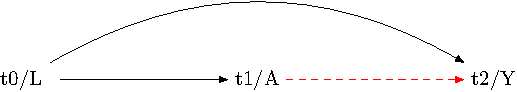
\includegraphics[width=0.8\textwidth,height=\textheight]{causal-dags_files/figure-pdf/fig-dag-common-cause-1.pdf}

}

\caption{\label{fig-dag-common-cause}Counfounding by a common cause. The
dashed path indicates bias arising from the open backdoor path from A to
Y.}

\end{figure}

\hypertarget{advice-attend-to-the-temporal-order-of-all-measured-variables}{%
\subsubsection{Advice: attend to the temporal order of all measured
variables}\label{advice-attend-to-the-temporal-order-of-all-measured-variables}}

Addressing confounding by a common cause involves its adjustment. This
adjustment effectively closes the backdoor path from the exposure to the
outcome. Equivalently, conditioning on \(L\) d-separates \(A\) and
\(Y\). Common adjustment methods include regression, matching, inverse
probability of treatment weighting, and G-methods (covered in
(\protect\hyperlink{ref-hernuxe1n2023a}{Hernán and Robins 2023b})).
Figure~\ref{fig-dag-common-cause-solution} clarifies that any confounder
that is a common cause of both \(A\) and \(Y\) must precede \(A\) (and
hence \(Y\)), since effects follow their causes chronologically.

By time-indexing the nodes on the graph, we immediately understand that
\textbf{control of confounding generally necessitates time-series data.}
Our causal diagram is a circuit breaker that casts doubt on attempts for
causal inference in settings where researchers lack time series data.

\begin{figure}

{\centering 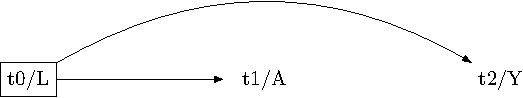
\includegraphics[width=0.8\textwidth,height=\textheight]{causal-dags_files/figure-pdf/fig-dag-common-cause-solution-1.pdf}

}

\caption{\label{fig-dag-common-cause-solution}Solution: adjust for
pre-exposure confounder.}

\end{figure}

\hypertarget{confounding-by-collider-stratification-conditioning-on-a-common-effect}{%
\subsubsection{2. Confounding by collider stratification (conditioning
on a common
effect)}\label{confounding-by-collider-stratification-conditioning-on-a-common-effect}}

Conditioning on a common effect occurs when a variable \(L\) is affected
by the treatment \(A\) and an outcome \(Y\).

Suppose \(A\) and \(Y\) are initially independent, such that
\(A \coprod Y(a)\). Conditioning on the joint effect \(L\) opens a
backdoor path between \(A\) and \(Y\), potentially inducing a non-causal
association. This occurs because \(L\) can provide information about
both \(A\) and \(Y\).

To clarify, let \(A\) denote the level of belief in Big Gods (with
higher values indicating stronger belief), \(Y\) denote social
complexity, and \(L\) denote economic trade. Suppose that belief in Big
Gods and social complexity were not causally linked. That is, if we were
to intervene to foster such beliefs, this intervention would not itself
affect social complexity. However, suppose beliefs in Big Gods and
social complexity separately influence levels of economic trade (\(L\)).
Now suppose we were to condition on economic trade without attending to
temporal order -- perhaps because time series data are not available. In
that case, we might find a statistical association between belief in Big
Gods and social complexity without a causal association.\footnote{To
  clarify, denote the observed associations as follows:

  \begin{itemize}
  \tightlist
  \item
    \(P(A)\): Distribution of beliefs in Big Gods
  \item
    \(P(Y)\): Distribution of social complexity
  \item
    \(P(L)\): Distribution of economic trade
  \end{itemize}

  Without conditioning on \(L\), if \(A\) and \(Y\) are independent, we
  have:

  \[P(A, Y) = P(A)P(Y)\]

  However, if we condition on \(L\) (which is a common effect of both
  \(A\) and \(Y\)), we have:

  \[P(A, Y | L) \neq P(A | L)P(Y | L)\]

  Once conditioned on, the common effect \(L\) creates an association
  between \(A\) and \(Y\) that is not causal. This association in the
  data can mislead us into believing there is a direct link between
  beliefs in Big Gods and social complexity, even without such a link.
  If we were to only observed \(A\), \(Y\), and \(L\) in cross-sectional
  data, we might erroneously conclude \(A \to Y\)

  When \(A\) and \(Y\) are independent, the joint probability of \(A\)
  and \(Y\) is equal to the product of their individual probabilities:
  \(P(A, Y) = P(A)P(Y)\). However, when we condition on \(L\), the joint
  probability of \(A\) and \(Y\) given \(L\) is not necessarily equal to
  the product of the individual probabilities of \(A\) and \(Y\) given
  \(L\), hence the inequality \(P(A, Y | L) \neq P(A | L)P(Y | L)\).}

\begin{figure}

{\centering 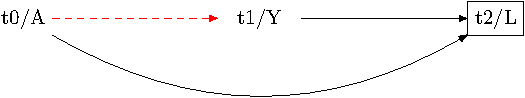
\includegraphics[width=0.8\textwidth,height=\textheight]{causal-dags_files/figure-pdf/fig-dag-common-effect-1.pdf}

}

\caption{\label{fig-dag-common-effect}Confounding by conditioning on a
collider. The dashed red path indicates bias from the open backdoor path
from A to Y.}

\end{figure}

\hypertarget{advice-attend-to-the-temporal-order-of-all-measured-variables-1}{%
\subsubsection{Advice: attend to the temporal order of all measured
variables}\label{advice-attend-to-the-temporal-order-of-all-measured-variables-1}}

To address the problem of conditioning on a common effect, we should
\emph{generally} ensure that:

\begin{enumerate}
\def\labelenumi{\arabic{enumi}.}
\tightlist
\item
  all confounders \(L\) that are common causes of the exposure \(A\) and
  the outcome \(Y\) are measured before \(A\) has occurred, and
\item
  \(A\) is measured before \(Y\) has occurred.
\end{enumerate}

If such temporal order is preserved, \(L\) cannot be an effect of \(A\),
and thus neither of \(Y\).\footnote{This rule is not absolute. As
  indicated in Figure~\ref{fig-dag-descendent-solution}, it may be
  helpful in certain circumstances to condition on a confounder that
  occurs after the outcome has occurred.} In the example just described
for beliefs and social complexity, such assurance typically requires
time-series data with accurate measurements. Also required is a
sufficiently large sample of cultures that transition in religious
beliefs, with measurements of social complexity before and after.
Moreover, the cultures in the dataset would need to be independent of
each other.\footnote{The independence of cultural units was at the
  centre of the study of comparative urban archaeology from the late
  19th (\protect\hyperlink{ref-decoulanges1903}{De Coulanges 1903})
  through the late 20th century
  (\protect\hyperlink{ref-wheatley1971}{Wheatley 1971}). Despite
  attention to this problem in recent work (e.g.
  (\protect\hyperlink{ref-watts2016}{Watts \emph{et al.} 2016})), there
  is arguably a greater head-room for understanding the need for
  conditional independence of cultures in recent cultural evolutionary
  studies. Again, attending to the temporal order of events is
  essential.}

\begin{figure}

{\centering 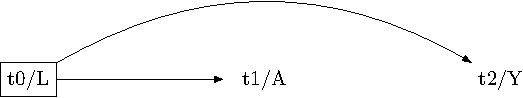
\includegraphics[width=0.8\textwidth,height=\textheight]{causal-dags_files/figure-pdf/fig-dag-common-effect-solution-1.pdf}

}

\caption{\label{fig-dag-common-effect-solution}Solution: time idexing of
confounders helps to avoid collider bias and maintain d-separation. The
graph makes the imperative clear: we must collect time series data with
confounders measured before the exposure, and that we must likewise
measure the exposure before the outcome, with data collected
repeatitively on the same units.}

\end{figure}

\hypertarget{m-bias-conditioning-on-a-collider-that-occurs-before-the-exposure-may-introduce-bias}{%
\subsubsection{M-bias: conditioning on a collider that occurs before the
exposure may introduce
bias}\label{m-bias-conditioning-on-a-collider-that-occurs-before-the-exposure-may-introduce-bias}}

Typically, indicators for confounders should be included only if they
are known to be measured before their exposures - with notable
exceptions described below in fig-dag-descendent-solution-2 and .

However, researchers should also be cautious about over-conditioning on
pre-exposure variables that are not associated with both the exposure
and confounder, as doing so can induce confounding. As shown in
Figure~\ref{fig-m-bias}, collider stratification may arise even if \(L\)
occurs before \(A\). This happens when \(L\) does not affect \(A\) or
\(Y\), but may be the descendent of an unmeasured variable that affects
\(A\) and another unmeasured variable that also affects \(Y\).
Conditioning on \(L\) in this scenario evokes ``M-bias.'' If \(L\) is
not a common cause of \(A\) and \(Y\), or the effect of a shared common
cause, \(L\) should not be included in a causal model.
Figure~\ref{fig-m-bias} presents a case in which \(A \coprod Y(a)\) but
\(A \cancel{\coprod} Y(a)| L\). M-bias is another example of collider
stratification bias (see: (\protect\hyperlink{ref-cole2010}{Cole
\emph{et al.} 2010})).\footnote{Note, when we draw a chronologically
  ordered path from left to right the M shape for which ``M-bias'' takes
  its name changes to an E shape We shall avoid every temptation to
  proliferate jargon and call it M bias.}

\begin{figure}

{\centering 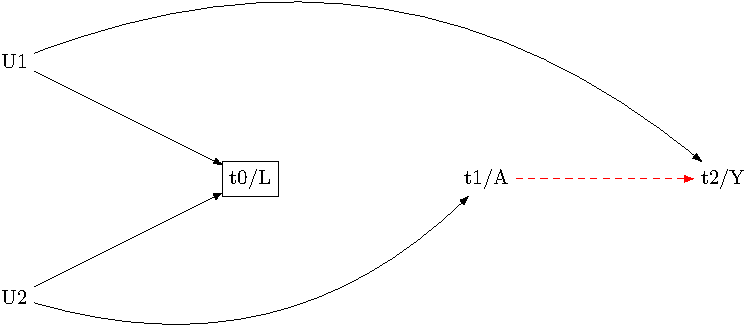
\includegraphics[width=0.8\textwidth,height=\textheight]{causal-dags_files/figure-pdf/fig-m-bias-1.pdf}

}

\caption{\label{fig-m-bias}M-bias: confounding control by including
previous outcome measures. The dashed red path indicates bias from the
open backdoor path from A to Y by conditioning on pre-exposure variable
L. The solution: do not condition on L. The graph makes it evident that
conditioning on variables measured before the exposure is not sufficient
to prevent confounding.}

\end{figure}

\hypertarget{advice-adopt-the-modified-disjunctive-cause-criterion-for-confounding-control}{%
\subsubsection{Advice: adopt the modified disjunctive cause criterion
for confounding
control}\label{advice-adopt-the-modified-disjunctive-cause-criterion-for-confounding-control}}

Again, the modified disjunctive cause criterion will satisfy the
backdoor criterion in all cases and reduce bias where this criterion
cannot be fully satisfied:

\begin{enumerate}
\def\labelenumi{\alph{enumi}.}
\tightlist
\item
  Control for any variable that causes the exposure, the outcome, or
  both.
\item
  Control for any proxy for an unmeasured variable that is a shared
  cause of both exposure and outcome.
\item
  Define an instrumental variable as a variable associated with the
  exposure but does not influence the outcome independently, except
  through the exposure. Exclude any instrumental variable that is not a
  proxy for an unmeasured confounder from the confounder set (see:
  VanderWeele \emph{et al.}
  (\protect\hyperlink{ref-vanderweele2020}{2020}) page 441,
  (\protect\hyperlink{ref-vanderweele2019}{VanderWeele 2019}))
\end{enumerate}

Of course, the difficulty is in determining which variables belong to a
confounder set. Specialist knowledge can facilitate this task. However,
the data alone typically do not settle this question. (For exceptions
see: bulbulia2021).

\hypertarget{mediator-bias}{%
\subsubsection{3. Mediator bias}\label{mediator-bias}}

Conditioning on a mediator -- a variable that lies along the causal
pathway between the treatment and the outcome -- can distort the total
effect of the treatment on the outcome and potentially introduce bias.
To illustrate this, consider ``beliefs in Big Gods'' as the treatment
(\(A\)), ``social complexity'' as the outcome (\(Y\)), and ``economic
trade'' as the mediator (\(L\)).

In this scenario, the belief in Big Gods (\(A\)) has a direct impact on
economic trade (\(L\)), which subsequently influences social complexity
(\(Y\)). If we condition on economic trade (\(L\)), we could bias our
estimates of the overall effect of beliefs in Big Gods (\(A\)) on social
complexity (\(Y\)). This bias happens because conditioning on \(L\) can
downplay the direct effect of \(A\) on \(Y\), as it blocks the indirect
path through \(L\). This problem, known as mediator bias, is illustrated
in Figure~\ref{fig-dag-mediator}.

We might think that conditioning on a mediator does not introduce bias
under a null hypothesis (\(A\) does not cause \(Y\)), however, this is
not the case. Consider a situation where \(L\) is a common effect of the
exposure \(A\) and an unmeasured variable \(U\) linked to the outcome
\(Y\). In this scenario, including \(L\) may amplify the association
between \(A\) and \(Y\), even if \(A\) is not associated with \(Y\) and
\(U\) does not cause \(A\). This scenario is represented in
Figure~\ref{fig-dag-descendent}.

So, unless one is explicitly investigating mediation analysis, it is
usually not advisable to condition on a post-treatment variable. Again,
attending to chronology in the the spatial organisation of the graph
reveals an imperative for data collection: if we cannot ensure that
\(L\) is measured before \(A\), and if \(A\) may affect \(L\), including
\(L\) in our model could result in mediator bias. This scenario is
presented in Figure~\ref{fig-dag-descendent}.

\begin{figure}

{\centering 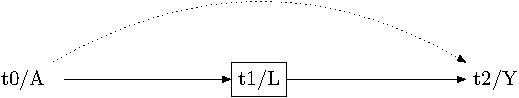
\includegraphics[width=0.8\textwidth,height=\textheight]{causal-dags_files/figure-pdf/fig-dag-mediator-1.pdf}

}

\caption{\label{fig-dag-mediator}Confounding by conditioning on a
mediator. The dashed black arrow indicates bias arising from partially
blocking the path between A and Y.}

\end{figure}

\hypertarget{advice-attend-to-the-temporal-order-of-all-measured-variables-2}{%
\subsubsection{Advice: attend to the temporal order of all measured
variables}\label{advice-attend-to-the-temporal-order-of-all-measured-variables-2}}

To mitigate the issue of mediator bias, particularly when focusing on
total effects, we should generally avoid conditioning on a mediator. We
avoid this problem by ensuring that \(L\) occurs before the treatment
\(A\) and the outcome \(Y\) (Note: a counter-example is presented in
Figure~\ref{fig-dag-descendent-solution-2}). Again, we discover the
importance of explicitly stating the temporal ordering of our
variables.\footnote{Note that if \(L\) were associated with \(Y\) and
  could not be caused by \(A\), conditioning on \(L\) would typically
  enhance the precision of the causal effect estimate of \(A \to Y\).
  This precision enhancement holds even if \(L\) occurs after \(A\).
  However, the onus is on the researcher to show that the post-treatment
  factor cannot be a consequence of the exposure.}

\begin{figure}

{\centering 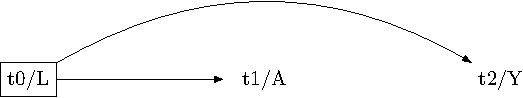
\includegraphics[width=0.8\textwidth,height=\textheight]{causal-dags_files/figure-pdf/fig-dag-mediator-solution-1.pdf}

}

\caption{\label{fig-dag-mediator-solution}By indexing nodes we discover
the problem. It is generally imperative that confounders are measured
prior to the exposure. Blue path indicates L no longer d-separates A and
Y, allowing for unbiased effect estimate.}

\end{figure}

\hypertarget{conditioning-on-a-descendant-man-induce-confounding}{%
\subsubsection{4. Conditioning on a descendant man induce
confounding}\label{conditioning-on-a-descendant-man-induce-confounding}}

Say \(L\) is a cause of \(L^\prime\). According to Markov factorisation,
if we condition on \(L\), we partially condition on \(L^\prime\).

Consider how conditioning might imperil causal estimation. Suppose there
is a confounder \(L^\prime\) that is caused by an unobserved variable
\(U\), and is affected by the treatment \(A\). Suppose further that
\(U\) causes the outcome \(Y\). In this scenario, as described in
Figure~\ref{fig-dag-descendent}, conditioning on \(L^\prime\), which is
a descendant of \(A\) and \(U\), can lead to a spurious association
between \(A\) and \(Y\) through the path \(A \to L^\prime \to U \to Y\).

\begin{figure}

{\centering 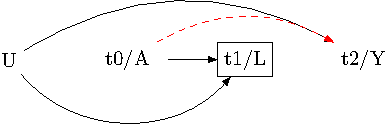
\includegraphics[width=0.8\textwidth,height=\textheight]{causal-dags_files/figure-pdf/fig-dag-descendent-1.pdf}

}

\caption{\label{fig-dag-descendent}Confounding by descent: the red
dashed path illustrates the introduction of bias from the opening of a
backdoor path between the exposure, A, and the outcome, Y, when
conditioning on a descendant of a confounder. Red path indicates bias}

\end{figure}

Again, the advice is evident from the chronology of the graph: we should
measure the (\(L^\prime\)) before the exposure (\(A\)). This solution is
presented in Figure~\ref{fig-dag-descendent-solution}.

\begin{figure}

{\centering 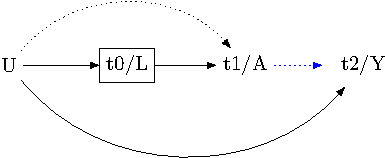
\includegraphics[width=0.8\textwidth,height=\textheight]{causal-dags_files/figure-pdf/fig-dag-descendent-solution-1.pdf}

}

\caption{\label{fig-dag-descendent-solution}Solution: again, ensure
temporal ordering for all measured variables. By ensuring that L occurs
before A confounding is controlled. Graph aslo makes evident that L need
not affect Y to be a confounder (i.e.~a member of either an ajustment or
confounder set.)}

\end{figure}

\hypertarget{conditioning-on-a-descendent-may-reduce-confounding}{%
\subsubsection{5. Conditioning on a descendent may reduce
confounding}\label{conditioning-on-a-descendent-may-reduce-confounding}}

Next consider how we may use a post-treatment descendent to reduce bias.
Suppose an unmeasured confounder \(U\) affects \(A\), \(Y\), and
\(L^\prime\) as presented in, then adjusting for \(L^\prime\) may help
to reduce confounding caused by \(U\). This scenario is presented in
Figure~\ref{fig-dag-descendent-solution-2}. If we deploy the modified
disjunctive cause criterion for confounding control, we would ``include
as a covariate any proxy for an unmeasured variable that is a common
cause of both the exposure and the outcome''
(\protect\hyperlink{ref-vanderweele2019}{VanderWeele 2019}). We discover
that although \(L^\prime\) may occur \emph{after} the exposure, and
indeed occur \emph{after} the outcome, we may condition on it to reduce
confounding because it is a proxy for an unmeasured common cause of the
exposure and the confounder. \textbf{This example shows that employing a
rule that requires us to condition only on pre-exposure (and indeed
pre-outcome) variables would be hasty.} More generally,
fig-dag-descendent-solution-2 demonstrates the imperative for thinking
carefully about data collection. We cannot blindly apply alogrithic
rules about confounding control. Each problem must be approached anew.

\begin{figure}

{\centering 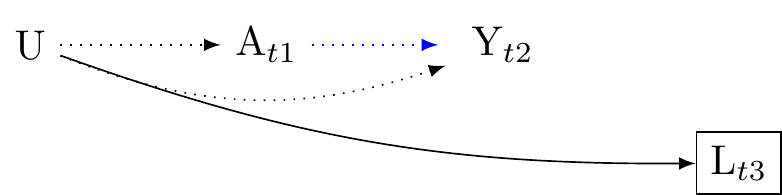
\includegraphics[width=0.8\textwidth,height=\textheight]{causal-dags_files/figure-pdf/fig-dag-descendent-solution-2-1.pdf}

}

\caption{\label{fig-dag-descendent-solution-2}Solution: conditioning on
a confounder that occurs after the exposure and the outcome may address
a problem of unmeasured confounding if the confounder is a descendent of
a prior common cause of the exposure and outcome. The dotted paths
denote that the effect of U on A and Y is partially adjusted by
conditioning on L', even though L' occurs after the outcome. The dotted
paths represent biased reduced by conditioning on the post-outcome
descendent of an unmeasured common cause of the exposure and outcome.
For example, a genetic factor that affects the exposure and the outcome
early in life might be measured by an indicator late that is expressed
(and may be measured) later in life. Adjusting for such an indicator
would constitute an example of post-outcome confounding control.}

\end{figure}

\hypertarget{case-1-causal-interaction-and-causal-effect-modification-do-not-draw-non-linear-relationships-such-as-interactions}{%
\subsubsection{Case 1: Causal Interaction and Causal Effect
Modification: do not draw non-linear relationships such as
interactions}\label{case-1-causal-interaction-and-causal-effect-modification-do-not-draw-non-linear-relationships-such-as-interactions}}

Interactions are scientific interesting because we often wish to
understand for whom effects occur. How shall we depict interactions on a
graph? It is crucial to remember the primary function of causal diagrams
is to investigate confounding. Causal diagrams are not designed to
capture all facets of a phenomenon under investigation. We should not
attempt any unique visual trick to show additive and multiplicative
interaction. Moreover, we should include those nodes and paths as are
necessary to evaluate structural sources of bias. Causal graphs are
meant to be human read. They are not meant to be complete maps of causal
reality.

Misunderstandings arise about the role and function of causal diagrams
in application to interaction. Such misunderstandings typically stem
from a more profound confusion about the concept of interaction itself.
Given this deeper problem, it is worth clarifying the concept of causal
interaction as understood within the counterfactual causal framework.
Again, evaluating evidence for interaction is often essential for much
scientific research. However, we must distinguish between concepts of
causal interaction and concepts of causal effect modification because
these concepts address different causal questions.

\hypertarget{causal-interaction-as-a-double-exposure}{%
\paragraph{\texorpdfstring{\textbf{Causal interaction as a double
exposure}}{Causal interaction as a double exposure}}\label{causal-interaction-as-a-double-exposure}}

Causal interaction refers to the combined or separate (or non-existent)
effect of two exposures. Evidence for interaction on a given scale is
present when the effect of one exposure on an outcome depends on another
exposure's level. For instance, the impact of beliefs in Big Gods
(exposure A) on social complexity (outcome Y) might depend on a
culture's monumental architecture (exposure B), which could also
influence social complexity. Evidence of causal interaction on the
difference scale would be present if:

\[\bigg(\underbrace{\mathbb{E}[Y(1,1)]}_{\text{joint exposure}} - \underbrace{\mathbb{E}[Y(0,0)]}_{\text{neither exposed}}\bigg) - \bigg[ \bigg(\underbrace{\mathbb{E}[Y(1,0)]}_{\text{only A exposed}} - \underbrace{\mathbb{E}[Y(0,0)]}_{\text{neither exposed}}\bigg) + \bigg(\underbrace{\mathbb{E}[Y(0,1)]}_{\text{only B exposed}} - \underbrace{\mathbb{E}[Y(0,0)]}_{\text{neither exposed}} \bigg)\bigg] \neq 0 \]

This equation simplifies to

\[ \underbrace{\mathbb{E}[Y(1,1)]}_{\text{joint exposure}} - \underbrace{\mathbb{E}[Y(1,0)]}_{\text{only A exposed}} - \underbrace{\mathbb{E}[Y(0,1)]}_{\text{only B exposed}} + \underbrace{\mathbb{E}[Y(0,0)]}_{\text{neither exposed}} \neq 0 \]

If the above equation were to hold, the effect of exposure \(A\) on the
outcome \(Y\) would differ across levels of \(B\) or vice versa. Such a
difference would provide evidence for interaction.

If the value is positive, we say there is evidence for an additive
effect. If the value is less than zero, we say there is evidence for a
sub-additive effect. If the value is virtually zero, there is no
reliable evidence for interaction.\footnote{Note that causal effects of
  interactions often differ when measured on the ratio scale. This
  discrepency can have significant policy implications, see:
  (\protect\hyperlink{ref-vanderweele2014}{VanderWeele and Knol 2014}).
  Although beyond the scope of this article, when evaluating evidence
  for causality we must clarify the measure of effect in which we are
  interested (\protect\hyperlink{ref-hernuxe1n2004}{Hernán \emph{et al.}
  2004}; \protect\hyperlink{ref-tripepi2007}{Tripepi \emph{et al.}
  2007}).}

Remember that causal diagrams are non-parametric. They do not directly
represent interactions. They are tools for addressing the identification
problem. Although a causal diagram can indicate an interaction's
presence by displaying two exposures jointly influencing an outcome, as
in Figure~\ref{fig-dag-interaction}, it does not directly represent the
interaction's nature or scale.

\begin{figure}

{\centering 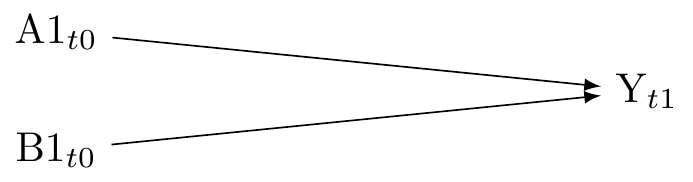
\includegraphics[width=0.6\textwidth,height=\textheight]{causal-dags_files/figure-pdf/fig-dag-interaction-1.pdf}

}

\caption{\label{fig-dag-interaction}Causal interaction: if two exposures
are causally independent of each other, we may wish to estimate their
individual and joint effects on Y, where the counterfactual outcome is
Y(a,b) and there is evidence for additive or subadditive interaction if
E{[}Y(1,1) - Y(0,1) - Y(1,0) + Y(0,0){]} ≠ 0. If we cannot conceptualise
B as a variable upon which intervention can occur, then the interaction
is better conceived as effect modification (see next figure). Important:
do not attempt to draw a path into another path.}

\end{figure}

\hypertarget{causal-effect-modification-under-a-single-exposure}{%
\paragraph{\texorpdfstring{\textbf{Causal effect modification under a
single
exposure}}{Causal effect modification under a single exposure}}\label{causal-effect-modification-under-a-single-exposure}}

With the analysis of effect modification, we aim to understand how an
exposure's effect varies, if at all, across levels of another variable,
an effect modifier.

Consider again the problem of estimating the causal effect of beliefs in
Big Gods on social complexity. Suppose this time we are interested in
the investigating whether this effect varies across early urban
civilisations in ancient China and South America. In this example
geography (China versus South America) is an ``effect modifier.'' Here,
we do not treat the effect modifier as an intervention. Rather, we wish
to investigate whether geography is a parameter that may alter the
exposure's effect on an outcome.

For clarity, consider comparing two exposure levels, represented as
\(A = a\) and \(A= a^*\). Further, assume that \(G\) represents two
levels of effect-modification, represented as \(g\) and \(g'\).

Then, the expected outcome when exposure is at level \(A=a\) among
individuals in group \(G=g\) is expressed

\[\hat{E}[Y(a)|G=g]\]

The expected outcome when exposure is at level \(A=a^*\) among
individuals in group \(G=g\) is expressed

\[\hat{E}[Y(a^*)|G=g]\]

The causal effect of shifting the exposure level from \(a^*\) to \(a\)
in group \(g\) is expressed

\[\hat{\delta}_g = \hat{\mathbb{E}}[Y(a)|G=g] - \hat{\mathbb{E}}[Y(a^*)|G=g]\]

Likewise, the causal effect of changing the exposure from \(a^*\) to
\(a\) in group \(g'\) is expressed.

\[\hat{\delta}_{g'} = \hat{\mathbb{E}}[Y(a)|G=g'] - \hat{\mathbb{E}}[Y(a^*)|G=g']\]

We compare the causal effect on the difference scale in these two groups
by computing

\[\hat{\gamma} = \hat{\delta}_g - \hat{\delta}_{g'}\]

The value of \(\hat{\gamma}\) quantifies how the effect of shifting the
exposure from \(a^*\) to \(a\) differs between groups \(g\) and \(g'\).

If \(\hat{\gamma}\neq 0\), then there is evidence for effect
modification. We may infer the exposure's effect varies by geography.

Again, remember that causal diagrams are non-parametric. More
fundamental, causal diagrams function to identify structural sources of
bias and to help researchers develop strategies for addressing such
bias. We should not draw an intersecting path or attempt other
visualisations to represent effect modification. Instead, we should draw
two edges into the exposure. This is depicted in
Figure~\ref{fig-dag-effect-modfication}.\footnote{For distinctions
  within varieties of effect modification relevant for strategies of
  confounding controul see
  (\protect\hyperlink{ref-vanderweele2007}{VanderWeele and Robins
  2007b}).}

\begin{figure}

{\centering 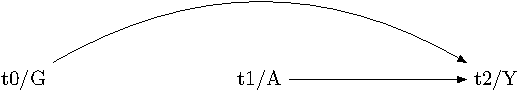
\includegraphics[width=0.8\textwidth,height=\textheight]{causal-dags_files/figure-pdf/fig-dag-effect-modfication-1.pdf}

}

\caption{\label{fig-dag-effect-modfication}A simple graph for
effect-modification in which there are no confounders. G is an effect
modifier of A on Y. We draw a box around G to indicate we are
conditioning on this variable.}

\end{figure}

\hypertarget{case-2-causal-mediation-causal-diagrams-reveal-the-inadequacy-of-standard-approaches}{%
\subsubsection{Case 2: Causal Mediation: causal diagrams reveal the
inadequacy of standard
approaches}\label{case-2-causal-mediation-causal-diagrams-reveal-the-inadequacy-of-standard-approaches}}

The conditions necessary for causal mediation are stringent. I present
these conditions in the chronologically ordered causal diagram shown in
Figure~\ref{fig-dag-mediation-assumptions}. We will again consider
whether cultural beliefs in Big Gods affect social complexity. Let us
also ask whether this affect is mediated by political authority. The
assumptions required for asking causal mediation questions are as
follows

\begin{enumerate}
\def\labelenumi{\arabic{enumi}.}
\tightlist
\item
  \textbf{No unmeasured exposure-outcome confounders given} \(L\)
\end{enumerate}

This prerequisite is expressed as \(Y(a,m) \coprod A | L1\). Upon
controlling for the covariate set \(L1\), we must ensure that no
additional unmeasured confounders affect both the cultural beliefs in
Big Gods \(A\) and the social complexity \(Y\). For example, suppose our
study involves the effect of cultural beliefs in Big Gods (exposure) on
social complexity (outcome), and geographic location and historical
context define the covariates in \(L1\). In that case, we must assume
that accounting for \(L1\) d-separates \(A\) and \(Y\). The relevant
confounding path is depicted in brown in
Figure~\ref{fig-dag-mediation-assumptions}.

\begin{enumerate}
\def\labelenumi{\arabic{enumi}.}
\setcounter{enumi}{1}
\tightlist
\item
  \textbf{No unmeasured mediator-outcome confounders given} \(L\)
\end{enumerate}

This condition is expressed as \(Y(a,m) \coprod M | L2\). After
controlling for the covariate set \(L2\), we must ensure that no other
unmeasured confounders affect the political authority \(M\) and social
complexity \(Y\). For instance, if trade networks impact political
authority and social complexity, we must account for trade networks to
obstruct the unblocked path linking our mediator and outcome. Further,
we must assume the absence of any other confounders for the
mediator-outcome path. This confounding path is represented in blue in
Figure~\ref{fig-dag-mediation-assumptions}.

\begin{enumerate}
\def\labelenumi{\arabic{enumi}.}
\setcounter{enumi}{2}
\tightlist
\item
  \textbf{No unmeasured exposure-mediator confounders given} \(L\)
\end{enumerate}

This requirement is expressed as \(M(a) \coprod A | L3\). Upon
controlling for the covariate set \(L3\), we must ensure that no
additional unmeasured confounders affect both the cultural beliefs in
Big Gods \(A\) and political authority \(M\). For example, the
capability to construct large ritual theatres may influence the belief
in Big Gods and the level of political authority. If we have indicators
for this technology measured prior to the emergence of Big Gods (these
indicators being \(L3\)), we must assume that accounting for \(L3\)
closes the backdoor path between the exposure and the mediator. This
confounding path is shown in green in
Figure~\ref{fig-dag-mediation-assumptions}.

\begin{enumerate}
\def\labelenumi{\arabic{enumi}.}
\setcounter{enumi}{3}
\tightlist
\item
  \textbf{No mediator-outcome confounder affected by the exposure (no
  red arrow)}
\end{enumerate}

This requirement is expressed as \(Y(a,m) \coprod M(a^*) | L\). We must
ensure that no variables confounding the relationship between political
authority and social complexity in \(L2\) are themselves influenced by
the cultural beliefs in Big Gods (\(A\)). For instance, when studying
the effect of cultural beliefs in Big Gods (\(A\), the exposure) on
social complexity (\(Y\), the outcome) as mediated by political
authority (mediator), there can be no factors, such as trade networks
(\(L2\)), that influence both political authority and social complexity
and are affected by the belief in Big Gods. This confounding path is
shown in red in Figure~\ref{fig-dag-mediation-assumptions}. \textbf{Note
that the assumption of no exposure-induced confounding in the
mediator-outcome relationship is often a substantial obstacle for causal
mediation analysis.} If the exposure influences a confounder of the
mediator and outcome, we face a dilemma. Without accounting for this
confounder, the backdoor path between the mediator and the outcome
remains open. By accounting for it, however, we partially obstruct the
path between the exposure and the mediator, leading to bias.
Consequently, observed data cannot identify the natural direct and
indirect effects.

Notice again that the requirements for counterfactual data science are
more strict than for descriptive or predictive data science.

We have now considered how chronologically ordered causal diagrams
elucidate the conditions necessary for causal mediation
analysis.\footnote{An excellent resource both for understanding causal
  interaction and causal mediation is
  (\protect\hyperlink{ref-vanderweele2015}{VanderWeele 2015}).}

\begin{figure}

{\centering \includegraphics[width=0.8\textwidth,height=\textheight]{causal-dags_files/figure-pdf/fig-dag-mediation-assumptions-1.pdf}

}

\caption{\label{fig-dag-mediation-assumptions}Assumptions for mediation
analysis. The brown edges denote the path for common causes of the
exposure and coutcome. To block this path we must condition on L1. The
green edges denote the path for common causes of the exposure and
mediator. To block this path we must condition on L3. The blue edges
denote the path for common causes of the mediator and outcome. To block
this path we must condition on L2. The red path denotes the effect of
the exposure on the confounder of the mediator and outcome. If any such
path exists then we cannot obtain natural direct and indirect effects.
Conditioning on L2 is necessary to prevent mediator-outcome confounding
but doing so blocks the effect of the exposure on the mediator. The
dashed paths indicates potential for bias in natural direct and indirect
causal effect estimates if all four assumptiions for causal mediation
are not satisfied.}

\end{figure}

\hypertarget{case-3-confounder-treatment-feedback-longitudinal-growth-is-not-causation}{%
\subsubsection{Case 3: Confounder-Treatment Feedback: Longitudinal
``growth'' is not
causation}\label{case-3-confounder-treatment-feedback-longitudinal-growth-is-not-causation}}

In our discussion of causal mediation, we consider how the effects of
two sequential exposures may combine to affect an outcome. We can
broaden this interest to consider the causal effects of multiple
sequential exposures. In such scenarios, causal diagrams arranged
chronologically can aid in clarifying the challenges and opportunities.

For example, consider temporally fixed multiple exposures. The
counterfactual outcomes may be denoted \(Y(a_{t1} ,a_{t2})\). There are
four counterfactual outcomes corresponding to the four fixed ``treatment
regimes'':

\begin{enumerate}
\def\labelenumi{\arabic{enumi}.}
\item
  \textbf{Always treat (Y(1,1))}
\item
  \textbf{Never treat (Y(0,0))}
\item
  \textbf{Treat once first (Y(1,0))}
\item
  \textbf{Treat once second (Y(0,1))}
\end{enumerate}

\hypertarget{tbl-regimes}{}
\begin{longtable}[]{@{}
  >{\raggedright\arraybackslash}p{(\columnwidth - 4\tabcolsep) * \real{0.1351}}
  >{\raggedright\arraybackslash}p{(\columnwidth - 4\tabcolsep) * \real{0.5405}}
  >{\raggedright\arraybackslash}p{(\columnwidth - 4\tabcolsep) * \real{0.3243}}@{}}
\caption{\label{tbl-regimes}Table describes four fixed treatment regimes
and six causal contrasts in time series data where the exposure may
vary.}\tabularnewline
\toprule\noalign{}
\begin{minipage}[b]{\linewidth}\raggedright
Type
\end{minipage} & \begin{minipage}[b]{\linewidth}\raggedright
Description
\end{minipage} & \begin{minipage}[b]{\linewidth}\raggedright
Counterfactual Outcome
\end{minipage} \\
\midrule\noalign{}
\endfirsthead
\toprule\noalign{}
\begin{minipage}[b]{\linewidth}\raggedright
Type
\end{minipage} & \begin{minipage}[b]{\linewidth}\raggedright
Description
\end{minipage} & \begin{minipage}[b]{\linewidth}\raggedright
Counterfactual Outcome
\end{minipage} \\
\midrule\noalign{}
\endhead
\bottomrule\noalign{}
\endlastfoot
Regime & Always treat & Y(1,1) \\
Regime & Never treat & Y(0,0) \\
Regime & Treat once first & Y(1,0) \\
Regime & Treat once second & Y(0,1) \\
Contrast & Always treat vs.~Never treat & E{[}Y(1,1) - Y(0,0){]} \\
Contrast & Always treat vs.~Treat once first & E{[}Y(1,1) - Y(1,0){]} \\
Contrast & Always treat vs.~Treat once second & E{[}Y(1,1) -
Y(0,1){]} \\
Contrast & Never treat vs.~Treat once first & E{[}Y(0,0) - Y(1,0){]} \\
Contrast & Never treat vs.~Treat once second & E{[}Y(0,0) - Y(0,1){]} \\
Contrast & Treat once first vs.~Treat once second & E{[}Y(1,0) -
Y(0,1){]} \\
\end{longtable}

There are six causal contrasts that we might compute for the four fixed
regimes, presented in Table~\ref{tbl-regimes}.\footnote{We compute the
  number of possible combinations of contrasts by
  \(C(n, r) = \frac{n!}{(n-r)! \cdot r!}\)}

Not that treatment assignments might be sensibly approached as a
function of the previous outcome. For example, we might \textbf{treat
once first} and then decide whether to treat again depending on the
outcome of the initial treatment. This aspect is known as ``time-varying
treatment regimes.''

Bear in mind that to estimate the ``effect'' of a time-varying treatment
regime, we are obligated to make comparisons between the relevant
counterfactual quantities. As mediation can introduce the possibility of
time-varying confounding (condition 4: the exposure must not impact the
confounders of the mediator/outcome path), the same holds true for all
sequential time-varying treatments. However, unlike conventional causal
mediation analysis, it might be necessary to consider the sequence of
treatment regimes over an indefinitely long period.

Chronologically organised causal diagrams are useful for highlighting
problems with traditional multi-level regression analysis and structural
equation modelling.

For example, we might be interested in whether belief in Big Gods
affects social complexity. Consider estimating a fixed treatment regime
first. Suppose we have a well-defined concept of Big Gods and social
complexity as well as excellent measurements for both over time. In that
case, we might want to assess the effects of beliefs in Big Gods on
social complexity, say, two centuries after the beliefs were introduced.

The fixed treatment strategies are: ``always believe in Big Gods''
versus ``never believe in Big Gods'' on the level of social complexity.
Refer to Figure~\ref{fig-dag-9}. Here, \(A_{tx}\) represents the
cultural belief in Big Gods at time \(tx\), and \(Y_{tx}\) is the
outcome, social complexity, at time \(x\). Imagine that economic trade,
denoted as \(L_{tx}\), is a time-varying confounder. Suppose its effect
changes over time, which in turns affects the factors that influence
economic trade. To complete our causal diagram, we might include an
unmeasured confounder \(U\), such as oral traditions, which could
influence both the belief in Big Gods and social complexity.

Consider a scenario where we can reasonably infer that the level of
economic trade at time \(0\), represented as \(L_{t0}\), impacts beliefs
in ``Big Gods'' at time \(1\), denoted as \(A_{t1}\). In this case, we
would draw an arrow from \(L_{t0}\) to \(A_{t1}\). Conversely, if we
assume that belief in ``Big Gods'', \(A_{t1}\), influences the future
level of economic trade, \(L_{t2}\), then an arrow should be added from
\(A_{t1}\) to \(L_{t2}\). This causal diagram illustrates a feedback
process between the time-varying exposure \(A\) and the time-varying
confounder \(L\). Figure ``dag-9'' displays exposure-confounder
feedback. In practical settings, the diagram could contain more arrows.
However, the intention here is to use the minimal number of arrows
needed to demonstrate the issue of exposure-confounder feedback. As a
guideline, we should avoid overcomplicating our causal diagrams and aim
to include only the essential details necessary for assessing the
identification problem.

What would happen if we were to condition on the time-varying confounder
\(L_{t3}\)? Two things would occur. First, we would block all the
backdoor paths between the exposure \(A_{t2}\) and the outcome. We need
to block those paths to eliminate confounding. Therefore, conditioning
on the time-varying confounding is essential. However, paths that were
previously blocked would close. For example, the path
\(A_{t1}, L_{t2}, U, Y_{t4}\), that was previously closed would be
opened because the time-varying confounder is the common effect of
\(A_{t1}\) and \(U\). Conditioning, then, opens the path
\(A_{t1}, L_{t2}, U, Y_{t4}\). Therefore we must avoid conditioning on
the time-varying confounder. It would seem then that if we were to
condition on a confounder that is affected by the prior exposure, we are
``damned if we do'' and ``dammed if we do not.''

\begin{figure}

{\centering 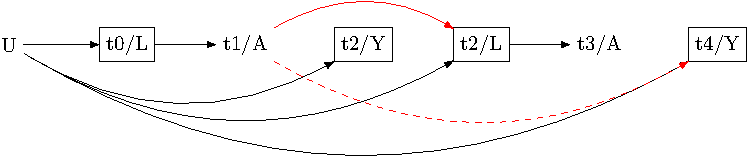
\includegraphics[width=1\textwidth,height=\textheight]{causal-dags_files/figure-pdf/fig-dag-9-1.pdf}

}

\caption{\label{fig-dag-9}Exposure confounder feedback is a problem for
time-series models. If we do not condition on L\_t2, a backdoor path is
open from A\_t3 to Y\_t4. However, if conditioning on L\_t2 introduces
collider bias, opening a path, coloured in red, between A\_t2 and Y\_t4.
Here, we may not use conventional methods to estimate the effects of
multiple exposures. Instead, at best, we may obtain controlled effects
using G-methods. Multi-level models will not eliminate bias (!).
However, outside of epidemiology, G-methods are presently too rarely
used.}

\end{figure}

A similar problem arises when a time-varying exposure and time-varying
confounder share a common cause. This problem arises even without the
exposure affecting the confounder. The problem is presented in
Figure~\ref{fig-dag-time-vary-common-cause-A1-l1}.

\begin{figure}

{\centering 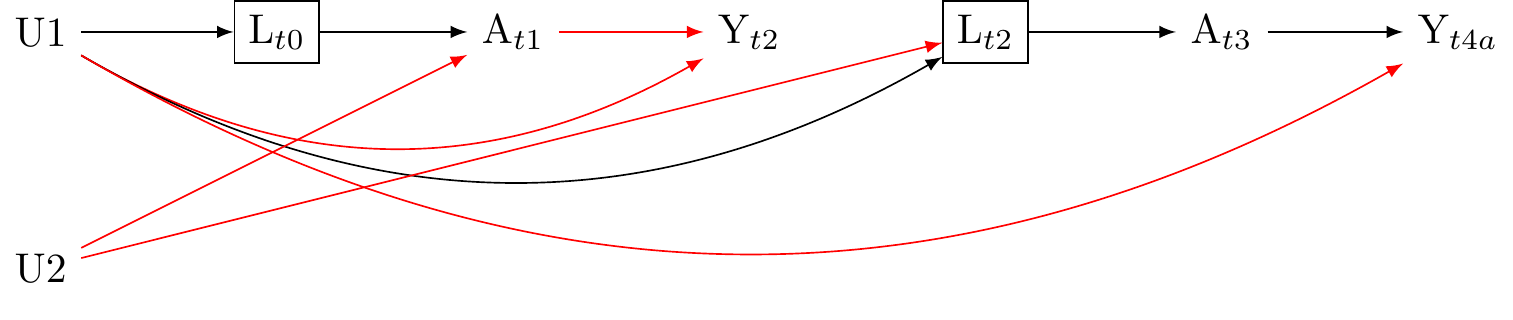
\includegraphics[width=1\textwidth,height=\textheight]{causal-dags_files/figure-pdf/fig-dag-time-vary-common-cause-A1-l1-1.pdf}

}

\caption{\label{fig-dag-time-vary-common-cause-A1-l1}Exposure confounder
feedback is a problem for time-series models. Here, the problem arises
from an unmeasured variable (U\_2) that affects both the exposure A at
time 1 and the cofounder L at time 2. The red paths show the open
backdoor path when we condition on the L at time 2. Again, we cannot
infer causal effects in such scenarios by using regression-based
methods. In this setting, to address causal questions, we require
G-methods.}

\end{figure}

The potential for confounding increases when the exposure \(A_{t1}\)
affects the outcome \(Y_{t4}\). For example, since \(L_{t2}\) is on the
path from \(A_{t1}\) to \(Y_{t4}\), conditioning on \(L_{t2}\) partially
blocks the relation between the exposure and the outcome, triggering
collider stratification bias and mediator bias. However, to close the
open backdoor path from \(L_{t2}\) to \(Y_{t4}\), it becomes necessary
to condition on \(L_{t2}\). Paradoxically, we have just stated that
conditioning should be avoided! This broader dilemma of
exposure-confounder feedback is thoroughly explored in
(\protect\hyperlink{ref-hernuxe1n2023}{Hernán and Robins 2023a}).
Treatment confounder feedback is particularly challenging for
evolutionary human science, yet its handling is beyond the capabilities
of conventional regression-based methods, including multi-level models
(\protect\hyperlink{ref-hernuxe1n2006}{Hernán and Robins 2006};
\protect\hyperlink{ref-robins1986}{Robins 1986};
\protect\hyperlink{ref-robins1999}{Robins \emph{et al.} 1999}). As
mentioned previously, ``G-methods'' encompass models appropriate for
investigating the causal effects of both time-fixed and time-varying
exposures (\protect\hyperlink{ref-chatton2020}{Chatton \emph{et al.}
2020}; \protect\hyperlink{ref-hernuxe1n2006}{Hernán and Robins 2006};
\protect\hyperlink{ref-naimi2017}{Naimi \emph{et al.} 2017}). Despite
significant recent advancements in the health sciences
(\protect\hyperlink{ref-breskin2020}{Breskin \emph{et al.} 2020};
\protect\hyperlink{ref-duxedaz2021}{Díaz \emph{et al.} 2021};
\protect\hyperlink{ref-williams2021}{Williams and Díaz 2021}), these
methods have not been widely embraced in the field of human evolutionary
sciences \footnote{It is worth noting that the identification of
  controlled effect estimates can be enhanced by graphical methods such
  as ``Single World Intervention Graphs'' (SWIGs), which represent
  counterfactual outcomes in the diagrams. However, SWIGs are more
  accurately considered templates rather than causal diagrams in their
  general form. The use of SWIGs extends beyond the scope of this
  tutorial. For more information, see Richardson and Robins
  (\protect\hyperlink{ref-richardson2013}{2013}).}

\hypertarget{summary-part-2}{%
\subsubsection{Summary Part 2}\label{summary-part-2}}

To consistently estimate causal effects, we must contrast the world as
it has been with the world as it might have been. For many questions in
evolutionary human science, we have seen that confounder-treatment
feedback leads to intractable causal identification problems. We have
also seen that causal diagrams are helpful in clarifying these problems.
Many self-inflicted injuries, such as mediator bias and
post-stratification bias, could be avoided if confounders were measured
prior to the exposures. Chronologically ordered causal diagrams aim to
make this basis transparent. They are the circuit-breakers that helpt to
prevent us from blowing up our causal inferences. More constructively,
the focus attention on imperatives for data collection, which if
followed, offer hope.

\hypertarget{part-3.-an-application-of-chronologically-ordered-causal-diagrams-to-confounding-bias-for-data-collection-the-three-wave-panel-design}{%
\subsection{Part 3. An Application of Chronologically Ordered Causal
Diagrams to Confounding Bias for Data Collection: The Three-Wave Panel
Design}\label{part-3.-an-application-of-chronologically-ordered-causal-diagrams-to-confounding-bias-for-data-collection-the-three-wave-panel-design}}

In the following discussion, the focus is on the application of
temporally ordered causal diagrams as tools to guide researchers in
planning efficient data collection. Note that I use the term ``wave''
without defining a specific period. Causes must precede effects, but the
amount of time needed to assess causality will vary depending on the
phenomena of interest. Note that in a causal diagram, \textbf{intervals
need not be drawn to scale}, however when specifying research, the
appropriate interval of measurement will depend on the interests and
purposes of a study. To minimise the propect of unmeasured time-varying
confounders to arise between the baseline condition and the exposure
events, it is generally useful to reduce the the length of this baseline
to exposure interval where doing so is possible. If the object of
interest is a rare event (such as religious conversion) such short
measurement interval separating baseline from exposure might not be
feasible.

\hypertarget{step-1.-defining-the-exposure-measure-it-at-wave-0-and-wave-1}{%
\subsubsection{Step 1. Defining the exposure: measure it at wave 0 and
wave
1}\label{step-1.-defining-the-exposure-measure-it-at-wave-0-and-wave-1}}

We begin with a well-defined exposure. Unless our study objectives
revolve around causal interactions, causal mediation, or sequential
treatment plans, our primary goal would typically be to investigate the
total effect of a singular exposure.

Consider the causal effect of attending religious services. The first
critical step involves defining the exposure in the context of a
hypothetical intervention. What aspect is of interest to us? Is it a
comparison of attendance versus non-attendance? Are we distinguishing
between weekly and monthly attendees? Perhaps, we are interested in a
different facet altogether? Visualising a hypothetical experiment - even
when it is not feasible - reveals the need for a precise intervention
specification (\protect\hyperlink{ref-bulbulia2022}{Bulbulia 2022};
\protect\hyperlink{ref-hernuxe1n2016a}{Hernán \emph{et al.} 2016b};
\protect\hyperlink{ref-hernuxe1n2022}{Hernán \emph{et al.} 2022b}).

The exposure is measured at wave 1 (i.e.~+1 interval from baseline, wave
0). When estimating causal effects, the inclusion of exposure at the
baseline carries three critical advantages:

\begin{enumerate}
\def\labelenumi{\alph{enumi}.}
\tightlist
\item
  \textbf{Incidence effect interpretation}: incorporating the baseline
  exposure allows us to interpret the effect of exposure measured
  post-baseline as an incidence effect, not a prevalence effect
  (\protect\hyperlink{ref-vanderweele2020}{VanderWeele \emph{et al.}
  2020}). This means we can interpret the effect as the change due to a
  new occurrence (incidence) of the exposure, rather than the overall
  presence (prevalence) of the exposure. For example, in a study
  investigating the impact of weekly religious service attendance,
  including the baseline measure of attendance enables us to understand
  the effect of starting to attend weekly services (incidence), as
  opposed to simply being a regular attendee (prevalence).
\end{enumerate}

\begin{enumerate}
\def\labelenumi{\arabic{enumi}.}
\setcounter{enumi}{1}
\item
  \textbf{Confounding control}: the baseline exposure's inclusion helps
  to reduce unmeasured confounding arising from time-invariant
  confounders. These are variables that do not change over time and
  could confound the association between the exposure and the outcome if
  not properly accounted for. For instance, personal attributes such as
  unmeasured childhood religiosity could confound the association
  between religious service attendance and outcomes if not considered
  (\protect\hyperlink{ref-vantongeren2020}{Van Tongeren \emph{et al.}
  2020}).
\item
  \textbf{Better evaluation of sample adequacy for rare exposures}:
  Particularly when the exposure is uncommon, such as switching from no
  religious service attendance to weekly attendance, measuring the
  baseline exposure and outcome exposure can help assess adequacy of a
  sample size. Suppose this switch occurs rarely in the non-religious
  population, say 1 in 1,000 non-attenders per year. To estimate causal
  effects while conditioning on a rich set of baseline covariates, we
  would need a large sample, potentially comprising hundreds of
  thousands of participants. Ideally researchers would understake
  investigations prior to data collection to assess feasiblity of causal
  inference. In this example, it might be more practical to examine
  changes within the religious population, that is -- assuming changes
  are more common within this group -- than it would be to investigate
  conversion events. However, by restricting to only religious people
  who change in their religious habits, we would then typically estimate
  a causal effect generalisable to the religious population from which
  the sample was drawn, rather than one that could be applied to the
  non-religious population. In any case, including the baseline exposure
  can help address these issues by providing a reference point for
  changes within the population studied.
\end{enumerate}

\hypertarget{step-2.-specify-the-outcomes-measure-them-at-wave-0-and-wave-2}{%
\subsubsection{Step 2. Specify the Outcome(s): Measure them at wave 0
and wave
2}\label{step-2.-specify-the-outcomes-measure-them-at-wave-0-and-wave-2}}

After defining the exposure, we need to determine a well-defined outcome
(or potentially several outcomes). For instance, we might be interested
in understanding the effect of acquiring or losing religious service
attendance on the frequency of volunteering (e.g., weekly, monthly,
yearly). We have seen that statements like ``the causal effects of
religious change'' are not insightful. We must articulate clearly the
phenomenon under study and its timing (e.g., the +1-year effect on
weekly volunteering from a shift of 0 to weekly or more religious
service attendance).

Measuring the outcome at baseline offers several advantages:

\begin{enumerate}
\def\labelenumi{\alph{enumi}.}
\item
  \textbf{Temporal ordering}: controlling for the baseline measure of
  the outcome helps confirm the temporal order of the cause-effect
  relationship, thereby guarding against reverse causation.
\item
  \textbf{Confounding control}: when we also control for the exposure at
  baseline, an unmeasured confounder would have to negate the
  association between the exposure at one wave post-baseline and the
  outcome at two waves post-baseline, independent of the baseline
  effect, as show in Figure~\ref{fig-dag-6}. Note, this figure shows
  that \textbf{reduction of bias is preferable to no reduction if bias}.
  This is an important practical point: although it may not be possible
  to eliminate all confounding (the dashed arrows symbolise potential
  sources of uncontrolled bias), the processes of data collection and
  analysis can help reduce it. Putting this point more sharply, there is
  a great danger in allowing automated confounding control strategies to
  govern an analysis. Again, a minimal adjustment set cannot be insured.
  Our task is always to reduce confounding in the presence of unmeasured
  confounders. A strategy must be carefully considered at the design
  phase in light both of the problem at hand, and the data that might be
  collected.\footnote{Given the typical uncertainty about having
    accounted for all unmeasured confounding, it is prudent for
    researchers to conduct sensitivity analyses
    (\protect\hyperlink{ref-shi2021}{Shi \emph{et al.} 2021}).}
\end{enumerate}

\begin{enumerate}
\def\labelenumi{\alph{enumi}.}
\setcounter{enumi}{2}
\tightlist
\item
  \textbf{Robustness checks}: baseline measures provide a foundation for
  conducting additional robustness checks and sensitivity analyses. They
  may allow for the detection of outliers or errors in data collection
  and help researchers understand the stability of the measured
  phenomena over time.
\end{enumerate}

\begin{figure}

{\centering 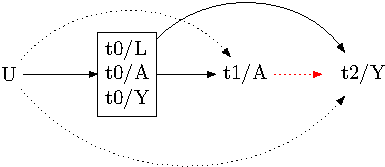
\includegraphics[width=0.8\textwidth,height=\textheight]{causal-dags_files/figure-pdf/fig-dag-6-1.pdf}

}

\caption{\label{fig-dag-6}Causal diagram adapted from Vanderweele et
al.'s three-wave panel design. The dotted line indicates a reduction in
bias arising from including baseline measures for the exposure and
outcome. For an unmeasured confounder U to bias the exposure-outcome
association, it would need to do so independently of these outcome and
exposure baseline measures. The graph clarifies that by measuring
confounders before the exposure and the exposure before the outcome, we
reduce the potential for reverse causation, collider stratification, and
mediator biases.}

\end{figure}

\hypertarget{step-3.-identify-observable-common-causes-of-the-exposure-and-the-outcome}{%
\subsubsection{Step 3. Identify observable common causes of the exposure
and the
outcome}\label{step-3.-identify-observable-common-causes-of-the-exposure-and-the-outcome}}

Next, we should identify all the potential confounders that, when
adjusted for, can eliminate any non-causal association between the
exposure and outcome. We should group these confounders under standard
labels wherever they share the same functional dependencies in the
graph. In a three-wave panel design, confounders are recorded during the
baseline wave. As illustrated in Figure~\ref{fig-dag-mediator-solution},
recording confounders before the occurrence of the exposure minimises
the potential for mediation bias. For example in Figure~\ref{fig-dag-6},
the variable \(L\) on the graph might denote rich set of indicators such
as Age, Gender, Education,Political Orientation, SES,\(\dots\) Again,
causal diagrams are meant to be human read. We should not include these
additional nodes when including a single node will suffice for clarity
and thoroughness.

\hypertarget{step-4.-gather-data-for-proxy-variables-of-unmeasured-common-causes-at-the-baseline-wave}{%
\subsubsection{Step 4. Gather data for proxy variables of unmeasured
common causes at the baseline
wave}\label{step-4.-gather-data-for-proxy-variables-of-unmeasured-common-causes-at-the-baseline-wave}}

Recall Figure~\ref{fig-dag-descendent-solution-2}: if any unmeasured
confounders influence both the exposure and outcome, but we lack direct
measurements, we should make efforts to include proxies for them. Again,
even if this strategy cannot eliminate all bias from unmeasured
confounding, it will generally reduce bias.

\hypertarget{step-5.-state-the-target-population-for-whom-the-causal-question-applies}{%
\subsubsection{Step 5. State the target population for whom the causal
question
applies}\label{step-5.-state-the-target-population-for-whom-the-causal-question-applies}}

We need to define for whom our causal inference applies. For this
purpose, it is helpful to distinguish the concepts of source population
and target population and between the concepts of generalisability and
transportability.

\begin{enumerate}
\def\labelenumi{\arabic{enumi}.}
\item
  \textbf{The source population} is the population from whom our sample
  is drawn.
\item
  \textbf{The target population} is the larger population for whom we
  aim to apply our study's results. The closer the source population
  matches the target population in structural features relevant to our
  causal questions, the stronger our causal inferences about the target
  population will be.
\item
  \textbf{Generalisability}: when the causal effect estimated from a
  sample applies to the target population beyond the sample population,
  we say the causal effect estimates are generalisable. This concept is
  also known as ``external validity.''
\end{enumerate}

Let \(PATE\) denote the population average treatment effect for the
target population. Let \(ATE_{\text{source}}\) denote the average
treatment effect in the source population. Let \(W\) denote a set of
variables upon which the source and target population structurally
differ. We say that results \emph{generalise} if there is a function
such that

\[PATE =  f(ATE_{\text{source}}, W)\]

\begin{enumerate}
\def\labelenumi{\arabic{enumi}.}
\setcounter{enumi}{3}
\tightlist
\item
  \textbf{Transportability}: when causal effects estimates may
  generalise to different settings and populations from which the source
  population was sampled, we say effects are transportable. Where \(T\)
  denotes a set of variables upon which the source and the target
  population structurally differ, we say that results are transportable
  if there is a function such that
\end{enumerate}

\[ATE_{\text{target}} \approx f(ATE_{\text{source}}, T)\]

This function similarly maps the average treatment effect from the
source population to a target population. The function over \(T\) might
be more complex, as it must handle potential heterogeneity of effects
and unobserved sources of bias. To assess transportability, we generally
require information about the source and target populations and a
specialist understanding. In Section 4, we will return to the concepts
of generalisability and transportability as they pertain to sample
selection.

\hypertarget{step-6.-retention-is-a-top-priority}{%
\subsubsection{Step 6. Retention is a top
priority}\label{step-6.-retention-is-a-top-priority}}

Sample retention is a mission-critical imperative for reasons we clarify
in Part 4. Panel attrition opens novel pathways for bias. Researchers
must develop protocols for tracking individuals as they change
addresses, emails, phone numbers, and names. Moreover, developing and
implementing strategies for motivating retention across the entire
population of interest (not merely those willing to volunteer for
science) is critical for causal human science. These strategies must be
developed with specialist knowledge of the population under study and
the participation and insights of the people being studied.

\hypertarget{summary-of-part-3}{%
\subsubsection{Summary of Part 3}\label{summary-of-part-3}}

The strengths of three-wave panel designs for confounding control are
demonstrated in Figure~\ref{fig-dag-6}. This diagram, adapted from
VanderWeele \emph{et al.}
(\protect\hyperlink{ref-vanderweele2020}{2020}), highlights the
potential for residual unmeasured confounding even after incorporating
baseline measurements for both the exposure and outcome, represented by
the blue-dotted line. As such, for an unmeasured confounder \(U\) to
exert bias on the association between the exposure \(A_{t1}\) and
outcome \(Y_{t2}\), it must do so independently of the baseline
measurements of the exposure \(A_{t0}\) and outcome \(Y_{t0}\).

The diagram also reveals the advantage of three-wave panel designs for
addressing reverse causation. This control is achieved by adjusting for
both the exposure and outcome at baseline, ensuring the temporal
sequence causality required. Moreover, the diagram underscores the
capacity of three-wave panel designs to yield estimates for the
incidence, not just the prevalence, of effects.

A further understanding gained from Figure~\ref{fig-dag-6} is related to
the potential risks associated with collider stratification and mediator
bias. As discussed in Part 2, bias may arise from conditioning on a
variable measured after treatment. We can significantly reduce such
biases by ensuring the measurement of confounders takes place before the
exposure and by ensuring that the exposure is measured before the
outcome.

Figure~\ref{fig-dag-6} emphasises the crucial role of understanding both
confounding and confoundign control before collecting repeated measures
data. Nonetheless, VanderWeele \emph{et al.}
(\protect\hyperlink{ref-vanderweele2020}{2020})'s causal diagram does
not account for potential selection bias from panel attrition. In Part
4, we will develop this causal diagram to clarify such challenges.

\hypertarget{part-4.-applications-of-chronologically-ordered-causal-diagrams-for-understanding-selection-bias}{%
\subsection{Part 4. Applications of Chronologically Ordered Causal
Diagrams for Understanding Selection
Bias}\label{part-4.-applications-of-chronologically-ordered-causal-diagrams-for-understanding-selection-bias}}

\hypertarget{introduction-to-selection-bias}{%
\subsubsection{Introduction to selection
bias}\label{introduction-to-selection-bias}}

Selection bias arises when the parameter of interest in the target
population and the equivalent parameter in a subset of this population
used for analysis, the source population, do not align
(\protect\hyperlink{ref-hernuxe1n2017}{Hernán 2017}). To understand
selection bias, consider the following topology of confounding developed
by Suzuki and colleagues (\protect\hyperlink{ref-suzuki2016}{Suzuki
\emph{et al.} 2016}; \protect\hyperlink{ref-suzuki2020}{Suzuki \emph{et
al.} 2020}; \protect\hyperlink{ref-suzuki2014}{Suzuki and Yamamoto
2014}).\footnote{This typology builds on VanderWeele's work
  (\protect\hyperlink{ref-vanderweele2012}{VanderWeele and Hernán
  2012}).}

\begin{enumerate}
\def\labelenumi{\arabic{enumi}.}
\item
  \textbf{Confounding in distribution}: if the sample exposed to each
  level of exposure is representative of the target population, we say
  there is no confounding in the distribution of the exposure's effect
  on the outcome.
\item
  \textbf{Confounding in expectation}: if the exposure assignment
  mechanism balances the confounders across each level of contrast in
  the exposure, we say there is no confounding in the expectation of the
  exposure's effect on the outcome.
\item
  \textbf{Confounding in measure}: if a specific measure of interest
  matches the corresponding causal measure in the target population, we
  say there is no confounding in the measure of the exposure's effect on
  the outcome. As discussed previously concerning interaction, our
  inference of a causal effect can depend on the scale of the causal
  effect measure.
\item
  \textbf{Realised confounding}: if a specific exposure assignment leads
  to balance, irrespective of the exposure assignment mechanism, we say
  there is no realised confounding of the exposure's effect on the
  outcome. This concept is essential because, even in randomised
  experiments, randomisation might not eliminate chance imbalances in
  the distributions of confounders across the exposures.
\end{enumerate}

Each of these four concepts plays a role in ``confounding'' discussions,
and all are crucial when evaluating a study's scientific merit. However,
each concept highlights different issues.

Armed with these distinctions, consider
Figure~\ref{fig-selection-under-the-null}, which presents a scenario
with no (marginal) causal effect of exposure on the outcome, yet a
degree of selection into the study. We will assume randomisation
succeeded so there are no arrows into \(A\). As
Figure~\ref{fig-selection-under-the-null} shows, neither confounding in
expectation nor confounding in distribution is present. Failure to
detect an association will accurately reflect the actual state of causal
disassociation in the population. We might say that selection leads to
``confounding in distribution for confounding in expectation.'' More
simply, we might say that despite selection, the null effect in the
source population is not biased for the target population
(\protect\hyperlink{ref-greenland1977}{Greenland 1977};
\protect\hyperlink{ref-hernuxe1n2004}{Hernán \emph{et al.}
2004}).\footnote{Note we use the term ``null effect'' as a structural
  concept. There are no statistical ``null effects.'' Instead there are
  reliable or unreliable statistical effect estimates according to some
  measure of evidence and arbitrary threshold
  (\protect\hyperlink{ref-bulbulia2021}{Bulbulia \emph{et al.} 2021}).}

\begin{figure}

{\centering 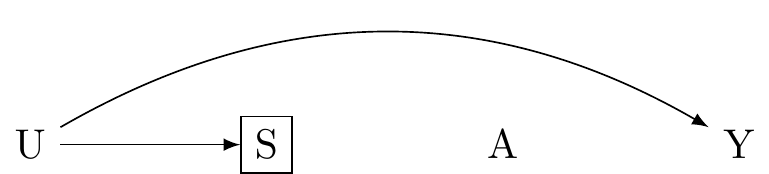
\includegraphics[width=0.6\textwidth,height=\textheight]{causal-dags_files/figure-pdf/fig-selection-under-the-null-1.pdf}

}

\caption{\label{fig-selection-under-the-null}Selection under the null.
An unmeasured variable affects the selection for the study and the
outcome. D-separation is preserved; there is no confounding in
expectation.}

\end{figure}

Figure~\ref{fig-selection-off-the-null} presents a different scenario in
which there is selection bias for the population parameter: the
association in the population of selected individuals differs from the
causal association for the target population. Hernán calls this scenario
``selection bias off the null''
(\protect\hyperlink{ref-hernuxe1n2017}{Hernán 2017}). Lu et al.~call
this scenario ``type 2 selection bias''
(\protect\hyperlink{ref-lu2022}{Lu \emph{et al.} 2022}). Such bias
occurs because the selection into the study occurs on an effect modifier
for the effect of the exposure on the outcome. Note that although the
causal effect of \(A\to Y\) is unbiased for the exposed and unexposed in
the source population, the effect estimate does not generalise to the
exposed and unexposed in the target population:
\(PATE \cancel{\approx} ATE_{\text{selected sample}}\).

\begin{figure}

{\centering 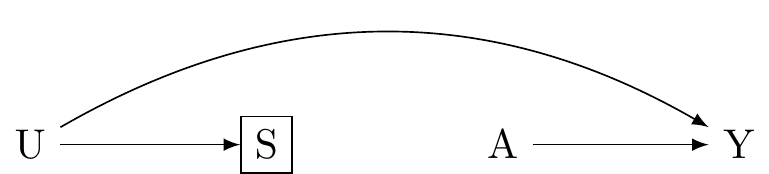
\includegraphics[width=0.6\textwidth,height=\textheight]{causal-dags_files/figure-pdf/fig-selection-off-the-null-1.pdf}

}

\caption{\label{fig-selection-off-the-null}Selection off the null: an
unmeasured variable affects selection into the study and the outcome.
Here the exposure affects the outcome. Selection, then, is an effect
modifier. Although d-separation is preserved, there is `confounding in
distribution'.}

\end{figure}

There has been considerable technical research investigating the
conditions under which causal estimates for a target population may be
identified when the source population differs from the target population
(see: (\protect\hyperlink{ref-lu2022}{Lu \emph{et al.} 2022})). There
has also been considerable technical research investigating the
conditions in which results might transport to populations that
systematically differ from the source population (see:
(\protect\hyperlink{ref-bareinboim2022}{Bareinboim \emph{et al.} 2022};
\protect\hyperlink{ref-deffner2022}{Deffner \emph{et al.} 2022};
\protect\hyperlink{ref-pearl2022}{Pearl and Bareinboim 2022})).To
address type 2 selection bias in a three-wave pane, we must accurately
measure and adjust for a sufficient set of covariates that affect
selection \(\framebox{S}\) (\protect\hyperlink{ref-lu2022}{Lu \emph{et
al.} 2022}). Moreover, when drawing causal diagrams, it is vital to
present confounding as it is assumed to exist in the target population,
not the source population (see Suzuki \emph{et al.}
(\protect\hyperlink{ref-suzuki2020}{2020}), especially their examples in
the supplement.) Practically speaking, where census data are available
these should be collected for constructing survey weights (see:
(\protect\hyperlink{ref-pishgar2021}{Pishgar \emph{et al.} 2021};
\protect\hyperlink{ref-stuart2015}{Stuart \emph{et al.} 2015})).

\hypertarget{selection-bias-in-which-both-the-exposure-and-outcome-affect-censoring}{%
\subsubsection{Selection bias in which both the exposure and outcome
affect
censoring}\label{selection-bias-in-which-both-the-exposure-and-outcome-affect-censoring}}

In panel designs, there is additionally a constant threat of selection
occurring \emph{after} enrolment into the study. We next put
chronological causal diagrams to use to make sense of this threat and
derive practical advice.

We next use causal diagrams to disclose biases arising from panel
attrition. Panel attrition can be viewed as a special case of selection
bias because the participants who continue in a longitudinal study may
differ from those who drop out in ways that generate structural biases.

Figure~\ref{fig-dag-8-5} describes a scenario in which both the exposure
and the true outcome affect panel attrition, biasing the observed
association between the exposure and the measured outcome in the
remaining sample. The problem of selection here is a problem of collider
stratification bias. We can equivalently view the problem as one of
directed measurement error, described in in
Figure~\ref{fig-dag-indep-d-effect}. Either way, restricting the
analysis to the retained sample introduces bias in the causal effect
estimate by opening a backdoor path from the exposure to the outcome. Lu
\emph{et al.} (\protect\hyperlink{ref-lu2022}{2022}) call this form of
bias: ``type 1 selection bias'' and distinguishes between scenarios when
causal effects that generalise are recoverable (type 1a selection bias)
and not recoverable (type 1b selection bias). In both cases, we must
develop strategies to evaluate whether we may recover from the subset of
the source population that has been censored, causal effect estimates
that generalise to a clearly defined target population.

\begin{figure}

{\centering 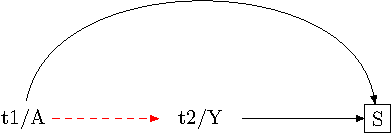
\includegraphics[width=0.8\textwidth,height=\textheight]{causal-dags_files/figure-pdf/fig-dag-8-5-1.pdf}

}

\caption{\label{fig-dag-8-5}Causal diagram in which outcome and exposure
affect attrition. Dashed red path shows correlation of A an Y in the
absence of causation.}

\end{figure}

\hypertarget{selection-bias-in-a-three-wave-panel}{%
\subsubsection{Selection bias in a three-wave
panel}\label{selection-bias-in-a-three-wave-panel}}

Figure~\ref{fig-dag-8} shows selection bias manifest in a three-wave
panel design when loss-to-follow-up results in a systematic disparity
between the baseline and follow-up source populations. The red dashed
lines in the diagram represent an open backdoor path, revealing a
potential indirect association between the exposure and the outcome.
Upon considering only the selected sample (i.e., when we condition on
the selected sample \(\framebox{S}\)), we may create or obscure
associations not evident in the source population at baseline.

\begin{figure}

{\centering 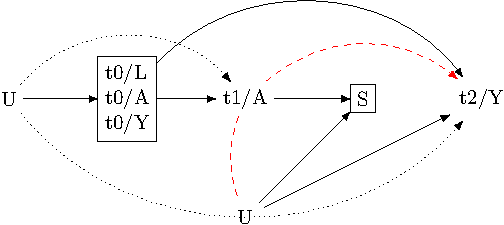
\includegraphics[width=0.8\textwidth,height=\textheight]{causal-dags_files/figure-pdf/fig-dag-8-1.pdf}

}

\caption{\label{fig-dag-8}Causal diagram of a three-wave panel design
with selection bias. Red paths reveal the open backdoor path induced by
conditioning on the selected sample.}

\end{figure}

\hypertarget{unmeasured-confounder-affects-outcome-and-variable-that-affects-attrition}{%
\subsubsection{Unmeasured confounder affects outcome and variable that
affects
attrition}\label{unmeasured-confounder-affects-outcome-and-variable-that-affects-attrition}}

Figure~\ref{fig-dag-8-2} presents another problem of selection bias in a
three-wave panel design. This diagram shows how an unmeasured
confounder, U\(_S\), can simultaneously influence the outcome variable
Y\(_{t2}\) and another variable, L\(_{t2}\), responsible for attrition
(i.e., the drop-out rate, denoted as \(\framebox{S}\)). Here we present
a scenario in which the exposure variable \(A_{t1}\) can impact a
post-treatment confounder L\(_{t2}\), which subsequently affects
attrition, \(\framebox{S}\). If the study's selected sample descends
from L\(_2\), the selection effectively conditions on L\(_{t2}\),
potentially introducing bias into the analysis. Figure~\ref{fig-dag-8-2}
marks this biasing pathway with red-dashed lines. Ordering the nodes
chronologically in the spatial design of one's graph clarifies the
assumed temporal sequence of events, allowing for a more precise
assessment of bias.

\begin{figure}

{\centering 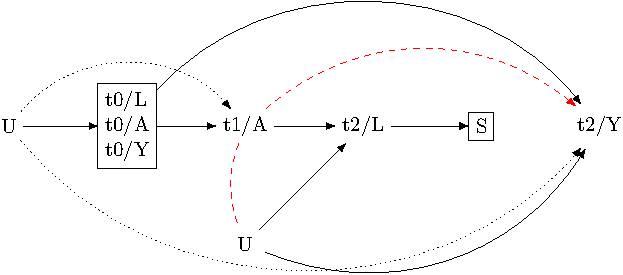
\includegraphics[width=0.8\textwidth,height=\textheight]{causal-dags_files/figure-pdf/fig-dag-8-2-1.pdf}

}

\caption{\label{fig-dag-8-2}Causal diagram of a three-wave panel design
with selection bias: Unmeasured confounder U\_S, is a cause of both of
the outcome Y\_2 and of a variable, L\_2 that affects attrition, S. The
exposure A affects this cause L\_2 of attrition, S. The selected sample
is a descendent of L\_2. Hence selection is a form of conditioning on
L\_2. Such conditioning opens a biasing path, indicated by the
red-dashed lines.}

\end{figure}

\hypertarget{why-regression-adjustment-fails-to-address-select-bias-from-attrition}{%
\subsubsection{Why regression adjustment fails to address select bias
from
attrition}\label{why-regression-adjustment-fails-to-address-select-bias-from-attrition}}

We cannot address selection bias from attrition using regression.
Shifting the example from culture to health, suppose that sicker
individuals or those with less successful outcomes are more likely to
drop out of the study. If this occurs, the remaining sample will not
represent the original population; it will over-represent healthier
individuals or those with more successful outcomes.

We use regression adjustment to control for confounding variables across
the treatment groups. With loss-to-follow-up, regression adjustment can
only address selection bias. The remaining censored population may
differ from the source population in the average association between the
exposure and the outcome.

What to do?

\begin{enumerate}
\def\labelenumi{\arabic{enumi}.}
\item
  \textbf{Retain sample}: the best way to deal with missing data is to
  prevent it in the first place. Maintain regular contact with study
  participants, using incentives for continued participation, making
  follow-ups as convenient as possible, and tracking participant details
  from multiple sources (email, phone, secondary contacts).
\item
  \textbf{Missing data imputation}: this requires predicting the missing
  values based on our data, assuming that the missingness is random
  conditional on baseline measures. Note that this missingness should be
  predicted separately within strata of the exposed and unexposed in the
  previous wave (see: (\protect\hyperlink{ref-westreich2015}{Westreich
  \emph{et al.} 2015}; \protect\hyperlink{ref-zhang2023}{Zhang \emph{et
  al.} 2023})). Imputation methods typically assume that data are
  missing conditional on a correctly specified model and information
  obtained at baseline.
\item
  \textbf{Inverse probability weighting with censoring weights}: this
  requires weighting the values of each participant in the study by the
  inverse of the probability of their observed pattern of missingness
  (censoring weights)(\protect\hyperlink{ref-cole2008}{Cole and Hernán
  2008}; \protect\hyperlink{ref-leyrat2019}{Leyrat \emph{et al.} 2019}).
  In this approach, the sample gives more weight to under-represented
  individuals owing to drop-out. As with missing data imputation, IPW
  with censoring weights also assumes that we can correctly model the
  missingness from the observed data
  (\protect\hyperlink{ref-shiba2021}{Shiba and Kawahara 2021}).
\item
  \textbf{Sensitivity analysis}: as with nearly all causal inference, we
  should quantitatively evaluate how sensitive results are to different
  assumptions and methods for handling censoring events
  (\protect\hyperlink{ref-shi2021}{Shi \emph{et al.} 2021}).
\end{enumerate}

\hypertarget{summary-of-part-4}{%
\subsubsection{Summary of Part 4}\label{summary-of-part-4}}

In this segment, we considered how causal diagrams may elucidate
confounding from selection bias. Selection bias can occur independently
of confounding bias. It manifests when the selection process for
participants in a study, or the dropout rates during the study, are
influenced by both the exposure and the outcome. The consequence is that
the observed exposure-outcome relationship in the study population
differs from the relationship that would have been observed in the
absence of such a selection process. Attending to selection bias is
essential at the design of research as well as its analysis. It suggest
the following strategies at design:

\begin{enumerate}
\def\labelenumi{\arabic{enumi}.}
\item
  \textbf{Broad sampling}: to ensure that the results of your study can
  be generalised, strive to sample extensively from the target
  population. A broad sample will offer more opportunities to measure
  all effect modifiers. With these data.
\item
  \textbf{Accurate measurement and adjustment for covariates}: in
  developing a three-wave panel, addressing type 2 selection bias
  requires precise measurements and appropriate confounding control
  (\protect\hyperlink{ref-lu2022}{Lu \emph{et al.} 2022}). Failing to
  measure and adjust for these covariates may lead to erroneous
  conclusions about the relationship between exposure and outcome.
\item
  \textbf{Construct causal diagrams for the target population}: causal
  diagrams should represent confounding as it exists in the target
  population (see Suzuki \emph{et al.}
  (\protect\hyperlink{ref-suzuki2020}{2020}), especially the
  supplementary materials provided).
\item
  \textbf{Maximise retention}: Rention is the mission-critical
  objective. In an nutshell the advise is: ``Rention, Retention,
  Retention!''
\end{enumerate}

Moreover, attention to selection bias suggests the following for
analysis:

\begin{enumerate}
\def\labelenumi{\arabic{enumi}.}
\setcounter{enumi}{4}
\item
  \textbf{Use multiple imputation or inverse probability of treatment
  with censoring weights to adjust for attrition} Achieving a 100\%
  retention rate is typically unattainable. To reduce disparities
  between the source population at baseline and the population from
  which the censored participants were drawn.
\item
  \textbf{Perform sensitivity analyses} to assess the robustness of
  results to methods for handling attrition.
\end{enumerate}

\hypertarget{part-5.-applications-of-chronologically-ordered-causal-diagrams-for-understanding-confounding-bias}{%
\subsection{Part 5. Applications of Chronologically Ordered Causal
Diagrams for Understanding Confounding
Bias}\label{part-5.-applications-of-chronologically-ordered-causal-diagrams-for-understanding-confounding-bias}}

In this section, we apply causal diagrams to illustrate the distinct
pathway of bias introduced by measurement error and discuss its
implications for research design. Unlike confounding bias, which arises
from the presence of a common cause of both the exposure and the
outcome, and selection bias, which arises from the participant selection
process or dropout rate, measurement bias arises from how variables are
measured or categorised.

\hypertarget{measurement-error-in-the-confounder}{%
\subsubsection{Measurement Error in the
Confounder}\label{measurement-error-in-the-confounder}}

Measurement error pervades all research. Figure
Figure~\ref{fig-dag-measure-confounder} demonstrates that even
error-free measurements of the exposure and outcome cannot counteract
the bias in causal effect estimates introduced by measurement error in
the confounders. Accurate measurement of confounders mitigates threats
to confounding. Once more, conducting a sensitivity analysis is
essential to evaluate the potential impact of this threat.\footnote{A
  simple yet powerful form of sensitivity analysis involves the
  computation of E-Values. E-Values calculate the minimal strength of
  association that an unmeasured confounder would require with both the
  exposure and outcome, beyond the measured confounders, to negate the
  observed exposure-outcome association (refer to the R package
  \texttt{EValue}:(\protect\hyperlink{ref-mathur2018}{Mathur \emph{et
  al.} 2018})).}

\begin{figure}

{\centering \includegraphics[width=0.6\textwidth,height=\textheight]{causal-dags_files/figure-pdf/fig-dag-measure-confounder-1.pdf}

}

\caption{\label{fig-dag-measure-confounder}Causal diagram showing a
confounder, L, measured with error, L'. Despite perfect measurements of
the exposure, A, and the outcome, Y, a bias-inducing (backdoor) path
opens between A - L - Y, highlighted in red. Given the ubiquity of
measurement error, it is imperative to minimise such errors and conduct
sensitivity analyses to assess the risk of unmeasured confounding.}

\end{figure}

Acknowledging the pervasiveness of measurement error and its potential
influence on our research, we will further explore how structural
approaches to understanding measurement error clarify the nature of the
problem, methods for adjustment, and the unceasing need for sensitivity
analyses.

Following Hernán and Cole (\protect\hyperlink{ref-hernuxe1n2009}{2009}),
we define structural concepts of measurement error and utilise causal
diagrams to understand how such errors may bias causal effect estimates.
A deeper understanding of these concepts (also explored by
(\protect\hyperlink{ref-vanderweele2012}{VanderWeele and Hernán 2012}),
will equip us to better manage and account for assessing bias from
measurement error in causal inference.

\hypertarget{uncorrelated-non-differential-undirected-measurement-error}{%
\subsubsection{1. Uncorrelated non-differential (undirected) measurement
error}\label{uncorrelated-non-differential-undirected-measurement-error}}

As shown in Figure~\ref{fig-dag-uu-null}, an uncorrelated
non-differential measurement error occurs when the errors in the
measurement of the exposure and outcome are not related.

To clarify, consider again the task of estimating the causal effect of
beliefs in Big Gods on social complexity. Suppose ancient societies
randomly omitted or recorded details about both beliefs in Big Gods and
indicators of social complexity in their records. Alternatively, suppose
that such records were not preserved equally across cultures for reasons
unrelated to these parameters. In this case, errors in the documentation
of both variables would be random. The errors would not be related to
the intensity of the beliefs in Big Gods or the level of social
complexity. The structure of this example of uncorrelated and
non-differential error is presented in Figure~\ref{fig-dag-uu-null}.

Uncorrelated non-differential measurement error does not create bias
under the null. As evident from Figure~\ref{fig-dag-uu-null},
d-separation is preserved. Equivalently, there are no open backdoor
paths on the graph. However, when there is an actual effect of the
exposure on the outcome, non-differential measurement error generally
leads to attenuated effect estimates. For this reason, uncorrelated
non-differential measurement error can be problematic for causal
inference even though they do not induce structural bias under the null.

\begin{figure}

{\centering 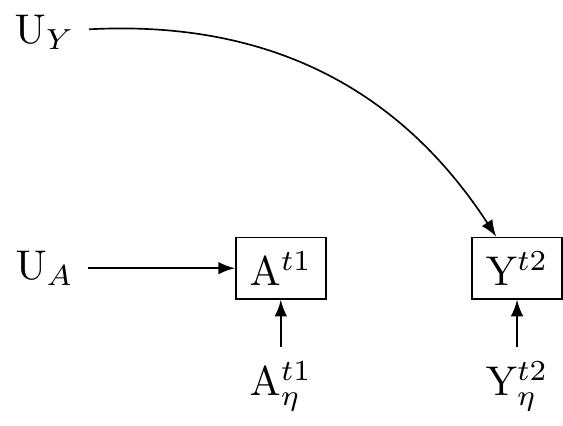
\includegraphics[width=0.6\textwidth,height=\textheight]{causal-dags_files/figure-pdf/fig-dag-uu-null-1.pdf}

}

\caption{\label{fig-dag-uu-null}Uncorrelated non-differential
measurement error does not bias estimates under the null, however may
attenuate true effects.}

\end{figure}

\hypertarget{uncorrelated-differential-directed-measurement-error}{%
\subsubsection{2. Uncorrelated differential (directed) measurement
error}\label{uncorrelated-differential-directed-measurement-error}}

As shown in Figure~\ref{fig-dag-indep-d-effect}, uncorrelated
differential (or directed) measurement error occurs when the measurement
errors are related to the level of exposure or outcome but not to each
other. For instance, societies with stronger beliefs in Big Gods might
have more or less detailed records of social complexity. Suppose that,
in the absence of any intervention on beliefs in Gods, there is no
association between the measurement errors. Here, the errors are
differential as they depend on the intensity of religious beliefs but
are uncorrelated as the errors in documenting beliefs in Big Gods and
social complexity are otherwise independent. Uncorrelated differential
(or directed) measurement error is presented in
Figure~\ref{fig-dag-indep-d-effect} and leads to bias under the null,
indicated by the red path. Equivalently, we may say that uncorrelated
differential (or directed) measurement error opens a backdoor path
between the exposure and the outcome.

Note that the bias presented in Figure~\ref{fig-dag-indep-d-effect}, an
example of directed measurement error, also describes the bias we
considered when there is panel attrition and which the exposure affects
selection (see: Figure~\ref{fig-dag-8-5}). In that scenario, the outcome
in the selected group is measured with error -- it no longer represents
the measurement of the outcome in the source population at baseline --
furthermore, this error is affected by exposure. The previous example
described bias in estimation from the vantage point of collider
stratification; however, we can also explain the distortion as directed
measurement bias.

\begin{figure}

{\centering 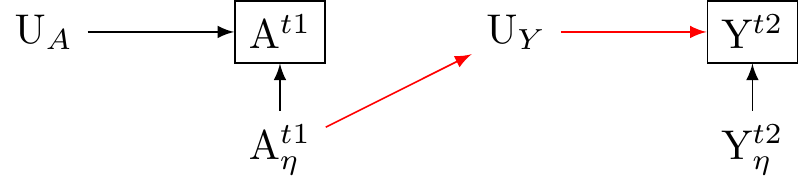
\includegraphics[width=1\textwidth,height=\textheight]{causal-dags_files/figure-pdf/fig-dag-indep-d-effect-1.pdf}

}

\caption{\label{fig-dag-indep-d-effect}Directed independent
(uncorrelated) measurement error can bias effect estimates under the
null. This bias is indicated by the red paths.}

\end{figure}

\hypertarget{correlated-non-differential-undirected-measurement-error}{%
\subsubsection{3. Correlated non-differential (undirected) measurement
error}\label{correlated-non-differential-undirected-measurement-error}}

As shown, Figure~\ref{fig-dag-dep-u-effect} correlated non-differential
(undirected) measurement error occurs when the errors in measuring both
the exposure and outcome are related independently of the exposure. The
scenario is presented in Figure~\ref{fig-dag-dep-u-effect}. Imagine that
some societies had more advanced record-keeping systems that resulted in
more accurate and detailed accounts of both beliefs in Big Gods and
social complexity. Furthermore, imagine that record keepers provide
better information about religious beliefs. In this case, the errors
between beliefs in Big Gods and social complexity are correlated because
the accuracy of records for both variables is influenced by the same
underlying factor (the record-keeping abilities). However, the errors
are not directed insofar as levels of religious beliefs and social
complexity do not affect the assumed bias in record keeping. Correlated
non-differential measurement error may induce bias under the null,
indicated by the red path in Figure~\ref{fig-dag-dep-u-effect}.

\begin{figure}

{\centering 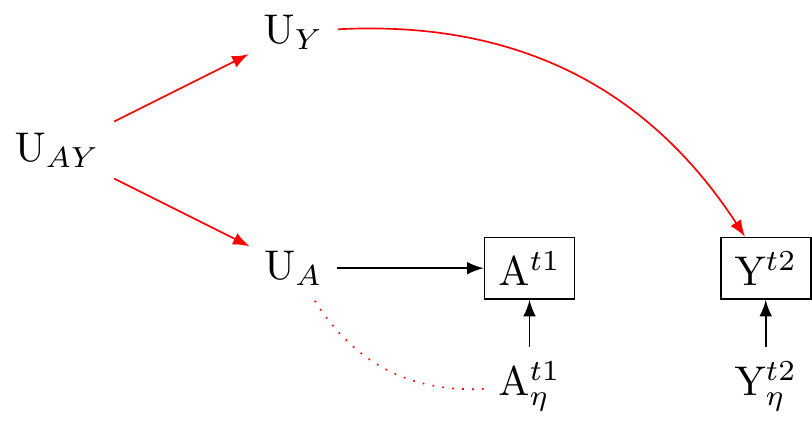
\includegraphics[width=0.8\textwidth,height=\textheight]{causal-dags_files/figure-pdf/fig-dag-dep-u-effect-1.pdf}

}

\caption{\label{fig-dag-dep-u-effect}Correlated undirected measurement
error can distort causal effect estimates under the null, indicated by
the red path.}

\end{figure}

\hypertarget{correlated-differential-directed-measurement-error}{%
\subsubsection{4. Correlated differential (directed) measurement
error}\label{correlated-differential-directed-measurement-error}}

Correlated differential (directed) measurement error occurs when the
measurement errors are related independently of the exposure, and the
exposure also affects levels of these correlated error terms. The
structure of this bias is presented in Figure~\ref{fig-dag-d-d}. Suppose
societies with stronger beliefs in Big Gods tend to record their
religious beliefs and social structures more meticulously than others.
Suppose further that religious elites conduct this record-keeping. The
errors may be both correlated and differential if societies with beliefs
in Big Gods tend to favour these religious elites, leading to biased
records.

Consider further the three-wave panel design, where we aim to estimate
the effect of self-reported religious service attendance on
self-reported monthly donations to charity. A set of confounders is
included at baseline, comprising previous measures of religious service
attendance and monthly donations to charity. Because our measures rely
on self-reports, they may be especially prone to measurement error.

Assume there is an unmeasured common cause affecting both the
measurement error of religious service attendance and the measurement
error of donations to charity. This bias might occur if individuals
consistently over- or under-report their religious service attendance
and donations due to social desirability bias.

In Part 3, we discussed how including the exposure measured at baseline
can reduce confounding in a three-wave panel design. By controlling for
the baseline exposure, we effectively adjust for any static
characteristics that cause a correlation between the exposure and
outcome.

Now for measurement error, including baseline measures could mitigate
the impact of these errors on causal effect estimation, provided the
errors are random and not systematically associated across time points.

To see this, let \(A_0\), \(A_1\) denote the exposure at baseline and
follow-up, and \(Y_0\), \(Y_1\) denote the outcome at baseline and
follow-up. The true values are denoted without primes, and the measured
values are with primes. We assume the measurement error is additive:

\(A'_0 = A_0 + UA_0\),

\(A'_1 = A_1 + UA_1\),

\(Y'_0 = Y_0 + UY_0\),

\(Y'_2 = Y_2 + UY_2\),

where \(UA_0\), \(UA_1\) are the measurement errors for the exposure at
baseline and follow-up, and \(UY_0\), \(UY_2\) are the measurement
errors for the outcome at baseline and follow-up. If the errors are
correlated, then \(Cov(UA_0, UY_0) \neq 0\) and/or
\(Cov(UA_1, UY_2) \neq 0\).

In a model that includes \(A'_0\) and \(Y'_0\) as covariates, the
estimated effect of \(A'_1\) on \(Y'_2\) identifies the effect of change
in the exposure from baseline to follow-up on the incidence effect.
Because our interest is in this incidence effect, we control for the
baseline exposure and outcome measures. This strategy will mitigate bias
arising from correlated errors if the following conditions hold:

\(E(UA_0) = E(UA_1)\) and \(E(UY_0) = E(UY_2)\) (i.e., the expectation
of the measurement errors does not change over time),

\(Cov(UA_0, UY_2) = Cov(UA_1, UY_2)\) (i.e., the correlation between the
errors does not change over time).

Thus, including baseline measurements in our model can mitigate
undirected measurement errors. However, this solution hinges on the
measurement error being undirected and non-differential concerning time.
If the measurement error varies over time or affects other variables in
the model, baseline measurement control will be inadequate for
confounding control (see: (\protect\hyperlink{ref-keogh2020}{Keogh
\emph{et al.} 2020})).

Consider a scenario where individuals who attend religious service more
at wave 1 acquire more substantial social desirability bias, becoming
more likely to over-report socially desirable behaviours or under-report
socially undesirable ones. The structure of this scenario is presented
in Figure~\ref{fig-dag-d-d}. If the measured outcome at wave 2 is
charitable giving, the increased social desirability bias could lead to
an overestimation of the actual level of giving. Suppose we compare
reported charity at wave 2 with reported religious attendance at wave 1.
If there is directed measurement bias we might falsely attribute the
apparent increase in charity to the increase in religious service
attendance, when, in reality, there was over-reporting from social
desirability bias that was induced by religious service attendance. Here
we can see that if the error of the outcome is affected by the exposure,
the causal effect of the increase in religious service on charitable
giving might be different from the association presented in the data.

Thus, although controlling for baseline exposure is a powerful strategy
for isolating incidence effects and controlling confounding, we have
seen that it is not a catch-all solution. Attention to the quality of
measures at all time points remains critical.

For instance, to avoid presentation bias, rather than asking whether one
has \emph{offered} help, we might ask participants in a multi-wave study
whether they have \emph{received help} -- under the assumption that if
the religious community is more altruistic than the secular community,
the probability of receiving help will be higher.

\begin{figure}

{\centering 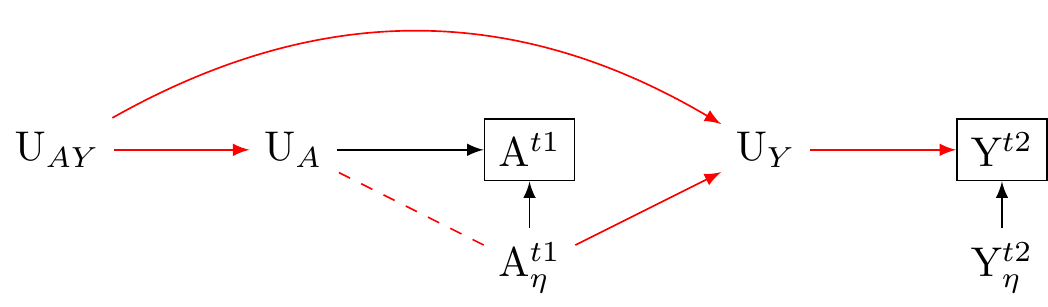
\includegraphics[width=1\textwidth,height=\textheight]{causal-dags_files/figure-pdf/fig-dag-d-d-1.pdf}

}

\caption{\label{fig-dag-d-d}Directed dependent (correlated) measurement
error leads to bias in causal effect estimates. Here, the exposure
affects the measurement error of the outcome. Additionally, the
measurement error of the exposure and outcome are correlated. These
dynamics open pathways for bias, indicated by the red paths. Sructural
sources of bias in measurement error must be evaluated, and sensitivity
analyses should be preformed to assess threats to causal inference.}

\end{figure}

\hypertarget{using-time-ordered-causal-diagrams-to-understand-threats-of-correlated-measurement-error-for-causal-inference-comparative-cultural-research}{%
\subsubsection{Using time-ordered causal diagrams to understand threats
of correlated measurement error for causal inference comparative
cultural
research}\label{using-time-ordered-causal-diagrams-to-understand-threats-of-correlated-measurement-error-for-causal-inference-comparative-cultural-research}}

To comprehend the structural features that might undermine causal
inferences in comparative cultural research, consider a simplified
scenario. Imagine that before conducting cultural comparisons, the
measurement errors of the exposure and outcome variables are
uncorrelated, as illustrated in Figure~\ref{fig-dag-uu-null}. While
measurement error can lead to a downward bias off the null, under the
null, no bias occurs.

However, when selecting study participants from different cultures --
cultures that inherently vary in interpretations and behaviours --- an
unmeasured bias under the null can occur, as shown in
Figure~\ref{fig-dag-dep-u-effect-selection}. To highlight this issue, we
modify the causal diagram in Figure~\ref{fig-dag-uu-null} to include
participant selection. This act of comparative selection creates a new
study population in which the error terms of measures become associated.
We cannot condition on cultural membership to block these associations,
as it was the act of conditioning that induced them in the new study
population.

If we did not undertake comparative sampling, the exposure and outcome
would be d-separated under the given scenario, yielding no bias for
separate studies, as shown in Figure~\ref{fig-dag-uu-null}. We cannot
resort to stratifying on culture to address this bias, as it is the act
of stratifying on culture that gives rise to correlated measurement
errors. Conducting separate analyses by culture precludes
generalisation, yet science seeks to find generalisations wherever it
can. Human scientists strive to identify functions supporting
transportable inferences wherever possible (see Part 2).

Yet, given the myriad ways the true structures of the world can align
with correlational models, we must be cautious when using conventional
invariance testing thresholds as the arbiters for cultural science. Such
tests should be considered exploratory tools. They can guide comparative
research, but must not replace careful scientific thinking, informed by
local expertise. In causal inference, decisions must be tailor-made to
fit the specific situation at hand.

\begin{figure}

{\centering \includegraphics[width=1\textwidth,height=\textheight]{causal-dags_files/figure-pdf/fig-dag-dep-u-effect-selection-1.pdf}

}

\caption{\label{fig-dag-dep-u-effect-selection}Measurement bias in
comparative cross-cultural research. Selection at baseline induces
correlations in the measurement error of the exposure and outcome.
Biasing paths are presented in red. Where selection induces error, we
might be better of conducting separate country-wide analyses.
Cross-cultural researchers should not assume that our interest in
generalisation, although scientifically desirable, can be supported from
the data we collect. Again, careful case-by-case assessments are
needed.}

\end{figure}

\hypertarget{using-time-ordered-causal-diagrams-to-understand-how-post-outcome-adjustment-may-diminish-threats-of-directed-measurement-error-in-cultural-evolutionary-research}{%
\subsubsection{Using time-ordered causal diagrams to understand how
post-outcome adjustment may diminish threats of directed measurement
error in cultural evolutionary
research}\label{using-time-ordered-causal-diagrams-to-understand-how-post-outcome-adjustment-may-diminish-threats-of-directed-measurement-error-in-cultural-evolutionary-research}}

Figure Figure~\ref{fig-dag-measure-selection-0} illustrates a situation
often encountered in the evolutionary science of historical cultures.
Let us assume that there is no relationship between the actual exposure,
\(A\), and actual outcome, \(Y\). Further, suppose that the outcome
influences the measurement error of the exposure, denoted as \(UA\).
This influence is assumed to be directional, opening a backdoor path
between the measured exposure, \(A^{\prime}\), and the measured outcome,
\(Y'\). (For simplicity, we will not consider that the outcome is
measured with error; this assumption does not alter the problem's
structure.) Scenarios akin to that shown in
Figure~\ref{fig-dag-measure-selection-0} frequently emerge in historical
evolutionary human science because history written by victors.

\begin{figure}

{\centering 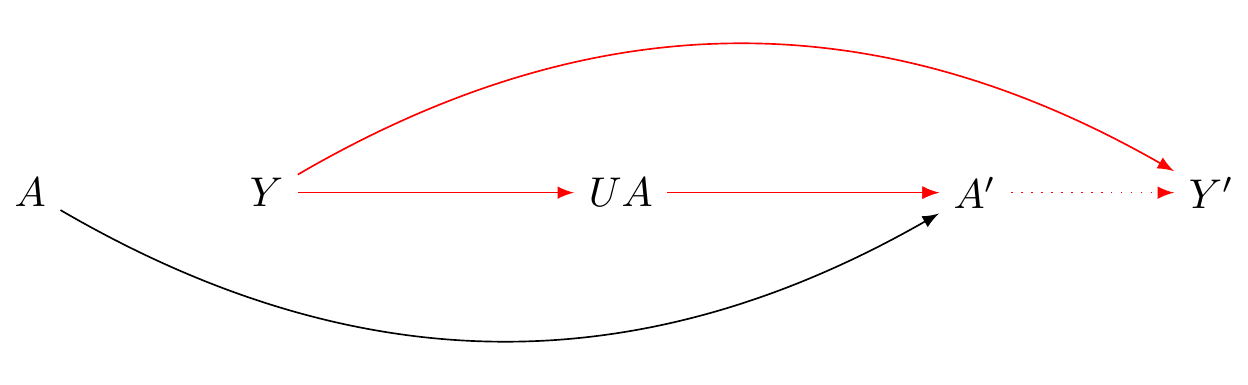
\includegraphics[width=1\textwidth,height=\textheight]{causal-dags_files/figure-pdf/fig-dag-measure-selection-0-1.pdf}

}

\caption{\label{fig-dag-measure-selection-0}The figure illustrates the
bias arising measurement error of A' caused by Y. Although A and Y are
independent, their measured counterparts, A' and Y', are not. The
systematic error introduced by changes in Y opens a biasing path,
signified in red.}

\end{figure}

Figure~\ref{fig-dag-measure-selection} exposes the structure of bias
where post-outcome adjustment is necessary to mitigate or eliminate
measurement bias instigated by the outcome itself. Assume our interest
lies in quantifying the influence of belief in Big gods on social
complexity. We assumed that highly complex societies amend history,
eliminating traces of beliefs in lesser gods. If traces of beliefs in
lesser gods were recoverable through sources such as language, cultural
evolutoinary researchers would obtain better effect estimates.
Figure~\ref{fig-dag-measure-selection} clarifies the intuition that
recovering ``echoes of the silenced'' is worthwhile for enhancing the
accuracy of our causal effect estimates.

\begin{figure}

{\centering 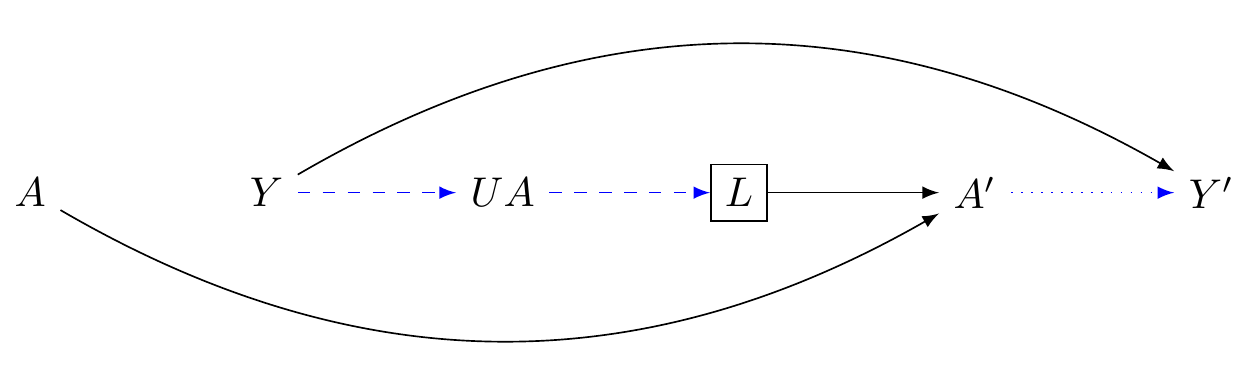
\includegraphics[width=1\textwidth,height=\textheight]{causal-dags_files/figure-pdf/fig-dag-measure-selection-1.pdf}

}

\caption{\label{fig-dag-measure-selection}Causal diagram elucidates how
refined measurements attenuate bias. By recovering measures undistorted
by past outcomes, we attenuate the directed measurement error. We
repesent this scenario on the graph by removing the path from Y to UA.}

\end{figure}

\hypertarget{using-time-ordered-causal-diagrams-to-clarify-the-structural-assumptions-of-latent-factor-models}{%
\subsubsection{Using time-ordered causal diagrams to clarify the
structural assumptions of latent factor
models}\label{using-time-ordered-causal-diagrams-to-clarify-the-structural-assumptions-of-latent-factor-models}}

Human evolutionary scientists who wish to collect time-series data by
measuring individuals over time in panel designs may consider using
multi-item constructs in their panel studies. What are the implications
of doing so? Multi-item constructs have long been favoured by
traditional psychometric theory. However, classical psychometric theory
developed without the benefit of causal approaches. VanderWeele argues
that difficulties surface when assessing the causal assumptions of
formative and reflective latent factor models
(\protect\hyperlink{ref-vanderweele2022}{VanderWeele 2022}). These
models are based on statistical formulations. However, the causal
inferences they embody cannot be determined solely by statistical
models. This discussion will concentrate on reflective models, although
the concerns raised are equally applicable to formative models, and I
refer interested readers to:
(\protect\hyperlink{ref-vanderweele2022}{VanderWeele 2022}).\footnote{In
  formative models, observed variables are perceived to generate the
  latent variable. This latent variable is assumed to be a composite of
  the observed variables, \(X_i\), mathematically expressed as
  \(\eta = \sum_i\lambda_i X_i\). The structural assumption is that a
  single latent variable causally influences the observed variables.
  This structural is depicted in
  Figure~\ref{fig-structural-assumptions-reflective-model}.}

\begin{figure}

{\centering 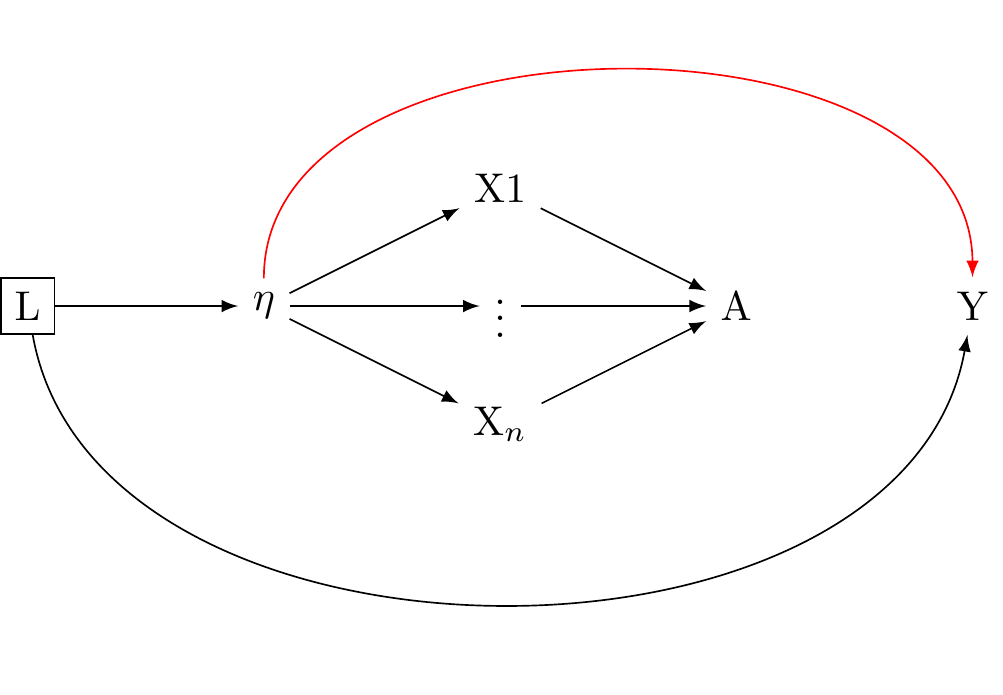
\includegraphics[width=0.8\textwidth,height=\textheight]{causal-dags_files/figure-pdf/fig-structural-assumptions-reflective-model-1.pdf}

}

\caption{\label{fig-structural-assumptions-reflective-model}Structural
assumptions of the reflective model imply a univariate reality causes
the outcome. These assumptions are strong because they exclude
multivariate causes of the indicators for constructs, as well as
independent effects of the indicators on outcomes. Blue line indicates
assumed causal path. The figure is adapted from VanderWeele: doi:
10.1097/EDE.0000000000001434}

\end{figure}

However, VanderWeele notes that the statistical model is consistent with
multiple causal models. The presumption that a univariate latent reality
underlies the reflective (and formative) latent factor models is a
stronger assumption than previously acknowledged. For example, an
alternative structural model equally compatible with the data is
presented in Figure~\ref{fig-dag_multivariate_reality_again}. Here,
multivariate reality gives rise to the indicators from which we draw our
measures. Indeed, for specific widely used measures, the assumption of a
univariate reality is so strong that they make testable assumptions.
VanderWeele and Vansteeland test the empirical examination assumptions
of widely used depression scales and find the assumptions fail
(\protect\hyperlink{ref-vanderweele2022b}{VanderWeele and Vansteelandt
2022}). Although we cannot generally determine which structural models
are accurate, the data rule out the univariate model in case that
VanderWeele and Vansteelandt
(\protect\hyperlink{ref-vanderweele2022b}{2022}) examine.

\begin{figure}

{\centering \includegraphics[width=0.6\textwidth,height=\textheight]{causal-dags_files/figure-pdf/fig-dag_multivariate_reality_again-1.pdf}

}

\caption{\label{fig-dag_multivariate_reality_again}Vanderweele's example
of an alternative structural model that is consistent with the
statistical model that underpins reflective construct models. Here, a
multivariate reality gives rise to the indicators from which we draw our
measures. Additional paths from the latent factors to the outcome are
presented in Blue. (Confounders are omited for simplicity). This figure
is adapted from VanderWeele: doi: 10.1097/EDE.0000000000001434}

\end{figure}

Although the assumptions of a univariate reality that underlie
traditional latent factor models are not generally credible, VanderWeele
suggests that construct measures can still find application in research.
On VanderWeele's view, the key to salvaging latent factor models is to
extend the theory of causal inference under multiple interventions to
latent factor models
(\protect\hyperlink{ref-vanderweele2022}{VanderWeele 2022}).
Specifically, by framing measured variables as functions of indicators
that may map onto a complex multivariate underlying reality, we may
approach them as coarsened indicators for that reality. As long as the
potential outcomes of these coarsened indicators are conditionally
independent of their treatment assignments and there is no unmeasured
confounding, we may assume the constructs to consistently estimate the
causal effects of the complex reality that gives rise to them.

While I agree with VanderWeele that the theory of causal inference under
multiple interventions might offer some redemption to factor models,
caution should still be exercised. Similar to the theory of causal
inference under multiple versions of treatments, there are situations
where guaranteeing conditional exchangeability might be unfeasible.
Furthermore, even when such assurance is possible, difficulties might
arise in interpreting the results or endorsing policy interventions. In
the following section, I develop another concern arising from threats to
confounding arising from directed measurement error in constructs.

\hypertarget{causal-diagrams-highlight-biases-arising-from-measurement-errors-within-constructs}{%
\subsubsection{Causal diagrams highlight biases arising from measurement
errors within
constructs}\label{causal-diagrams-highlight-biases-arising-from-measurement-errors-within-constructs}}

Consider a three-wave panel with the assumption that no unmeasured
confounding exists. We represent the exposure \(A\) as a function of
indicators, \(A_{f(A_1, A_2, ..., A_n)}\), representing a coarsened
state of a multivariate reality. Each component of this reality
corresponds to a structural element, represented as
\(\eta_{A_1}, \eta_{A_2}, ..., \eta_{A_n}\), each with associated error
terms, \(U\eta_{A_1}, U\eta_{A_2}, ..., U\eta_{A_n}\).

We can similarly conceptualise the outcome \(Y\), as a function of
indicators, \(Y_{f(Y_1, Y_2, ..., Y_n)}\), representing a latent
reality. This latent reality is composed of the components
\(\eta_{Y_1}, \eta_{Y_2}, ..., \eta_{Y_n}\), each with their
corresponding error terms
\(U\eta_{Y_1}, U\eta_{Y_2}, ..., U\eta_{Y_n}\). For simplicity, we leave
out baseline confounders and imagine a randomised experiment.

Figure~\ref{fig-dag-coarsen-measurement-error} depicts this assumed
reality and outlines potential confounding paths due to directed
measurement error from the indicators of the exposure, measured with
error, to the indicators or the outcome, measured with error. Each path
consists of a structural component \(\eta_{A_n}\) and its associated
error term \(U\eta_{Y_n}\). We identify three potential confounding
paths resulting from directed measurement error.

The potential for confounding from measurement error in panel designs
fundamentally relies on the relationships and dependencies among
variables, not their quantity. However, it is worth emphasising that, in
theory, an increase in the number of latent states or error terms may
enhance the potential for confounding. Under simplifying assumptions,
the potential direct paths from the exposure to the outcome are given by
the product of the number of components of the exposure and the number
of error terms associated with the outcome, symbolically represented as
\(\eta A_n \times U\eta_{Y_n}\). In this simplified scenario, each
latent variable connected to exposure could influence every error term
of an outcome, creating a complex network of confounding paths.

Causal diagrams, when applied to measurement error in latent factor
models, underscore the necessity of thorough scrutiny of construct
measures in evolutionary human sciences. Although no universal rule
exists, researchers may sometimes choose to use single-item measures.
Each case, however, necessitates a meticulous investigation of the
items' definitions, probable interpretations, and potential causal
implications over time. Composite scales can enhance efficiency. If
their underlying assumptions make sense, it is sensible to use them.
Yet, often these assumptions will not hold. Human evolutionary
scientists -- as well as other human scientists -- need to cultivate the
habits for evaluating the specifics of each research question within its
context.

\begin{figure}

{\centering 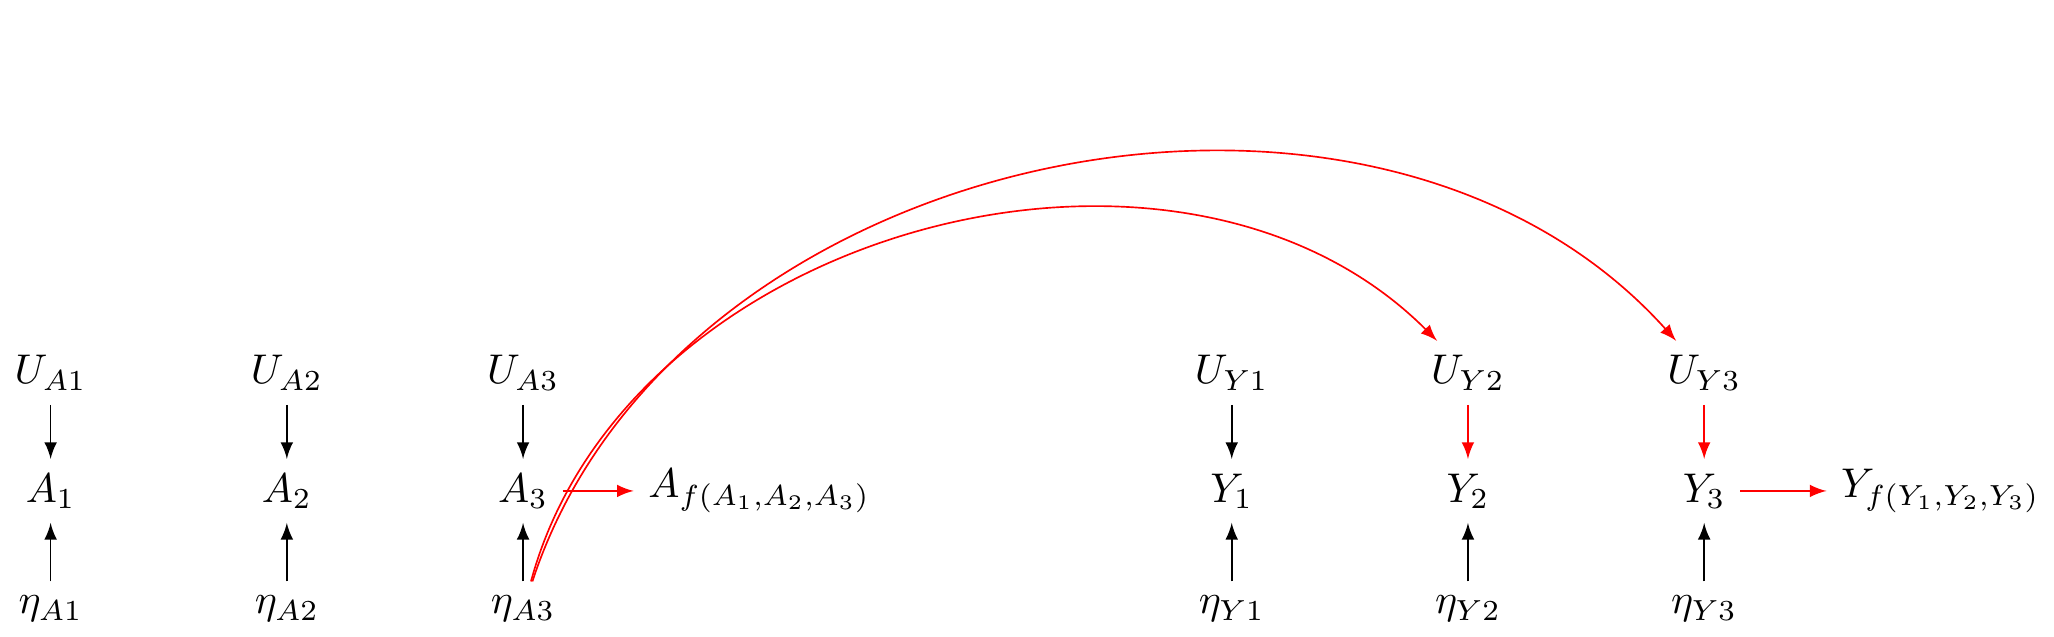
\includegraphics[width=1\textwidth,height=\textheight]{causal-dags_files/figure-pdf/fig-dag-coarsen-measurement-error-1.pdf}

}

\caption{\label{fig-dag-coarsen-measurement-error}Where there are many
indicators of a psychological construct, there are many opportunities
for additional confounding by directed measurement error.}

\end{figure}

\hypertarget{summary-part-5}{%
\subsubsection{Summary Part 5}\label{summary-part-5}}

Part 5 describes sources of bias from measurement error in repeated
measures data designs. We examined four types of measurement error bias,
assessing how each might skew inference. Although adjustments for the
baseline exposure and baseline outcome can reduce confounding -- and
isolate incidence effects -- the strategy is not a panacea. Often the
exposure, or the source of error in its measurement, may plausibly
affect the measurement of the outcome. In such cases, the correlations
we obtain may be biased indicators of causation.

Although there are methods for adjusting for measurement error that not
covered in this article, a host of useful resources exists, including
the works of Keogh \emph{et al.}
(\protect\hyperlink{ref-keogh2020}{2020}) Buonaccorsi
(\protect\hyperlink{ref-buonaccorsi2010}{2010}) Shi \emph{et al.}
(\protect\hyperlink{ref-shi2021}{2021}) Valeri \emph{et al.}
(\protect\hyperlink{ref-valeri2014}{2014}) and Bandalos
(\protect\hyperlink{ref-bandalos2018}{2018}). Additionally, sometimes
specialist knowledge will tell us about the direction of influence in
the error terms, whether positive or negative
(\protect\hyperlink{ref-suzuki2020}{Suzuki \emph{et al.} 2020};
\protect\hyperlink{ref-vanderweele2007a}{VanderWeele and Robins 2007a},
\protect\hyperlink{ref-vanderweele2010}{2010}). In these cases, we may
employ causal diagrams with signed paths to improve causal inferences
(\protect\hyperlink{ref-vanderweele2012}{VanderWeele and Hernán 2012}).
The purpose of this section has been to examine how causal diagrams can
be used to reveal sources of counfounding from measurement bias, how
measurement bias arises in settings of comparative cultural research,
why latent factor models claim too much, and why in some cases single
item measures might do better. Chronologically ordered causal diagrams,
once more, disclose imperatives not only for data analysis but also for
data collection. They underscore the need to devise and use measurement
tools that minimise error. Any they encourage us not to blindly adhere
to psychometric traditions but to instead contemplate causality in the
context of the question at hand.

\hypertarget{conclusions}{%
\subsection{Conclusions}\label{conclusions}}

Chronologically ordered causal diagrams provide significant enrichment
to causal inference endeavours. Their utility is not limited to just
modelling; they also serve as valuable guides for data collection. Used
judiciously and with a solid grasp of the assumptions required for
causal inference, causal diagrams can substantially enhance our pursuit
of accurate and robust causal understanding.

\hypertarget{summary-of-advice-tips}{%
\subsubsection{Summary of advice: Tips}\label{summary-of-advice-tips}}

\begin{enumerate}
\def\labelenumi{\arabic{enumi}.}
\item
  Clearly define all nodes on the graph. Ambiguity leads to confusion.
\item
  Simplify the graph. Keep only essential nodes and edges for clarifying
  the identification problem. Avoid clutter.
\item
  Define any novel conventions in your diagram explicitly. Do not assume
  familiarity.
\item
  Ensure acyclicity in the graph. This guarantees that a node cannot be
  its own ancestor, thereby eliminating circular paths.
\item
  Maintain chronological order spatially. Arrange nodes in temporal
  sequence, usually from left to right or top to bottom. Although it is
  not necessary to draw the sequence to scale, the order of events
  should be clear from the layout.
\item
  Time-stamp nodes. Causation happens over time; reflect this visually
  in the diagrams.
\item
  Be pragmatic. Employ a ``modified disjunctive cause criterion'' to
  reduce, if not eliminate, bias.
\item
  Draw nodes for unmeasured confounding where it aids confounding
  control strategies. Assume unmeasured confounding always exists,
  whether depicted on the graph or not. This necessitates sensitivity
  analyses of causal effect estimates.
\item
  Illustrate nodes for post-treatment selection. This facilitates
  understanding of potential sources of selection bias.
\item
  Apply a two-step strategy: Initially, isolate confounding bias and
  selection bias, then contemplate measurement bias using a secondary
  graph. This approach will foster clarity.\footnote{See Hernán and
    Robins (\protect\hyperlink{ref-hernuxe1n2023}{2023a}) p.125}
\end{enumerate}

\begin{enumerate}
\def\labelenumi{\arabic{enumi}.}
\setcounter{enumi}{10}
\item
  Expand graphs to clarify relevant bias structures if mediation or
  interaction is of interest. However, do not attempt to draw non-linear
  associations between variables.
\item
  Remember, causal diagrams are qualitative tools encoding assumptions
  about causal ancestries. They are compasses, not comprehensive
  atlases.
\end{enumerate}

\hypertarget{summary-of-advice-pitfalls}{%
\subsubsection{Summary of advice:
Pitfalls}\label{summary-of-advice-pitfalls}}

\begin{enumerate}
\def\labelenumi{\arabic{enumi}.}
\item
  Misunderstanding the role of causal diagrams within the framework of
  counter-factual data science.
\item
  The causal diagram contains variables without time indices. This
  omission may suggest that the researcher has not adequately considered
  the timing of events.
\item
  The graph has excessive nodes. No effort has been made to simplify the
  model by retaining only those nodes and edges essential for clarifying
  the identification problem.
\item
  The study is an experiment, but arrows are leading into the
  manipulation, revealing confusion.
\item
  Bias is incorrectly described. The exposure and outcome are
  d-separated, yet bias is claimed. This indicates a misunderstanding;
  the bias probably relates to generalisability or transportability, not
  to confounding.
\item
  Overlooking the representation of selection bias on the graph,
  particularly post-exposure selection bias from attrition or
  missingness.
\item
  Neglecting to use causal diagrams during the design phase of research
  before data collection.
\item
  Ignoring structural assumptions in classical measurement theory, such
  as in latent factor models, and blindly using factor measures.
\item
  Trying to represent interactions and non-linear dynamics on a causal
  diagram, which can lead to confusion about their purposes.
\item
  Failing to realise that structural equation models are not structural
  models. They are tools for statistical analysis, better termed as
  ``correlational equation models.'' Coefficients from these models
  often lack causal interpretations.
\item
  Neglecting the fact that conventional models such as multi-level (or
  mixed effects) models are unsuitable when treatment-confounder
  feedback is present. Illustrating treatment-confounder feedback on a
  graph underscores this point.\footnote{G-methods are appropriate for
    causal estimation in dynamic longitudinal settings. Their
    effectiveness notwithstanding, many evolutionary human scientists
    have not adopted them.{[}\^{}g-methods-cites{]} For good
    introductions see: Hernán and Robins
    (\protect\hyperlink{ref-hernuxe1n2023}{2023a}) Díaz \emph{et al.}
    (\protect\hyperlink{ref-duxedaz2021}{2021}) VanderWeele
    (\protect\hyperlink{ref-vanderweele2015}{2015}) Hoffman \emph{et
    al.} (\protect\hyperlink{ref-hoffman2022}{2022}) Hoffman \emph{et
    al.} (\protect\hyperlink{ref-hoffman2023}{2023}) Chatton \emph{et
    al.} (\protect\hyperlink{ref-chatton2020}{2020}) Shiba and Kawahara
    (\protect\hyperlink{ref-shiba2021}{2021}) Sjölander
    (\protect\hyperlink{ref-sjuxf6lander2016}{2016}) Breskin \emph{et
    al.} (\protect\hyperlink{ref-breskin2020}{2020}) VanderWeele
    (\protect\hyperlink{ref-vanderweele2009a}{2009b}) Vansteelandt
    \emph{et al.} (\protect\hyperlink{ref-vansteelandt2012}{2012}) Shi
    \emph{et al.} (\protect\hyperlink{ref-shi2021}{2021}).)}
\end{enumerate}

\begin{enumerate}
\def\labelenumi{\arabic{enumi}.}
\setcounter{enumi}{11}
\tightlist
\item
  Failing to recognise that simple models work for time series data with
  three measurement intervals. A repeated measures model is unnecessary
  for the three-wave design described in Part 3.
\end{enumerate}

\hypertarget{concluding-remarks}{%
\subsubsection{Concluding remarks}\label{concluding-remarks}}

Chronologically ordered causal diagrams show the necessity of
time-series data for answering quantitative causal questions. The demand
for time-series data collection in causal inference brings substantial
implications for research design, funding models, and the pace of
scientific discovery. Scientific progress will be contingent on our
institutional capacity to transition from a productivity model
reminiscent of an assembly line or counterfeit money press to a system
that nurtures long-term data collection.

\newpage{}

\hypertarget{references}{%
\subsection{References}\label{references}}

\hypertarget{refs}{}
\begin{CSLReferences}{1}{0}
\leavevmode\vadjust pre{\hypertarget{ref-bandalos2018}{}}%
Bandalos, DL (2018) \emph{Measurement theory and applications for the
social sciences}, Guilford Publications.

\leavevmode\vadjust pre{\hypertarget{ref-bareinboim2022}{}}%
Bareinboim, E, Tian, J, and Pearl, J (2022) Recovering from selection
bias in causal and statistical inference. In, 1st edn, Vol. 36, New
York, NY, USA: Association for Computing Machinery, 433450. Retrieved
from \url{https://doi.org/10.1145/3501714.3501740}

\leavevmode\vadjust pre{\hypertarget{ref-barrett2021}{}}%
Barrett, M (2021) \emph{Ggdag: Analyze and create elegant directed
acyclic graphs}. Retrieved from
\url{https://CRAN.R-project.org/package=ggdag}

\leavevmode\vadjust pre{\hypertarget{ref-basten2013}{}}%
Basten, C, and Betz, F (2013) Beyond work ethic: Religion, individual,
and political preferences. \emph{American Economic Journal: Economic
Policy}, \textbf{5}(3), 67--91.
doi:\href{https://doi.org/10.1257/pol.5.3.67}{10.1257/pol.5.3.67}.

\leavevmode\vadjust pre{\hypertarget{ref-becker2016}{}}%
Becker, SO, Pfaff, S, and Rubin, J (2016) Causes and consequences of the
protestant reformation. \emph{Explorations in Economic History},
\textbf{62}, 125.

\leavevmode\vadjust pre{\hypertarget{ref-breskin2020}{}}%
Breskin, A, Edmonds, A, Cole, SR, \ldots{} Adimora, AA (2020)
G-computation for policy-relevant effects of interventions on
time-to-event outcomes. \emph{International Journal of Epidemiology},
\textbf{49}(6), 2021--2029.
doi:\href{https://doi.org/10.1093/ije/dyaa156}{10.1093/ije/dyaa156}.

\leavevmode\vadjust pre{\hypertarget{ref-bulbulia2022}{}}%
Bulbulia, JA (2022) A workflow for causal inference in cross-cultural
psychology. \emph{Religion, Brain \& Behavior}, \textbf{0}(0), 1--16.
doi:\href{https://doi.org/10.1080/2153599X.2022.2070245}{10.1080/2153599X.2022.2070245}.

\leavevmode\vadjust pre{\hypertarget{ref-bulbulia2021}{}}%
Bulbulia, J, Schjoedt, U, Shaver, JH, Sosis, R, and Wildman, WJ (2021)
Causal inference in regression: Advice to authors. \emph{Religion, Brain
\& Behavior}, \textbf{11}(4), 353360.

\leavevmode\vadjust pre{\hypertarget{ref-buonaccorsi2010}{}}%
Buonaccorsi, JP (2010) \emph{Measurement error: Models, methods, and
applications}, New York: Chapman; Hall/CRC.
doi:\href{https://doi.org/10.1201/9781420066586}{10.1201/9781420066586}.

\leavevmode\vadjust pre{\hypertarget{ref-chatton2020}{}}%
Chatton, A, Le Borgne, F, Leyrat, C, \ldots{} Foucher, Y (2020)
G-computation, propensity score-based methods, and targeted maximum
likelihood estimator for causal inference with different covariates
sets: a comparative simulation study. \emph{Scientific Reports},
\textbf{10}(1), 9219.
doi:\href{https://doi.org/10.1038/s41598-020-65917-x}{10.1038/s41598-020-65917-x}.

\leavevmode\vadjust pre{\hypertarget{ref-cinelli2022}{}}%
Cinelli, C, Forney, A, and Pearl, J (2022) A Crash Course in Good and
Bad Controls. \emph{Sociological Methods \& Research},
00491241221099552.
doi:\href{https://doi.org/10.1177/00491241221099552}{10.1177/00491241221099552}.

\leavevmode\vadjust pre{\hypertarget{ref-cole2008}{}}%
Cole, SR, and Hernán, MA (2008) Constructing inverse probability weights
for marginal structural models. \emph{American Journal of Epidemiology},
\textbf{168}(6), 656--664.
doi:\href{https://doi.org/10.1093/aje/kwn164}{10.1093/aje/kwn164}.

\leavevmode\vadjust pre{\hypertarget{ref-cole2010}{}}%
Cole, SR, Platt, RW, Schisterman, EF, \ldots{} Poole, C (2010)
Illustrating bias due to conditioning on a collider. \emph{International
Journal of Epidemiology}, \textbf{39}(2), 417--420.
doi:\href{https://doi.org/10.1093/ije/dyp334}{10.1093/ije/dyp334}.

\leavevmode\vadjust pre{\hypertarget{ref-collinson2007}{}}%
Collinson, P (2007) \emph{The reformation: A history}, Vol. 19, Modern
Library.

\leavevmode\vadjust pre{\hypertarget{ref-decoulanges1903}{}}%
De Coulanges, F (1903) \emph{La cité antique: Étude sur le culte, le
droit, les institutions de la grèce et de rome}, Hachette.

\leavevmode\vadjust pre{\hypertarget{ref-deffner2022}{}}%
Deffner, D, Rohrer, JM, and McElreath, R (2022) A Causal Framework for
Cross-Cultural Generalizability. \emph{Advances in Methods and Practices
in Psychological Science}, \textbf{5}(3), 25152459221106366.
doi:\href{https://doi.org/10.1177/25152459221106366}{10.1177/25152459221106366}.

\leavevmode\vadjust pre{\hypertarget{ref-duxedaz2021}{}}%
Díaz, I, Williams, N, Hoffman, KL, and Schenck, EJ (2021) Non-parametric
causal effects based on longitudinal modified treatment policies.
\emph{Journal of the American Statistical Association}.
doi:\href{https://doi.org/10.1080/01621459.2021.1955691}{10.1080/01621459.2021.1955691}.

\leavevmode\vadjust pre{\hypertarget{ref-edwards2015}{}}%
Edwards, JK, Cole, SR, and Westreich, D (2015) All your data are always
missing: Incorporating bias due to measurement error into the potential
outcomes framework. \emph{International Journal of Epidemiology},
\textbf{44}(4), 14521459.

\leavevmode\vadjust pre{\hypertarget{ref-gawthrop1984}{}}%
Gawthrop, R, and Strauss, G (1984) Protestantism and literacy in early
modern germany. \emph{Past \& Present}, (104), 3155.

\leavevmode\vadjust pre{\hypertarget{ref-greenland1977}{}}%
Greenland, S (1977) Response and follow-up bias in cohort studies.
\emph{American Journal of Epidemiology}, \textbf{106}(3), 184--187.
doi:\href{https://doi.org/10.1093/oxfordjournals.aje.a112451}{10.1093/oxfordjournals.aje.a112451}.

\leavevmode\vadjust pre{\hypertarget{ref-greenland1999}{}}%
Greenland, S, Pearl, J, and Robins, JM (1999) Causal diagrams for
epidemiologic research. \emph{Epidemiology (Cambridge, Mass.)},
\textbf{10}(1), 37--48.

\leavevmode\vadjust pre{\hypertarget{ref-hernuxe1n2017}{}}%
Hernán, MA (2017) Invited commentary: Selection bias without colliders
\textbar{} american journal of epidemiology \textbar{} oxford academic.
\emph{American Journal of Epidemiology}, \textbf{185}(11), 10481050.
Retrieved from \url{https://doi.org/10.1093/aje/kwx077}

\leavevmode\vadjust pre{\hypertarget{ref-hernuxe1n2008}{}}%
Hernán, MA, Alonso, A, Logan, R, \ldots{} Robins, JM (2008)
Observational studies analyzed like randomized experiments: An
application to postmenopausal hormone therapy and coronary heart
disease. \emph{Epidemiology}, \textbf{19}(6), 766.
doi:\href{https://doi.org/10.1097/EDE.0b013e3181875e61}{10.1097/EDE.0b013e3181875e61}.

\leavevmode\vadjust pre{\hypertarget{ref-hernuxe1n2009}{}}%
Hernán, MA, and Cole, SR (2009) Invited commentary: Causal diagrams and
measurement bias. \emph{American Journal of Epidemiology},
\textbf{170}(8), 959--962.
doi:\href{https://doi.org/10.1093/aje/kwp293}{10.1093/aje/kwp293}.

\leavevmode\vadjust pre{\hypertarget{ref-hernuxe1n2004}{}}%
Hernán, MA, Hernández-Díaz, S, and Robins, JM (2004) A structural
approach to selection bias. \emph{Epidemiology}, \textbf{15}(5),
615--625. Retrieved from \url{https://www.jstor.org/stable/20485961}

\leavevmode\vadjust pre{\hypertarget{ref-hernuxe1n2006}{}}%
Hernán, MA, and Robins, JM (2006) Estimating causal effects from
epidemiological data. \emph{Journal of Epidemiology \& Community
Health}, \textbf{60}(7), 578586.

\leavevmode\vadjust pre{\hypertarget{ref-hernuxe1n2023a}{}}%
Hernán, MA, and Robins, JM (2023b) \emph{Causal inference: What if?},
Taylor \& Francis. Retrieved from
\url{https://books.google.co.nz/books?id=/_KnHIAAACAAJ}

\leavevmode\vadjust pre{\hypertarget{ref-hernuxe1n2023}{}}%
Hernán, MA, and Robins, JM (2023a) \emph{Causal inference: What if?},
Taylor \& Francis. Retrieved from
\url{https://books.google.co.nz/books?id=/_KnHIAAACAAJ}

\leavevmode\vadjust pre{\hypertarget{ref-hernuxe1n2016}{}}%
Hernán, MA, Sauer, BC, Hernández-Díaz, S, Platt, R, and Shrier, I
(2016a) Specifying a target trial prevents immortal time bias and other
self-inflicted injuries in observational analyses. \emph{Journal of
Clinical Epidemiology}, \textbf{79}, 7075.

\leavevmode\vadjust pre{\hypertarget{ref-hernuxe1n2016a}{}}%
Hernán, MA, Sauer, BC, Hernández-Díaz, S, Platt, R, and Shrier, I
(2016b) Specifying a target trial prevents immortal time bias and other
self-inflicted injuries in observational analyses. \emph{Journal of
Clinical Epidemiology}, \textbf{79}, 7075.

\leavevmode\vadjust pre{\hypertarget{ref-hernuxe1n2022}{}}%
Hernán, MA, Wang, W, and Leaf, DE (2022b) Target trial emulation: A
framework for causal inference from observational data. \emph{JAMA},
\textbf{328}(24), 2446--2447.
doi:\href{https://doi.org/10.1001/jama.2022.21383}{10.1001/jama.2022.21383}.

\leavevmode\vadjust pre{\hypertarget{ref-hernuxe1n2022a}{}}%
Hernán, MA, Wang, W, and Leaf, DE (2022a) Target trial emulation: A
framework for causal inference from observational data. \emph{JAMA},
\textbf{328}(24), 2446--2447.
doi:\href{https://doi.org/10.1001/jama.2022.21383}{10.1001/jama.2022.21383}.

\leavevmode\vadjust pre{\hypertarget{ref-hoffman2023}{}}%
Hoffman, KL, Salazar-Barreto, D, Rudolph, KE, and Díaz, I (2023)
Introducing longitudinal modified treatment policies: A unified
framework for studying complex exposures.
doi:\href{https://doi.org/10.48550/arXiv.2304.09460}{10.48550/arXiv.2304.09460}.

\leavevmode\vadjust pre{\hypertarget{ref-hoffman2022}{}}%
Hoffman, KL, Schenck, EJ, Satlin, MJ, \ldots{} Díaz, I (2022) Comparison
of a target trial emulation framework vs cox regression to estimate the
association of corticosteroids with COVID-19 mortality. \emph{JAMA
Network Open}, \textbf{5}(10), e2234425.
doi:\href{https://doi.org/10.1001/jamanetworkopen.2022.34425}{10.1001/jamanetworkopen.2022.34425}.

\leavevmode\vadjust pre{\hypertarget{ref-holland1986}{}}%
Holland, PW (1986) Statistics and causal inference. \emph{Journal of the
American Statistical Association}, \textbf{81}(396), 945960.

\leavevmode\vadjust pre{\hypertarget{ref-hume1902}{}}%
Hume, D (1902) \emph{Enquiries Concerning the Human Understanding: And
Concerning the Principles of Morals}, Clarendon Press.

\leavevmode\vadjust pre{\hypertarget{ref-keogh2020}{}}%
Keogh, RH, Shaw, PA, Gustafson, P, \ldots{} Freedman, LS (2020) STRATOS
guidance document on measurement error and misclassification of
variables in observational epidemiology: Part 1{\textemdash}Basic theory
and simple methods of adjustment. \emph{Statistics in Medicine},
\textbf{39}(16), 2197--2231.
doi:\href{https://doi.org/10.1002/sim.8532}{10.1002/sim.8532}.

\leavevmode\vadjust pre{\hypertarget{ref-lauritzen1990}{}}%
Lauritzen, SL, Dawid, AP, Larsen, BN, and Leimer, H-G (1990)
Independence properties of directed markov fields. \emph{Networks},
\textbf{20}(5), 491505.

\leavevmode\vadjust pre{\hypertarget{ref-lewis1973}{}}%
Lewis, D (1973) Causation. \emph{The Journal of Philosophy},
\textbf{70}(17), 556--567.
doi:\href{https://doi.org/10.2307/2025310}{10.2307/2025310}.

\leavevmode\vadjust pre{\hypertarget{ref-leyrat2019}{}}%
Leyrat, C, Seaman, SR, White, IR, \ldots{} Williamson, EJ (2019)
Propensity score analysis with partially observed covariates: How should
multiple imputation be used? \emph{Statistical Methods in Medical
Research}, \textbf{28}(1), 319.

\leavevmode\vadjust pre{\hypertarget{ref-lu2022}{}}%
Lu, H, Cole, SR, Howe, CJ, and Westreich, D (2022) Toward a Clearer
Definition of Selection Bias When Estimating Causal Effects.
\emph{Epidemiology (Cambridge, Mass.)}, \textbf{33}(5), 699--706.
doi:\href{https://doi.org/10.1097/EDE.0000000000001516}{10.1097/EDE.0000000000001516}.

\leavevmode\vadjust pre{\hypertarget{ref-mathur2018}{}}%
Mathur, MB, Ding, P, Riddell, CA, and VanderWeele, TJ (2018) Website and
r package for computing e-values. \emph{Epidemiology (Cambridge,
Mass.)}, \textbf{29}(5), e45.

\leavevmode\vadjust pre{\hypertarget{ref-mcelreath2020}{}}%
McElreath, R (2020) \emph{Statistical rethinking: A bayesian course with
examples in r and stan}, CRC press.

\leavevmode\vadjust pre{\hypertarget{ref-murray2021}{}}%
Murray, EJ, Marshall, BDL, and Buchanan, AL (2021a) Emulating target
trials to improve causal inference from agent-based models.
\emph{American Journal of Epidemiology}, \textbf{190}(8), 1652--1658.
doi:\href{https://doi.org/10.1093/aje/kwab040}{10.1093/aje/kwab040}.

\leavevmode\vadjust pre{\hypertarget{ref-murray2021a}{}}%
Murray, EJ, Marshall, BDL, and Buchanan, AL (2021b) Emulating target
trials to improve causal inference from agent-based models.
\emph{American Journal of Epidemiology}, \textbf{190}(8), 1652--1658.
doi:\href{https://doi.org/10.1093/aje/kwab040}{10.1093/aje/kwab040}.

\leavevmode\vadjust pre{\hypertarget{ref-naimi2017}{}}%
Naimi, AI, Cole, SR, and Kennedy, EH (2017) An introduction to g
methods. \emph{International Journal of Epidemiology}, \textbf{46}(2),
756--762.
doi:\href{https://doi.org/10.1093/ije/dyw323}{10.1093/ije/dyw323}.

\leavevmode\vadjust pre{\hypertarget{ref-nalle1987}{}}%
Nalle, ST (1987) Inquisitors, priests, and the people during the
catholic reformation in spain. \emph{The Sixteenth Century Journal},
557587.

\leavevmode\vadjust pre{\hypertarget{ref-ogburn2022}{}}%
Ogburn, EL, Sofrygin, O, Díaz, I, and Laan, MJ van der (2022) Causal
inference for social network data. \emph{Journal of the American
Statistical Association}, \textbf{0}(0), 1--15.
doi:\href{https://doi.org/10.1080/01621459.2022.2131557}{10.1080/01621459.2022.2131557}.

\leavevmode\vadjust pre{\hypertarget{ref-pearl1988}{}}%
Pearl, J (1988) \emph{Probabilistic reasoning in intelligent systems:
Networks of plausible inference}, Morgan kaufmann.

\leavevmode\vadjust pre{\hypertarget{ref-pearl1995}{}}%
Pearl, J (1995) Causal diagrams for empirical research.
\emph{Biometrika}, \textbf{82}(4), 669--688.
doi:\href{https://doi.org/10.1093/biomet/82.4.669}{10.1093/biomet/82.4.669}.

\leavevmode\vadjust pre{\hypertarget{ref-pearl2009}{}}%
Pearl, J (2009a) \emph{\href{https://doi.org/10.1214/09-SS057}{Causal
inference in statistics: An overview}}.

\leavevmode\vadjust pre{\hypertarget{ref-pearl2009a}{}}%
Pearl, J (2009b) \emph{Causality}, Cambridge University Press.

\leavevmode\vadjust pre{\hypertarget{ref-pearl2022}{}}%
Pearl, J, and Bareinboim, E (2022) External validity: From do-calculus
to transportability across populations. In, 1st edn, Vol. 36, New York,
NY, USA: Association for Computing Machinery, 451482. Retrieved from
\url{https://doi.org/10.1145/3501714.3501741}

\leavevmode\vadjust pre{\hypertarget{ref-pearl2018}{}}%
Pearl, J, and Mackenzie, D (2018) \emph{The book of why: The new science
of cause and effect}, Basic books.

\leavevmode\vadjust pre{\hypertarget{ref-pearl1995a}{}}%
Pearl, J, and Robins, JM (1995) Probabilistic evaluation of sequential
plans from causal models with hidden variables. In, Vol. 95, Citeseer,
444453.

\leavevmode\vadjust pre{\hypertarget{ref-pishgar2021}{}}%
Pishgar, F, Greifer, N, Leyrat, C, and Stuart, E (2021) MatchThem::
Matching and weighting after multiple imputation. \emph{The R Journal},
\textbf{13}(2), 292305.
doi:\href{https://doi.org/10.32614/RJ-2021-073}{10.32614/RJ-2021-073}.

\leavevmode\vadjust pre{\hypertarget{ref-richardson2013}{}}%
Richardson, TS, and Robins, JM (2013) Single world intervention graphs
(SWIGs): A unification of the counterfactual and graphical approaches to
causality. \emph{Center for the Statistics and the Social Sciences,
University of Washington Series. Working Paper}, \textbf{128}(30), 2013.

\leavevmode\vadjust pre{\hypertarget{ref-robins1986}{}}%
Robins, J (1986) A new approach to causal inference in mortality studies
with a sustained exposure period{\textemdash}application to control of
the healthy worker survivor effect. \emph{Mathematical Modelling},
\textbf{7}(9), 1393--1512.
doi:\href{https://doi.org/10.1016/0270-0255(86)90088-6}{10.1016/0270-0255(86)90088-6}.

\leavevmode\vadjust pre{\hypertarget{ref-robins1999}{}}%
Robins, JM, Greenland, S, and Hu, F-C (1999) Estimation of the causal
effect of a time-varying exposure on the marginal mean of a repeated
binary outcome. \emph{Journal of the American Statistical Association},
\textbf{94}(447), 687--700.
doi:\href{https://doi.org/10.1080/01621459.1999.10474168}{10.1080/01621459.1999.10474168}.

\leavevmode\vadjust pre{\hypertarget{ref-rohrer2018}{}}%
Rohrer, JM (2018) Thinking clearly about correlations and causation:
Graphical causal models for observational data. \emph{Advances in
Methods and Practices in Psychological Science}, \textbf{1}(1), 2742.

\leavevmode\vadjust pre{\hypertarget{ref-rubin1976}{}}%
Rubin, DB (1976) Inference and missing data. \emph{Biometrika},
\textbf{63}(3), 581--592.
doi:\href{https://doi.org/10.1093/biomet/63.3.581}{10.1093/biomet/63.3.581}.

\leavevmode\vadjust pre{\hypertarget{ref-rubin2005}{}}%
Rubin, DB (2005) Causal inference using potential outcomes: Design,
modeling, decisions. \emph{Journal of the American Statistical
Association}, \textbf{100}(469), 322--331. Retrieved from
\url{https://www.jstor.org/stable/27590541}

\leavevmode\vadjust pre{\hypertarget{ref-shi2021}{}}%
Shi, B, Choirat, C, Coull, BA, VanderWeele, TJ, and Valeri, L (2021)
CMAverse: A suite of functions for reproducible causal mediation
analyses. \emph{Epidemiology}, \textbf{32}(5), e20e22.

\leavevmode\vadjust pre{\hypertarget{ref-shiba2021}{}}%
Shiba, K, and Kawahara, T (2021) Using propensity scores for causal
inference: Pitfalls and tips. \emph{Journal of Epidemiology},
\textbf{31}(8), 457463.

\leavevmode\vadjust pre{\hypertarget{ref-sjuxf6lander2016}{}}%
Sjölander, A (2016) Regression standardization with the R package
stdReg. \emph{European Journal of Epidemiology}, \textbf{31}(6),
563--574.
doi:\href{https://doi.org/10.1007/s10654-016-0157-3}{10.1007/s10654-016-0157-3}.

\leavevmode\vadjust pre{\hypertarget{ref-stuart2015}{}}%
Stuart, EA, Bradshaw, CP, and Leaf, PJ (2015) Assessing the
Generalizability of Randomized Trial Results to Target Populations.
\emph{Prevention Science}, \textbf{16}(3), 475--485.
doi:\href{https://doi.org/10.1007/s11121-014-0513-z}{10.1007/s11121-014-0513-z}.

\leavevmode\vadjust pre{\hypertarget{ref-suzuki2016}{}}%
Suzuki, E, Mitsuhashi, T, Tsuda, T, and Yamamoto, E (2016) A typology of
four notions of confounding in epidemiology. \emph{Journal of
Epidemiology}, \textbf{27}(2), 49--55.
doi:\href{https://doi.org/10.1016/j.je.2016.09.003}{10.1016/j.je.2016.09.003}.

\leavevmode\vadjust pre{\hypertarget{ref-suzuki2020}{}}%
Suzuki, E, Shinozaki, T, and Yamamoto, E (2020) Causal Diagrams:
Pitfalls and Tips. \emph{Journal of Epidemiology}, \textbf{30}(4),
153--162.
doi:\href{https://doi.org/10.2188/jea.JE20190192}{10.2188/jea.JE20190192}.

\leavevmode\vadjust pre{\hypertarget{ref-suzuki2014}{}}%
Suzuki, E, and Yamamoto, E (2014) Further refinements to the
organizational schema for causal effects. \emph{Epidemiology},
\textbf{25}(4), 618.
doi:\href{https://doi.org/10.1097/EDE.0000000000000114}{10.1097/EDE.0000000000000114}.

\leavevmode\vadjust pre{\hypertarget{ref-swanson1967}{}}%
Swanson, GE (1967) Religion and regime: A sociological account of the
reformation.

\leavevmode\vadjust pre{\hypertarget{ref-swanson1971}{}}%
Swanson, GE (1971) Interpreting the reformation. \emph{The Journal of
Interdisciplinary History}, \textbf{1}(3), 419446. Retrieved from
\url{http://www.jstor.org/stable/202620}

\leavevmode\vadjust pre{\hypertarget{ref-tripepi2007}{}}%
Tripepi, G, Jager, KJ, Dekker, FW, Wanner, C, and Zoccali, C (2007)
Measures of effect: Relative risks, odds ratios, risk difference, and
{`}number needed to treat{'}. \emph{Kidney International},
\textbf{72}(7), 789--791.
doi:\href{https://doi.org/10.1038/sj.ki.5002432}{10.1038/sj.ki.5002432}.

\leavevmode\vadjust pre{\hypertarget{ref-valeri2014}{}}%
Valeri, L, Lin, X, and VanderWeele, TJ (2014) Mediation analysis when a
continuous mediator is measured with error and the outcome follows a
generalized linear model. \emph{Statistics in Medicine},
\textbf{33}(28), 48754890.

\leavevmode\vadjust pre{\hypertarget{ref-vantongeren2020}{}}%
Van Tongeren, DR, DeWall, CN, Chen, Z, Sibley, CG, and Bulbulia, J
(2020) Religious residue: Cross-cultural evidence that religious
psychology and behavior persist following deidentification.
\emph{Journal of Personality and Social Psychology}.

\leavevmode\vadjust pre{\hypertarget{ref-vanderweele2015}{}}%
VanderWeele, T (2015) \emph{Explanation in causal inference: Methods for
mediation and interaction}, Oxford University Press.

\leavevmode\vadjust pre{\hypertarget{ref-vanderweele2009}{}}%
VanderWeele, TJ (2009a) Concerning the consistency assumption in causal
inference. \emph{Epidemiology}, \textbf{20}(6), 880.
doi:\href{https://doi.org/10.1097/EDE.0b013e3181bd5638}{10.1097/EDE.0b013e3181bd5638}.

\leavevmode\vadjust pre{\hypertarget{ref-vanderweele2009a}{}}%
VanderWeele, TJ (2009b) Marginal structural models for the estimation of
direct and indirect effects. \emph{Epidemiology}, 1826.

\leavevmode\vadjust pre{\hypertarget{ref-vanderweele2018}{}}%
VanderWeele, TJ (2018) On well-defined hypothetical interventions in the
potential outcomes framework. \emph{Epidemiology}, \textbf{29}(4), e24.
doi:\href{https://doi.org/10.1097/EDE.0000000000000823}{10.1097/EDE.0000000000000823}.

\leavevmode\vadjust pre{\hypertarget{ref-vanderweele2019}{}}%
VanderWeele, TJ (2019) Principles of confounder selection.
\emph{European Journal of Epidemiology}, \textbf{34}(3), 211--219.
doi:\href{https://doi.org/10.1007/s10654-019-00494-6}{10.1007/s10654-019-00494-6}.

\leavevmode\vadjust pre{\hypertarget{ref-vanderweele2022}{}}%
VanderWeele, TJ (2022) Constructed measures and causal inference:
Towards a new model of measurement for psychosocial constructs.
\emph{Epidemiology}, \textbf{33}(1), 141.
doi:\href{https://doi.org/10.1097/EDE.0000000000001434}{10.1097/EDE.0000000000001434}.

\leavevmode\vadjust pre{\hypertarget{ref-vanderweele2013}{}}%
VanderWeele, TJ, and Hernan, MA (2013) Causal inference under multiple
versions of treatment. \emph{Journal of Causal Inference},
\textbf{1}(1), 120.

\leavevmode\vadjust pre{\hypertarget{ref-vanderweele2012}{}}%
VanderWeele, TJ, and Hernán, MA (2012) Results on differential and
dependent measurement error of the exposure and the outcome using signed
directed acyclic graphs. \emph{American Journal of Epidemiology},
\textbf{175}(12), 1303--1310.
doi:\href{https://doi.org/10.1093/aje/kwr458}{10.1093/aje/kwr458}.

\leavevmode\vadjust pre{\hypertarget{ref-vanderweele2014}{}}%
VanderWeele, TJ, and Knol, MJ (2014) A tutorial on interaction.
\emph{Epidemiologic Methods}, \textbf{3}(1), 3372.

\leavevmode\vadjust pre{\hypertarget{ref-vanderweele2020}{}}%
VanderWeele, TJ, Mathur, MB, and Chen, Y (2020) Outcome-wide
longitudinal designs for causal inference: A new template for empirical
studies. \emph{Statistical Science}, \textbf{35}(3), 437466.

\leavevmode\vadjust pre{\hypertarget{ref-vanderweele2007a}{}}%
VanderWeele, TJ, and Robins, JM (2007a) Directed acyclic graphs,
sufficient causes, and the properties of conditioning on a common
effect. \emph{American Journal of Epidemiology}, \textbf{166}(9),
1096--1104.
doi:\href{https://doi.org/10.1093/aje/kwm179}{10.1093/aje/kwm179}.

\leavevmode\vadjust pre{\hypertarget{ref-vanderweele2007}{}}%
VanderWeele, TJ, and Robins, JM (2007b) Four types of effect
modification: a classification based on directed acyclic graphs.
\emph{Epidemiology (Cambridge, Mass.)}, \textbf{18}(5), 561--568.
doi:\href{https://doi.org/10.1097/EDE.0b013e318127181b}{10.1097/EDE.0b013e318127181b}.

\leavevmode\vadjust pre{\hypertarget{ref-vanderweele2010}{}}%
VanderWeele, TJ, and Robins, JM (2010) Signed directed acyclic graphs
for causal inference. \emph{Journal of the Royal Statistical Society
Series B: Statistical Methodology}, \textbf{72}(1), 111--127.
doi:\href{https://doi.org/10.1111/j.1467-9868.2009.00728.x}{10.1111/j.1467-9868.2009.00728.x}.

\leavevmode\vadjust pre{\hypertarget{ref-vanderweele2022b}{}}%
VanderWeele, TJ, and Vansteelandt, S (2022) A statistical test to reject
the structural interpretation of a latent factor model. \emph{Journal of
the Royal Statistical Society Series B: Statistical Methodology},
\textbf{84}(5), 20322054.

\leavevmode\vadjust pre{\hypertarget{ref-vansteelandt2012}{}}%
Vansteelandt, S, Bekaert, M, and Lange, T (2012) Imputation strategies
for the estimation of natural direct and indirect effects.
\emph{Epidemiologic Methods}, \textbf{1}(1), 131158.

\leavevmode\vadjust pre{\hypertarget{ref-watts2016}{}}%
Watts, J, Bulbulia, J. A., Gray, RD, and Atkinson, QD (2016) Clarity and
causality needed in claims about big gods., \textbf{39}, 4142.
doi:\href{https://doi.org/d4qp}{d4qp}.

\leavevmode\vadjust pre{\hypertarget{ref-watts2018}{}}%
Watts, J, Sheehan, O, Bulbulia, Joseph A, Gray, RD, and Atkinson, QD
(2018) Christianity spread faster in small, politically structured
societies. \emph{Nature Human Behaviour}, \textbf{2}(8), 559564.
doi:\href{https://doi.org/gdvnjn}{gdvnjn}.

\leavevmode\vadjust pre{\hypertarget{ref-weber1905}{}}%
Weber, M (1905) \emph{The protestant ethic and the spirit of capitalism:
And other writings}, Penguin.

\leavevmode\vadjust pre{\hypertarget{ref-weber1993}{}}%
Weber, M (1993) \emph{The sociology of religion}, Beacon Press.

\leavevmode\vadjust pre{\hypertarget{ref-westreich2010}{}}%
Westreich, D, and Cole, SR (2010) Invited commentary: positivity in
practice. \emph{American Journal of Epidemiology}, \textbf{171}(6).
doi:\href{https://doi.org/10.1093/aje/kwp436}{10.1093/aje/kwp436}.

\leavevmode\vadjust pre{\hypertarget{ref-westreich2015}{}}%
Westreich, D, Edwards, JK, Cole, SR, Platt, RW, Mumford, SL, and
Schisterman, EF (2015) Imputation approaches for potential outcomes in
causal inference. \emph{International Journal of Epidemiology},
\textbf{44}(5), 17311737.

\leavevmode\vadjust pre{\hypertarget{ref-wheatley1971}{}}%
Wheatley, P (1971) \emph{The pivot of the four quarters : A preliminary
enquiry into the origins and character of the ancient chinese city},
Edinburgh University Press. Retrieved from
\url{https://cir.nii.ac.jp/crid/1130000795717727104}

\leavevmode\vadjust pre{\hypertarget{ref-williams2021}{}}%
Williams, NT, and Díaz, I (2021) \emph{Lmtp: Non-parametric causal
effects of feasible interventions based on modified treatment policies}.
doi:\href{https://doi.org/10.5281/zenodo.3874931}{10.5281/zenodo.3874931}.

\leavevmode\vadjust pre{\hypertarget{ref-wright1920}{}}%
Wright, S (1920) The relative importance of heredity and environment in
determining the piebald pattern of guinea-pigs. \emph{Proceedings of the
National Academy of Sciences of the United States of America},
\textbf{6}(6), 320.

\leavevmode\vadjust pre{\hypertarget{ref-wright1923}{}}%
Wright, S (1923) The theory of path coefficients a reply to niles's
criticism. \emph{Genetics}, \textbf{8}(3), 239.

\leavevmode\vadjust pre{\hypertarget{ref-zhang2023}{}}%
Zhang, J, Dashti, SG, Carlin, JB, Lee, KJ, and Moreno-Betancur, M (2023)
Should multiple imputation be stratified by exposure group when
estimating causal effects via outcome regression in observational
studies? \emph{BMC Medical Research Methodology}, \textbf{23}(1), 42.
doi:\href{https://doi.org/10.1186/s12874-023-01843-6}{10.1186/s12874-023-01843-6}.

\end{CSLReferences}

\newpage{}

\hypertarget{appendix-1-review-of-vanderweeles-theory-of-causal-inference-under-multiple-versions-of-treatment}{%
\subsection{Appendix 1: Review of VanderWeele's theory of causal
inference under multiple versions of
treatment}\label{appendix-1-review-of-vanderweeles-theory-of-causal-inference-under-multiple-versions-of-treatment}}

We denote an average causal effect as the change in the expected
potential outcomes when all units receive one level of treatment
compared to another.

Let \(\delta\) denote the causal estimand on the difference scale
\((\mathbb{E}[Y^1 - Y^0])\). The causal effect identification can be
expressed as:

\[ \delta = \sum_l \left( \mathbb{E}[Y|A=a,l] - \mathbb{E}[Y|A=a^*,l] \right) P(l)\]

The theory of causal inference with multiple treatment versions provides
a conceptual framework for causal inference in observational studies.
Suppose we can assume that for each treatment version, the outcome under
that version equals the observed outcome when that version is
administered, conditional on baseline covariates and satisfaction of
other assumptions. In that case, we can consistently estimate causal
contrasts, even when treatments vary.

This approach interprets treatment indicator \(A\) as multiple actual
treatment versions \(K\). Furthermore, if we can assume conditional
independence, meaning there is no confounding for the effect of \(K\) on
\(Y\) given \(L\), we have: \(Y(k)\coprod A|K,L\).

This condition implies that, given \(L\), \(A\) adds no additional
information about \(Y\) after accounting for \(K\) and \(L\). If
\(Y = Y(k)\) for \(K = k\) and \(Y(k)\) is independent of \(K\),
conditional on \(L\), we can interpret \(A\) as a simplified indicator
of \(K\) (\protect\hyperlink{ref-vanderweele2013}{VanderWeele and Hernan
2013}). This scenario is depicted in
Figure~\ref{fig-dag_multiple_version_treatment_dag}.

With the necessary assumptions in place, we can derive consistent causal
effects. The causal effect can be expressed

\[\delta = \sum_{k,l} \left( \mathbb{E}[Y(k)|l] P(k|a,l) P(l) - \mathbb{E}[Y(k)|l] P(k|a^*,l) P(l) \right) \]

This setup is akin to a randomised trial where individuals, stratified
by covariate \(L\), are assigned a treatment version \(K\). This
assignment comes from the distribution of \(K\) for the
\((A = 1, L = l)\) subset. The control group receives a randomly
assigned \(K\) version from the \((A = 0, L = l)\) distribution.

\begin{figure}

{\centering \includegraphics[width=1\textwidth,height=\textheight]{causal-dags_files/figure-pdf/fig-dag_multiple_version_treatment_dag-1.pdf}

}

\caption{\label{fig-dag_multiple_version_treatment_dag}Causal inference
under multiple versions of treatment. Here, (A) may be regarded as a
coarseneed indicator of (K)}

\end{figure}

The theory of causal inference under multiple versions of treatment
reveal that consistent causal effect estimates are possible even when
treatments exhibit variability
(\protect\hyperlink{ref-vanderweele2013}{VanderWeele and Hernan 2013}).
In Part 5, I explored VanderWeele's application of this theory to latent
factor models, where the presumption of a single underlying reality for
the items that constitute constructs can be challenged
(\protect\hyperlink{ref-vanderweele2022}{VanderWeele 2022}).
Furthermore, I described additional complications not addressed by this
theory extension arising from measurement error. Specifically, the
possibility that directed or correlated error terms for the exposure and
outcome could undermine inference.



\end{document}
